\documentclass[10pt,a4paper]{book}
\usepackage{gensymb}
\usepackage{graphicx}
\usepackage{caption}
\usepackage{subcaption}
\usepackage[version=4]{mhchem}
\usepackage{hyperref}
\usepackage{pdflscape}
\usepackage{multirow}
\usepackage{array}
%-------------------------------------------------------------------------------
\begin{document}
%-------------------------------------------------------------------------------
\begin{titlepage}
\title{Glazes--for the Self-reliant Potter}
\date{1993}
\author{Henrik Norsker, James Danisch}
\maketitle
\end{titlepage}
%-------------------------------------------------------------------------------
\tableofcontents
%-------------------------------------------------------------------------------
\chapter*{Acknowledgements}
The original book is entitled \textit{Glazes--for the Self-Reliant Potter}, 
published in 1993.

DOI: 10.1007/978-3-663-06865-5

ISBN: 9783663068655 (online) 9783528020675 (print)

This document was compiled by Erik Haugsby from the source material provided 
via the CD3WD:
%-------------------------------------------------------------------------------
\begin{verbatim}
http://www.fastonline.org/CD3WD_40/CD3WD/APPRTECH/G17GLE/EN/B483.HTM
\end{verbatim}
%-------------------------------------------------------------------------------
I have made all attempts to preserve the original text and formating. The 
possibility of minor or unavoidable changes in layout and formatting, as well 
as unintentional errors in transcribing the original text, cannot be excluded.

Should you find any errors or omissions, I would greatly appreciate you either 
notifying me \href{mailto:e@erikhaugsby.com}{by email}, or initiating a pull 
request via Git.
%-------------------------------------------------------------------------------
\section*{The authors:}
%-------------------------------------------------------------------------------
\subsection*{Henrik Norsker} 
Henrik Norsker has been making pottery since 1970. He left his 
pottery workshop in Denmark in 1976 to establish a pottery school in a village 
in Tanzania. Since then he has continued working in developing countries with 
promotion of small scale ceramics industries. Besides Tanzania he has been 
employed in ceramics projects in Burma, Bangladesh and Nepal.
%-------------------------------------------------------------------------------
\subsection*{James Danisch} 
James Danisch has been making, selling and experimenting with 
ceramics since 1963. He has taught college level ceramics in Scotland and 
California, and has conducted workshops in the US, South America and Canada. 
From 1984 to 1992, he has been working with small scale and rural ceramics 
development in Nepal. His articles on ceramics have been published in several 
magazines, and he has studied traditional and he has studied traditional and 
modern techniques in Europe, Nepal, India, Thailand, Burma, South America and 
Mexico.
%-------------------------------------------------------------------------------
\subsection*{The Deutsches Zentrum f\"{u}r Entwicklungstechnologien}
Deutsches Zentrum f\"{u}r Entwicklungstechnologien-GATE

Deutsches Zentrum f\"{u}r Entwicklungstechnologien--GATE--stands for German 
Appropriate Technology Exchange. It was founded in 1978 as a special division 
of the Deutsche Gesellschaft f\"{u}r Technische Zusammenarbeit (GTZ) GmbH. GATE 
is a 
centre for the dissemination and promotion of appropriate technologies for 
developing countries. GATE defines ``Appropriate technologies'' as those which 
are suitable and acceptable in the light of economic, social and cultural 
criteria. They should contribute to socio-economic development whilst ensuring 
optimal utilization of resources and minimal detriment to the environment. 
Depending on the case at hand a traditional, intermediate or highly-developed 
can be the ``appropriate'' one. GATE focusses its work on the key areas:
%-------------------------------------------------------------------------------
\begin{itemize}
\item Dissemination of Appropriate Technologies: 

Collecting, processing and disseminating information on technologies 
appropriate to the needs of the developing countries: ascertaining the 
technological requirements of Third World countries: support in the form of 
personnel, material and equipment to promote the development and adaptation of 
technologies for developing countries.

\item Environmental Protection:

The growing importance of ecology and environmental protection require better 
coordination and harmonization of projects. In order to tackle these tasks more 
effectively, a coordination center was set up within GATE in 1985.
\end{itemize}
%-------------------------------------------------------------------------------
GATE has entered into cooperation agreements with a number of technology 
centres in Third World countries.

GATE offers a free information service on appropriate technologies for all 
public and private development institutions in developing countries, dealing 
with the development, adaptation, introduction and application of technologies.

Deutsche Gesellschaft f\"{u}r Technische Zusammenarbeit (GTZ) GmbH

The government-owned GTZ operates in the field of Technical Cooperation. 2200 
German experts are working together with partners from about 100 countries of 
Africa, Asia and Latin America in projects covering practically every sector of 
agriculture, forestry, economic development, social services and institutional 
and material infrastructure. The GTZ is commissioned to do this work both by 
the Government of the Federal Republic of Germany and by other government or 
semi-government authorities.

The GTZ activities encompass:
%-------------------------------------------------------------------------------
\begin{itemize}
\item appraisal, technical planning, control and supervision of technical 
cooperation projects commissioned by the Government of the Federal Republic or 
by other authorities

\item providing an advisory service to other agencies also working on 
development projects

\item the recruitment, selection, briefing, assignment, administration of 
expert personnel and their welfare and technical backstopping during their 
period of assignment

\item provision of materials and equipment for projects, planning work, 
selection, purchasing and shipment to the developing countries

\item management of all financial obligations to the partner-country.
\end{itemize}
%-------------------------------------------------------------------------------
Deutsches Zentrum f\"{u}r Entwicklungstechnologien--GATE:

Deutsche Gesellschaft f\"{u}r Technische Zusammenarbeit (GTZ) GmbH

P.O. Box 5180

D-65726 Eschborn

Federal Republic of Germany


Tel.: (06196) 79-0

Telex: 41523-0 gtz d

Fax: (06196) 797352


\chapter{Introduction and Scope}
There are already many books in the world on the subject of ceramic glazes. So 
the obvious question is: why yet another book on the subject? The authors have 
worked together for several years in a ceramics development project in Nepal, 
which is based on using local raw materials and resources. There are few 
existing books which offer much help in this area, especially working in the 
low temperature range from 900\degree C--1100\degree C, where lead glazes 
have been the tradition but which now, with greater understanding of health 
hazards, need to be replaced with lead-free glazes. This book is intended to 
provide practical information for ceramists working in developing countries, 
with little access to the prepared and controlled glaze materials available in 
industrialized nations.

Glazes are at one and the same time the area of most fascination and most 
difficulty for potters. Most potters have little inclination or time to devote 
to developing glazes, faced as they are by the daily need to produce for the 
market. However, there often are times when familiar glazes suddenly stop 
working correctly or special glazes are required for customers. This book 
offers guidelines for developing and altering glazes, understanding where 
problems with glazes come from, and standard procedures for testing and 
developing glazes when there is no laboratory equipment available. It has been 
written for potters who have little knowledge of chemistry and mathematics.
%-------------------------------------------------------------------------------
\section{Glaze-Making: Using Local Materials As Far As Possible}
Most small producers of glazed ceramics will use glazes that are prepared by a 
company specializing in supplying industry. However, these glazes are often 
unreliable, as big companies tend to serve large-scale producers and have 
little interest in the special glazes needed by small industries. For that 
reason, the small producer is often forced to rely on his own glaze production, 
with little or no laboratory equipment available. Additionally, the small 
producer does not usually have access to raw materials at reasonable prices, so 
he must use locally available raw materials that do not have an accurate 
chemical analysis.
%-------------------------------------------------------------------------------
\section{Glaze and Clay Systems}
The producer must think carefully before starting production. When a particular 
glaze is wanted, it must work with the available clay body, production system 
and firing system. 

For example, if you only have low-temperature red clay available, your glazes 
must work at around 1050\degree C. If you only have coal available for firing, 
you must make sure that it will work for your product. The following chapters 
provide information which will help you to make these decisions.
%-------------------------------------------------------------------------------
\chapter{The Nature of Glazes}
%-------------------------------------------------------------------------------
\section{Glass and Glaze, the Benefit of Glaze}
Glass is a useful material that has been known for thousands of years. It can 
be produced in many different shapes for many purposes, and it has many useful 
qualities: it is transparent, hard, resistant to chemicals, and can have many 
colors.

Glaze is a special type of glass, made for coating ceramic products. Whereas 
glass is suitable for forming into bottles or windows, glaze is different 
because it is applied on a ceramic surface and must form a hard, durable 
coating after being melted in the kiln. It must not run off the product and 
must stay on the product after firing without cracking.
%-------------------------------------------------------------------------------
\section{Glaze-Making is Difficult}
Because glaze before firing looks nothing like the finished product and because 
we are not able to directly understand what happens when glaze melts at high 
temperatures, making glazes is very difficult. We must try to understand which 
materials melt at certain temperatures and what happens when materials are 
combined. It requires a lot of direct experience before you start to understand 
causes and effects. In this way it is like cooking: we are familiar with 
cooking because we know the raw materials, and by trial and error we have a 
good idea of what the finished meal will be like. However, imagine that you are 
in a foreign country with unfamiliar food in the market and you want to make a 
meal: How do you start? The best way is with a cookbook full of recipes and a 
local friend to tell you if the result is correct or not. This book is intended 
as a cookbook for the independent potter.

Although by just reading this book and experimenting with it you will probably 
be able to make glazes after some time, there is no substitute for learning 
about glazes from an experienced teacher, who can save you a lot of time by 
guiding you in proven directions.
%-------------------------------------------------------------------------------
\section{History of Glazes}
Unglazed ceramics have been in existence for over 10,000 years. It has only 
been in the last 2000 years that there have been glazed ceramics and only in 
the last 100 years that a scientific approach to glaze making was developed. 
For that reason, glazes still occupy a mysterious area somewhere between 
science and magic.

The first glazes were probably invented in middle eastern countries, where 
there naturally exist deposits of sodium and potassium compounds (soda ash and 
pearl ash) that melt at low temperatures (800\degree --1000\degree C). By 
chance, early potters discovered that some clays when put in the fire developed 
a shiny surface. These self-glazing clays are known as ``Egyptian paste''. They 
are not very useful for making household items, being difficult to form.
The next step was to develop these substances so that they could be applied to 
the surface of pottery clay in order to give it the desirable qualities of a 
hard, shiny, easy-to-clean and durable surface. Because early potters did not 
have the technology to reach high firing temperatures, they had to use 
materials with low melting points, mainly sodium, potassium and lead compounds. 

Glaze development had to be done by trial and error, since these early potters 
had no idea of chemistry. This took a lot of time and effort, and naturally 
successful glazes were closely guarded secrets. These early glazes were often 
soft and not durable, and had problems such as cracking and eventually falling 
off the pot. Additionally, glazes based on lead were poisonous both for the 
potters who worked with them and for users.

It was only when potters learned to reach high temperatures that truly 
permanent ceramics were developed. There are many more common chemicals and 
minerals that melt above 1100\degree C to form glazes, and clay that is fired 
to these high temperatures is also much stronger and resistant to water.
%-------------------------------------------------------------------------------
\section{Glaze Classification}
Although there are many different ways to classify glazes, the simplest way to 
understand them is according to the firing temperature. The useful range of 
temperatures for glaze melting is from 900\degree --1300\degree C. In this 
book, we talk about two different categories of glaze:
%-------------------------------------------------------------------------------
\begin{itemize}
\item low temperature from 900-1100\degree C, called earthenware
\item high temperature from 1100-1300\degree C, called stoneware
\end{itemize} 
%-------------------------------------------------------------------------------
These two categories are used because they require different raw materials as 
the main ingredients of the glaze.
%------------------------------------------------------------------------------
\chapter{Temperature Ranges and Requirements}
%-------------------------------------------------------------------------------
\section{What is Temperature?}
Temperature means the amount of heat energy in a material. We raise the 
temperature of a material by providing it with heat energy, using a fire or 
electricity. What effect does this have on a material? We know that many 
familiar substances can exist in different states of solid, liquid and gas. For 
example, water can exist as ice, liquid water or steam. What is different about 
it? Only the temperature. All materials consist of atoms and molecules which 
are in constant motion. The amount of motion depends on the temperature. Cold 
materials have less motion and therefore appear solid to us (e.g. ice). When 
the temperature is increased, the motion of the molecules becomes greater and 
they can move more freely around each other (e.g. water). When the temperature 
is increased even more, the molecules become very active, as we can see when 
water boils. Then the molecules are even less bonded together and we see gas 
(e.g. steam).

Similarly, glazes are solid when they are cold (at room temperature), liquid 
when they are heated sufficiently (in the kiln), and become gas when they are 
heated too much.

It is also important to understand the relationship between clay and glaze. 
Most common red clay (such as brick clay) melts by 1100\degree C. This makes it 
useful for forming low temperature products. 1200\degree C, it can be used as a 
glaze.
%-------------------------------------------------------------------------------
\section{Low-Temperature Range (900--1000\degree C)}
Products called earthenware, whiteware, low-temperature ceramics, and terra 
cotta are all fired in the range of 900--1100\degree C. We will call these 
products 
generally "earthenware". What they have in common are clay bodies that develop 
their maximum strength in this range, and glazes that are based on low-melting 
compounds such as lead, sodium and potassium.
%-------------------------------------------------------------------------------
\subsection{Advantages and Disadvantages}
%-------------------------------------------------------------------------------
\subsubsection{Advantages}
Low temperature ceramics have the advantage of easy firing--it is much simpler 
to construct kilns and burner systems that have to reach no more than 
1100\degree C, and fuel costs are lower. Bright colors are possible in this 
range. Most common clays cannot be fired higher than this.
%-------------------------------------------------------------------------------
\subsubsection{Disadvantages}
Earthenware is often not as strong as high temperature ware, because the clay 
does not become vitreous. This means that it also has some porosity (the 
property of absorbing water) with the result that earthenware products often do 
not hold water unless the glaze is perfectly fitted to the body. Also, it is 
easier to chip the glaze away from the clay.

Historically, many earthenware glazes were based on poisonous lead because it 
is easy to melt: nowadays this is not a problem because lead can be replaced by 
non-poisonous materials.

Modern earthenware glazes are usually based on frits, which are expensive--the 
lower firing cost must be compared to the higher cost of the glaze.
%-------------------------------------------------------------------------------
\subsection{Clay and Glaze Characteristics}
%-------------------------------------------------------------------------------
\subsubsection{Earthenware Clay}
Common red-burning clay is normally used, often mixed with talcum powder to 
increase its firing range. In many countries, red clay which contains lime is 
used because it makes it easier to formulate glazes that do not craze (crack). 
White firing clay bodies are often based on talc, ball clay and fluxes to make 
them harder.
%-------------------------------------------------------------------------------
\subsubsection{Earthenware Glaze}
Earthenware glazes are based on low-melting materials, mainly lead oxide (white 
lead oxide, red lead oxide), sodium and boron compounds (soda ash, borax, boric 
acid) and potassium compounds (pearl ash, also known as potassium carbonate). 
Usually it is necessary to use these compounds in the form of frits (see 
chapter on frits).
%-------------------------------------------------------------------------------
\subsection{Raw Material Requirements}
Most of the raw materials for low temperature glazes can be obtained from 
commonly available sources. They include: local clays, wood and rice husk ash, 
limestone, and even soap powder (based on sodium and boron compounds). 
Materials such as borax must be obtained from chemical suppliers. Ready-made 
frits can be obtained from glaze suppliers, but in many locations it is 
necessary to make them from raw materials.
%-------------------------------------------------------------------------------
\section{High-Temperature Range (1100--1300\degree C)}
Types of ware fired in this range are known as stoneware and porcelain.
%-------------------------------------------------------------------------------
\subsection{Advantages and Disadvantages}
%-------------------------------------------------------------------------------
\subsubsection{Advantages}
High temperature products are generally stronger, more  acid and 
abrasion-resistant. Raw materials do not require fritting. The clay is more 
vitreous and thus does not have problems of water seepage.
%-------------------------------------------------------------------------------
\subsubsection{Disadvantages}
Kilns for high temperatures require more sophisticated bricks and kiln 
furniture, and better burner systems. Fuel costs are higher.
%-------------------------------------------------------------------------------
\subsection{Appropriate Products}
High temperature products include stoneware utilitarian items, whiteware of 
various types, porcelain and electrical insulators.
%-------------------------------------------------------------------------------
\subsection{Clay and Glaze Characteristics}
%-------------------------------------------------------------------------------
\subsubsection{Stoneware Clay}
Clay body raw materials are limited to those clays which can withstand high 
temperatures without melting: fireclays, ball clays, china clays, "stoneware" 
clays. Most bodies also include feldspar to cause vitrification, which prevents 
water seepage through the body.
%-------------------------------------------------------------------------------
\subsubsection{Stoneware Glaze}
High temperature glaze is easier to make than the low temperature sort, mainly 
because it is not necessary to frit the ingredients.
%-------------------------------------------------------------------------------
\subsection{Raw Material Requirements}
Most stoneware and porcelain glazes are based on feldspar, quartz, limestone 
and clay, with other ingredients to provide specific properties of surface, 
color etc.
%-------------------------------------------------------------------------------
\section{Firing Systems and Glaze Effects}
Different types of kilns and fuels have specific effects on glaze color and 
surface.
%-------------------------------------------------------------------------------
\subsection{Oil, Gas, Wood, Coal, Electricity, Other}
These are the main options for fuel. Each fuel requires a different kiln design 
and burner system. You must first decide which fuel is most available and most 
economical. The choice of fuel will determine whether products can be 
open-fired on shelves, or whether it is necessary to use saggers to protect the 
glaze from ash and contamination from dirty fuel.

The cost of fuel should be thought about very carefully. One kg of fuel 
produces a certain amount of heat. Heat is usually measured in calories or in 
British Thermal Units (BTU). One calorie is the amount of heat required to 
raise the temperature of one cubic centimeter of water 1\degree C. The table at 
page 170 shows the heat value of different fuels. Because a calorie is very 
small, the usual unit of heat is expressed as kilocalories (kilo = 1000, so 1 
kilocalorie = 1000 calories).

A particular kiln, loaded with an average number of products and fired to a 
specific temperature, will usually require the same amount of fuel each time, 
since it requires a specific number of calories to convert raw clay and glaze 
into finished ceramics. When you know the total kg of products and the total 
cost of one firing, it is easy to calculate the cost per kg of product:

\(Total~Cost/Total~KG = Cost~per~KG\)

You can also calculate the total number of calories required to do one firing. 
If you are using kerosene, you can find from the table that one lifer of 
kerosene supplies about 12,000 kilocalories of heat. So, if you use 80 liters 
to do a firing, the calculation is:

\(Total~fuel*(kilocalories~per~unit) = total~kilocalories~required\)

\(80*12,000=960,000~kilocalories\)

When deciding on the type of fuel to use, you should find out the cost per 
kilocalorie for different fuels in your area.
%------------------------------------------------------------------------------
\subsubsection{Oil}
Oil is available in many different forms, all of which can be used by the 
potter, including kerosene, diesel, furnace oil, and waste crankcase oil. 
Kerosene is the most clean-burning (without too much smoke or impurities), and 
waste crankcase oil is the dirtiest to use. Normally, products can be 
open-fired, but oil will produce some discoloration. For high quality 
whiteware, saggars may be necessary. Oil is suitable for high or low 
temperatures.

Oil provides between 9000 and 11000 kilocalories per kg.
%------------------------------------------------------------------------------
\subsubsection{Gas}
Gas is available as natural gas, producer gas or liquid propane gas. Where gas 
is available at a reasonable cost (compared to other fuels), it is the easiest 
fuel to use. Gas is very clean-burning, does not require saggars, and the 
burners are also simple to manufacture locally. It is suitable for any 
temperature.
%------------------------------------------------------------------------------
\subsubsection{Wood}
Almost any kind of wood can be used for firing kilns. Nowadays, wood is a 
scarce resource in most countries and more and more it is being replaced by 
other fuels. Firing with wood is labor-intensive. Because it produces a large 
volume of ash, it is usually necessary to fire the ware in saggers. It is 
suitable for any temperature.

On the other hand, wood is a renewable resource and in many areas of the world 
it is produced as a cash crop, which makes it appropriate to use.

The calorific value of wood is difficult to calculate, because it depends on 
the type of wood, whether it is wet or dry, and the efficiency of burning. Dry 
wood can supply between 3000 and 4500 kilocalories per kg, whereas the same 
wood when wet may produce only half the calories.
%------------------------------------------------------------------------------
\subsubsection{Coal}
Coal comes in many different grades, all of which are suitable for firing 
kilns. Firing with coal is labor-intensive, but in many countries it is the 
cheapest fuel available. Coal also produces ash and impurities, so it is 
usually necessary to fire the ware in saggars. It is best for high 
temperatures, but can be used at any temperature.

Coal can provide between 4500 and 7700 kilocalories per kg.
%------------------------------------------------------------------------------
\subsubsection{Electricity}
Electric kilns are practical for the small producer where there is a reliable 
source of electricity. Because there is no combustion, electricity is the 
cleanest fuel of all. Electric kilns fire very evenly and do not require 
saggers. Electricity is best for temperatures up to 1100\degree C.
%------------------------------------------------------------------------------
\subsubsection{Other Fuels}
These include tires, which burn very well but produce a lot of smoke, and also 
produce poisonous gases. They can be used in kilns designed to burn wood or 
coal. Some brick industries use scrap asphalt from roads as fuel. Also in this 
category are such fuels as brushwood, sawdust and rice husk. Most of these are 
dirty-burning, so require the use of saggers. They are best for low 
temperatures.
%------------------------------------------------------------------------------
\subsection{Oxidation and Reduction}
To understand oxidation and reduction, it is necessary to know how fuel burns. 
All fuel produces heat when it combines with the oxygen in the air. As anyone 
knows who has made a wood fire, if there is plenty of air the fire burns hot 
and clean, with little smoke. This is called an oxidation fire. If the air is 
reduced, there will be less heat and more smoke. This is called a reduction (or 
reducing) fire, which simply means reducing the amount of oxygen. So:
%------------------------------------------------------------------------------
\begin{itemize}
\item Oxidation firing means there is plenty of air and no smoke.
\item Reduction firing means there is little air and more smoke.
\end{itemize}
%------------------------------------------------------------------------------
Glazes will have different colors and surfaces depending on whether they are 
fired in oxidation or reduction conditions. Oxidation has its greatest effect 
on the metallic oxides that are used to create color in glazes. 

For example:
%------------------------------------------------------------------------------
\begin{center}
        \renewcommand{\arraystretch}{1.5}
        \begin{tabular}{|c|c|c|}\hline
\textbf{Oxide}&\textbf{Oxidation}&\textbf{Reduction}\\\hline\hline
%------------------------------------------------------------------------------
Red Iron Oxide&Brown&Red-Brown, Black\\\hline
%------------------------------------------------------------------------------
Copper Oxide&Green, Blue&Red\\\hline
%------------------------------------------------------------------------------
\end{tabular}
\end{center}
%------------------------------------------------------------------------------
Iron also changes from a grey color to a red color when it rusts. This is 
because oxide from the air-combines with the metal and forms iron oxide.

In firing, it is difficult to exactly control the amount of oxidation or 
reduction. Many beautiful glazes can be obtained in reduction firing, so it is 
widely used for decorative stoneware, and for lusterware. However, the results 
are variable and difficult to reproduce every time, and even in one kiln-load 
there will be differences. For that reason, most producers who need to supply a 
uniform product use oxidation firing.
%------------------------------------------------------------------------------
\subsection{Vapor Glazing}
In vapor glazing techniques, the glaze is not applied to the product before 
firing in the usual manner. Instead, glaze is introduced into the kiln through 
the firebox at the end of the firing, when there is enough heat to change the 
glaze into vapor form. The most common material for vapor glazing is ordinary 
salt. At temperatures above 1100\degree C, salt breaks down into sodium and 
chlorine vapor, which circulates through the kiln. The sodium is attracted to 
silica in the clay and forms a strong, durable glaze. Salt glazing is used 
mainly for sewage pipes, because it is cheap and a perfectly glazed surface is 
not necessary. In Europe, it was once used widely for household items, even 
including beer bottles. Nowadays, salt glazing is less popular because it 
produces toxic smoke that harms the environment.

Salt is sometimes replaced by soda ash and sodium bicarbonate, which produce a 
similar vapor glaze without the poisonous side effects. Vapor glazing is not 
recommended for the small producer, except for making specialized art ceramics.
%------------------------------------------------------------------------------
\chapter{Decisions}
As a ceramics entrepreneur, you must start by making decisions: what product? 
what temperature? how much technology? These decisions depend on your market, 
raw material and fuel availability. In industrialized countries, where 
everything is easily available, the decision will usually be based first on the 
market, and then the best combination of clay body, glazes and kiln can be 
decided on.

In developing countries, it is usually necessary to start by thinking about raw 
materials and fuel. Then the product can be selected.

Usually, it is easiest to use the same technology as other producers, as most 
of the problems will have already been solved. On the other hand, a new type of 
technology can capture a new market sector with no competition. However, a new 
technology may cause technical problems that a potter cannot solve without 
outside help.

Some typical questions for the entrepreneur to answer are given below.
%------------------------------------------------------------------------------
\section{Selecting Your Best Firing Temperature}
\begin{itemize}
\item Is high-firing clay available?

If so, it may be best to decide on high temperature ceramics (stoneware or 
porcelain), as producing reliable glazes will be easier.

\item Is only low-firing clay available?

If so, it will be necessary to select a low temperature system and to make 
frits or purchase ready-made ones.

\item Are ready-made glazes available?

If there is a reliable source of glazes nearby, a lot of trouble can be saved 
by using these.

\item What are the fuel constraints?

If only electric firing is available, then only low temperature systems will be 
practical. If oil or coal is available, the additional costs of using saggers 
should be compared with the cost of clean-burning fuels.
\end{itemize}
%------------------------------------------------------------------------------
\section{Market Factors}
Most producers decide to enter the ceramics sector because there is already a 
good market and not enough local supply or because they think they can create a 
market for products that are not yet common in their area.
%------------------------------------------------------------------------------
\begin{itemize}
\item What is the existing market?

For example, if there is already a good market for glazed white earthenware 
(perhaps imported), the potential producer will have to find out if he can 
produce similar products at competitive prices. If he wants to compete 
directly, he will have to take up the same clay/glaze/firing system.

\item Is there a possible new market?

On the other hand, it may be possible to produce a product with the same 
function, but using a less costly technology. For example, it may be possible 
to produce glazed red clay earthenware cheaper than the whiteware on the market 
and thus to create a new market.

\item Small-scale vs. large-scale

Large-scale ceramics industries are able to produce a large volume at a low 
profit margin. For this reason, it is difficult for the small producer to 
compete directly. The small producer has an advantage of flexibility - he can 
produce a variety of products on demand and thus can supply local customers 
with special requirements.

For example, the modern tile industry is mostly very large-scale and can supply 
very cheap tiles of a uniform quality. The small producer can never compete 
directly with this. However, there is a growing market for specialty tiles, 
with decorations or relief designs, which the large producers cannot make. Many 
customers are interested in small quantities of special decorative tiles made 
according to their own design, even if the price per square foot is higher than 
mass-produced tiles.

\item Ceramics substituted for products made from other materials

In some countries, products like glasses for drinking tea may be produced more 
cheaply in ceramics. Or cement sewage pipes and toilet pans may be replaced by 
longer-lasting, more hygienic ceramic products.
\end{itemize}
%------------------------------------------------------------------------------
\section{Strength Requirements}
%------------------------------------------------------------------------------
\begin{itemize}
\item Household items

Most common tableware items (cups, plates) can be made satisfactorily using 
either high or low temperature systems. Low temperature ceramics are more 
easily chipped and broken, but their low cost may be an advantage. High 
temperature products are stronger, and most hotels and restaurants will prefer 
them, unless the lower cost of earthenware makes up for the higher rate of 
breakage.

\item Electrical insulators

Low tension insulators, fuse holders (kit-kats) etc. do not have to be very 
strong, so can be made in the low temperature range. High tension insulators 
have special requirements for porosity and strength, so must necessarily be 
made at high temperature.

\item Tiles

Glazed tiles are most commonly produced at low temperatures, which gives them 
sufficient strength for wall and floor applications.

\item Cold climates

Ceramic products to be used outdoors in freezing temperatures have special 
requirements, because of damage that can come from water freezing inside the 
product and causing it to break. These products are generally made at high 
temperatures, which make it possible to control water absorption.
%------------------------------------------------------------------------------
\end{itemize}
%------------------------------------------------------------------------------
\section{Investment and Production Costs}
After considering the above decisions, the entrepreneur must then make an 
analysis of investment and production costs. These calculations are not easy to 
do, as the production of ceramics depends on so many complicated factors. For 
the new entrepreneur, it is important to start small and as simply as possible.

Low temperature systems usually require a lower initial investment, as kilns 
and burners will be cheaper. Fuel is usually the highest cost of production, 
and firing at low temperatures can save production costs. On the other hand, 
the cost of high temperature glazes is lower, as it is not necessary to use 
expensive frits.

In preparing a scheme for a new business, it is best to get help from a 
ceramics expert' who can help to figure out the comparative costs of the 
various options. Besides the usual overhead costs, it is necessary to consider:
%------------------------------------------------------------------------------
\begin{itemize}
\item cost of clay body
\item cost of glaze
\item labor costs in production
\item capital investment for equipment
\item fuel costs
\item working capital requirements.
\end{itemize}
%------------------------------------------------------------------------------
\chapter{Simple Glaze Theory}
%-------------------------------------------------------------------------------
\section{Basic Chemistry}
Chemistry is the science which describes what substances are made of and how 
they combine with each other. This science uses special names and symbols which 
are described below.
%-------------------------------------------------------------------------------
\subsection{Elements and Compounds}
%-------------------------------------------------------------------------------
\subsubsection{Elements}
An element is made of only one kind of atom. It cannot be broken down into more 
simple substances. Oxygen (O) is the most common element on earth.
%-------------------------------------------------------------------------------
\subsubsection{Compounds}
A compound is composed of more than one element combined chemically. Water 
(H2O) is a compound made up of two atoms of hydrogen (H) and one atom of oxygen 
(O). Silica (SiO2) is another compound and consists of one atom of silicon (Si) 
and two atoms of oxygen (O). This is the most abundant material in the earth's 
crust. Two or more atoms combined form a molecule.
%-------------------------------------------------------------------------------
\begin{figure}[htbp!]
\centering
\begin{subfigure}{.45\textwidth}
\centering
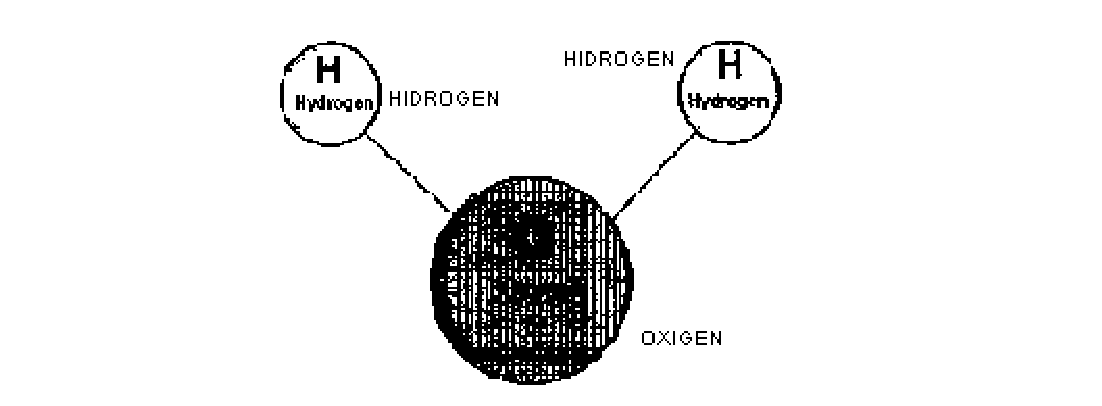
\includegraphics[width=1\linewidth]{img/molecule1.eps}
\caption{Water is two elements combined. A molecule of water consist of two 
atoms of hydrogen and one of oxygen.}
\label{fig:molecule1}
\end{subfigure}%
\hfill
\begin{subfigure}{.45\textwidth}
\centering
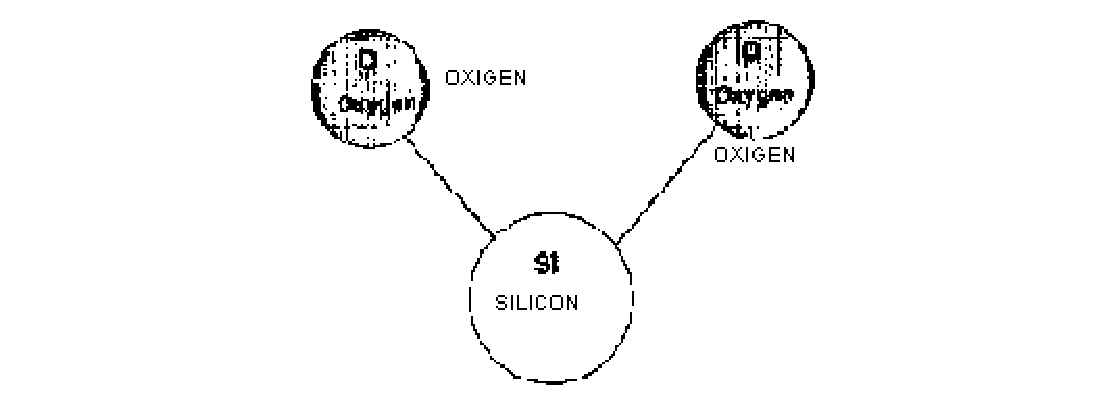
\includegraphics[width=1\linewidth]{img/molecule2.eps}
\caption{A molecule of the compound silica (sand) has two atoms of oxygen and 
one of silicon}
\label{fig:molecule2}
\end{subfigure}
\caption{Different molecules.}
\label{fig:molecules}
\end{figure}
%-------------------------------------------------------------------------------
Ceramic raw materials are usually in the form of oxides: an oxide is a compound 
that includes oxygen (O). Minerals are compounds.
%-------------------------------------------------------------------------------
\subsection{Solid, Liquid, Gas}
Solid, liquid and gas are the three states of matter. Most materials can exist 
in all of these states, depending on their temperature. A familiar example is 
water, which is solid below 0\degree C, liquid from 0\degree C to 100\degree C, 
and gas above 100\degree C.

Making glaze depends on mixing solids together, applying them on a pot and then 
changing them to liquid in the kiln. Some of the glaze materials also become 
gas during firing and leave the glaze. On cooling, the glaze again becomes 
solid.
%-------------------------------------------------------------------------------
\subsection{Mixture}
A mixture is a physical, not chemical, combination of compounds (and sometimes 
elements) and each compound remains chemically unchanged in the mixture. Air is 
a mixture of oxygen, carbon dioxide, nitrogen and other gases. A glaze made of 
feldspar, quartz and lime is prepared by combining the compounds as a mixture, 
but during firing a chemical combination takes place and the fired glaze 
becomes a compound.
%-------------------------------------------------------------------------------
\subsection{Chemical Symbols}
There are about 100 elements, and each of these has a name and a chemical 
symbol, which is used as an abbreviation of its name. Some of these symbols are 
the same as the first letters of the English name, but some are not!

For example:
%-------------------------------------------------------------------------------
\begin{itemize}
\item Oxygen is \ce{O}
\item Hydrogen is \ce{H}
\item Silicon is \ce{Si}
\item Alumina is \ce{Al}
\item Sodium is \ce{Na}
\item Lead is \ce{Pb}
\end{itemize}
%-------------------------------------------------------------------------------
Compounds are written in a similar way with capital letters marking the 
individual elements: for example, water \ce{H2O} and salt is \ce{NaCl}

The small number ``2'' in \ce{H2O} indicates that there are two atoms of 
hydrogen 
for each atom of oxygen in water. If there is no number, it is understood that 
there is only one atom--so salt is one atom of sodium and one atom of chlorine.

The formulas of complex ceramic materials are written as compounds of oxides 
with a raised period (\ce{*}) between them to show they are chemically combined. For 
example potash feldspar is written:

\ce{K2O*Al2O3*6SiO2}

In the appendix the chemical formulas of other materials are listed.
%-------------------------------------------------------------------------------
\subsection{Chemical Reactions}
The formation of clay from feldspar can be written in chemical symbols:

\ce{K2O*Al2O3*6SiO2 + H2O -> Al2O3*2SiO2*2H2O + K2O + SiO2}

$Feldspar + Water \rightarrow Clay + Potash + Silica$

All materials are built up of elements which are chemically bonded together. 
When heated to a high temperature, chemical bonds can break down and the 
material will change its properties. The production of quicklime by heating 
limestone to 900\degree C is an example of this:

\ce{CaCO3 -> CaO + CO2}

$Limestone + Quicklime \rightarrow Carbon~Dioxide$

Carbon dioxide \ce{(CO2)} goes into the air, and the remaining quicklime 
\ce{(CaO)} is slaked with water and can then be mixed with sand to form mortar 
for house construction. The mortar sets when the calcium oxide \ce{(CaO)} takes 
back carbon dioxide \ce{(CO2)} from the air and thereby regains the hardness of 
the original limestone \ce{(CaCO3)}:


\ce{CaO + Co2 -> CaCO3}

$Soft~mortar + Air \rightarrow Set~mortar$
%-------------------------------------------------------------------------------
\subsection{Solutions and Suspensions}
%-------------------------------------------------------------------------------
\subsubsection{Solution}
A solution is a mixture of molecules. For example, sugar completely dissolves 
in water: the separate particles consist of molecules of sugar and water. Sugar 
and water remain a solution until the water evaporates.

The higher the temperature of the liquid, the more solid material can dissolve 
in the liquid. When no more solid can be dissolved the solution is called 
``saturated''.
%-------------------------------------------------------------------------------
\subsubsection{Suspension}
In a suspension the particles are bigger than molecules. A mixture of clay and 
water is a suspension. The clay particles are not changed by the water, and 
after some time the clay will settle at the bottom of the vessel. The clay is 
insoluble in water.
%-------------------------------------------------------------------------------
\subsection{Crystal Structures}
If we heat water to 90\degree C and add salt \ce{(NaCl)}, it will become 
dissolved in the water. If we continue to add salt until no more salt can be 
dissolved, the suspension is saturated with salt. If we let the solution cool 
to room temperature (20\degree C) the water can hold much less salt in 
solution, with the result that some of the salt will separate in the form of 
salt crystals.

All minerals have the form of crystals. When the water cools, the excess salt 
molecules start to combine with one another in regular patterns like small 
building blocks. The way the salt molecules connect to one another is very 
orderly and produces a cube-shaped crystal. Different materials will produce 
crystals of different shapes. The shape of a mineral's crystal is used to 
identify it.
%-------------------------------------------------------------------------------
\begin{figure}[htbp!]
\centering
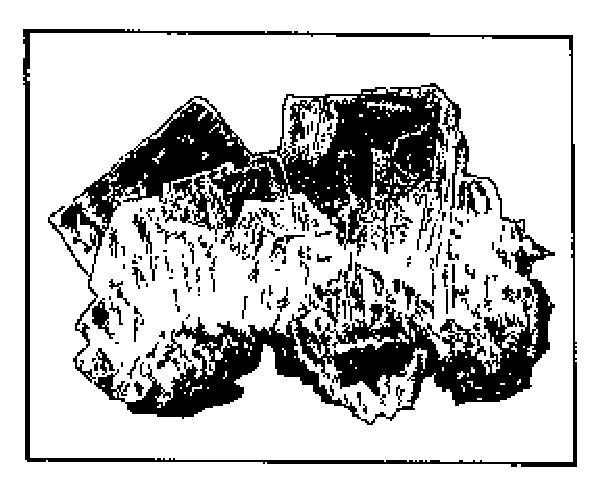
\includegraphics[width=0.5\linewidth]{img/salt.eps}
\caption{The cubic shape of a salt crystal.}
\label{fig:salt}
\end{figure}
%-------------------------------------------------------------------------------
\section{Glaze Structure}
Glaze is similar to glass. Making glazes is confusing because there are so many 
raw materials that can be used. However, all of these raw materials can be 
broken down into three categories:
%-------------------------------------------------------------------------------
\begin{itemize}
\item Flux
\item Glass former
\item Stabilizer
\end{itemize}
%-------------------------------------------------------------------------------
All glazes require these three components. The main glass former is silica, the 
main stabilizer is kaolin, and the rest of the glaze is composed of one or more 
fluxes.
%-------------------------------------------------------------------------------
\subsection{Glass Structure}
Silica \ce{(SiO2)} alone will make an excellent glaze if it is fired to its 
melting point (1715\degree C). Since this temperature is too high for ordinary 
kilns, other materials are added to lower the melting point of silica. Quartz 
is a crystalline form of silica found in nature. If a glaze forms quartz 
crystals when it cools, it will not be transparent, since light is refracted in 
many different directions by the crystal faces. Because glass or glaze is not 
usually crystalline, this does not happen.

A glaze or glass is a mixture of compounds that melts when heated. The melted 
liquid glass is like a solution. When the liquid cools, crystals start to form 
in a similar way as in a salt solution. However, the liquid glaze is very 
viscous (meaning sticky and semifluid) and the molecules cannot easily move 
around to form a regular crystalline pattern. So normally no crystals form 
during cooling, and the glaze remains clear like a liquid.

Glaze is, therefore, like a solid solution and is sometimes called a 
supercooled liquid.
%-------------------------------------------------------------------------------
\subsection{Fluxes}
Fluxes are the materials which lower the melting point of a glaze. They can be 
called melters.

Silica melts by itself but at a very high temperature. Therefore it needs 
additions of flux to make a practical glaze. The most common flux for 
temperatures below 1100\degree C is lead oxide \ce{(PbO)}, but since it is 
poisonous it is no longer used in modern crockery glazes. Another powerful flux 
is boron or boric oxide, \ce{B2O3}, which is not poisonous and is used in 
glazes in 
the form of borax or boric acid. There are many other fluxes which contribute 
various properties of hardness, opacity, color response etc.

Fluxes are also called basic oxides or network modifiers.
%-------------------------------------------------------------------------------
\subsection{Glass Formers}
Silica forms the main part of all glazes and is called a glass-former. The 
other glass-former is boron. Silica and boron are the building blocks of a 
glass or glaze. Other materials are only used to modify their behavior in the 
glaze.

Titanium oxide \ce{(TiO2)}, tin oxide \ce{(SnO2)} and zirconium oxide 
\ce{(ZrO2)} also belong to this group. Sometimes they are called the acidic 
oxides or network former, or the acid portion of the glaze.
%-------------------------------------------------------------------------------
\subsection{Stabilizers}
Aluminum oxide, \ce{Al2O3}, is added to make the melted glaze stiffer, so that 
it will not run off the pots during firing. It is called a stabilizer. Other 
words for stabilizer are: amphoteric, neutral or intermediate oxide.

Aluminum oxide has a high melting point and will increase the melting point of 
the glaze. It is usually added to the glaze as kaolin (china clay).

(Boron is termed a stabilizer in the USA but a glass former in Europe.)
%-------------------------------------------------------------------------------
\section{Effect of Heat}
As heat is increased, the molecules in the glaze move faster, resulting in 
drying, sintering, melting and gas escape. All of these effects occur when the 
glaze molecules move so fast that they start to break down, releasing some of 
their atoms and combining with other molecules to form the glaze.
%-------------------------------------------------------------------------------
\subsection{Drying}
When the powdered glaze on the surface of the ceramic ware is heated, the water 
evaporates above 100\degree C (no matter how dry the glaze seems to be, there 
will 
always be some water remaining in it). The glaze layer should be as dry as 
possible before setting in the kiln. If the glaze layer dries too fast when 
firing starts, it may crack. This can cause crawling of the glaze after it 
melts.
%-------------------------------------------------------------------------------
\subsection{Sintering, Melting, Gas Escape}
%-------------------------------------------------------------------------------
\subsubsection{Sintering}
As the temperature rises above 600\degree C, the sintering of the glaze powder 
starts. 
Sintering also takes place in the clay at this temperature. Sintering means 
that the glaze (or clay) particles start to stick to one another where they 
touch. The finer the glaze particles are ground, the earlier the sintering will 
start and the stronger the bond will become.
%-------------------------------------------------------------------------------
\begin{figure}[htbp!]
  \centering
  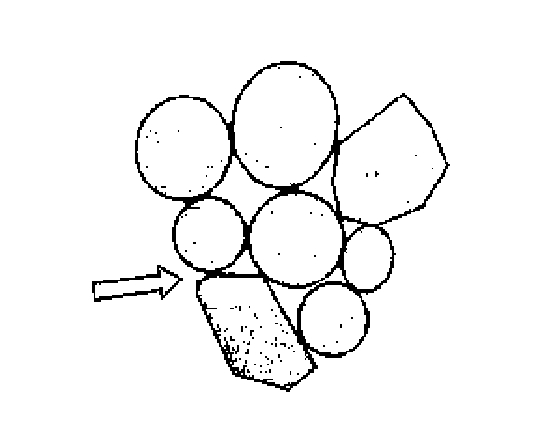
\includegraphics[width=0.5\linewidth]{img/sintering.eps}
  \caption{The glaze particles are enraged many thousand times showing 
  sintering in a glaze heated to 600\degree C. At the points of contact (arrow) 
  a weak 
  bond is formed.}
  \label{fig:sintering}
\end{figure}
%-------------------------------------------------------------------------------
\subsubsection{Fusion}
As the temperature rises further, the most fusible (easy melting) materials in 
the glaze start to melt. This is celled fusion. The refractory (hard melting) 
particles are surrounded by the liquid materials and are slowly included in the 
liquid.

The temperature at which melting starts depends on the materials in the glaze. 
Silica alone melts at 1715\degree C, but with additions of other materials the 
melting point will go down. Aluminum oxide \ce{(Al2O3)} melts at 2050\degree C 
and calcium oxide \ce{(CaO)} at 2570\degree C, but a mixture of 62\% 
silica, 14.75\% aluminum oxide and 23.25\% lime melts at only 1170\degree 
C. A mixture which has a lower melting point than any of the single materials 
in the mixture is called an eutectic.

A mixture with many different materials will form eutectics (and will melt) at 
a lower temperature. Fine grinding of the glaze materials and prolonged firing 
time above the sintering temperature will also lower the melting point.

When fusion starts, the compounds also start to change. The chemically bonded 
water in clay has already been released. Around 900\degree C, limestone 
\ce{(CaCO3)} releases carbon dioxide \ce{(CO2)} and so do other materials 
containing carbonates, like barium carbonate \ce{(BaCO3)}. Gases of sulfates, 
oxides etc. are also released both from the glaze and from the body. These 
gases have to pass through the glaze layer. This action mixes the glaze, 
helping it to become homogeneous.

In the beginning the melted glaze is very stiff (high viscosity), but as the 
temperature keeps rising the glaze becomes more fluid and, when watching the 
melting glaze surface through a spyhole in the kiln, bubbling or even boiling 
can be seen. When the glaze reaches its maturing temperature, the reactions 
stop and the glaze becomes smooth.
%-------------------------------------------------------------------------------
\begin{figure}[htbp!]
\centering
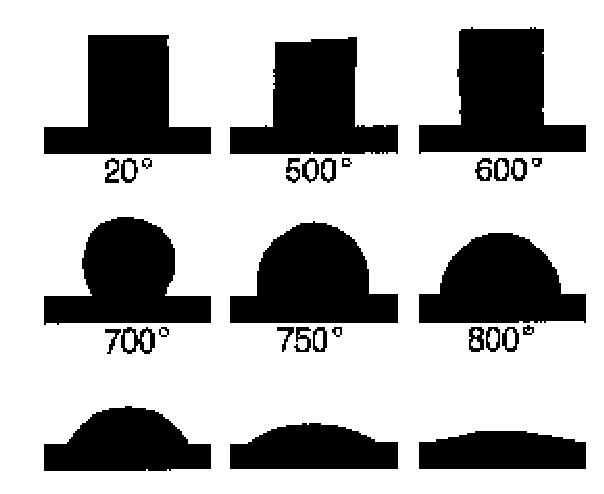
\includegraphics[width=0.5\linewidth]{img/fusion.eps}
\caption{A cube of glaze is gradually heated up to 1000\degree C. At 500\degree 
C the glaze shrinks slightly (sintering), but at 600\degree C it swells as 
gases develop. Melting starts before 700\degree C and is completed at 
1000\degree C.}
\label{fig:fusion}
\end{figure}
%-------------------------------------------------------------------------------
\subsection{Materials Which Increase or Decrease Melting Point}
\label{sec:meltingpointsec}
Table~\ref{tab:glazephysicalcharacteristics} shows the oxides according to 
their influence on 
melting temperature.
%------------------------------------------------------------------------------
\begin{center}
        \renewcommand{\arraystretch}{1.5}
        \begin{table}\centering
\begin{tabular}{|c|c|c|c|c|c|}\hline
    \multicolumn{2}{|c}{\textbf{Melting Point}}
    &\multicolumn{2}{|c|}{\textbf{Viscosity}}
    &\multicolumn{2}{c|}{\textbf{Surface Tension}}
\\\hline\hline
%------------------------------------------------------------------------------
\textbf{Oxide}&\textbf{Effect}&\textbf{Oxide}&\textbf{Effect}&\textbf{Oxide}
&\textbf{Effect}\\\hline\hline
%------------------------------------------------------------------------------
\ce{Al2O3}&Raise&\ce{Al2O3}&Increase&\ce{Al2O3}&Increase\\\hline
%------------------------------------------------------------------------------
\ce{SiO2}&-&\ce{ZrO2}&-&\ce{ZrO2}&-\\\hline
%------------------------------------------------------------------------------
\ce{MgO}&-&\ce{SiO2}&-&\ce{ZnO}&-\\\hline
%------------------------------------------------------------------------------
\ce{Cr2O3}&-&\ce{Cr2O3}&-&\ce{CaO}&-\\\hline
%------------------------------------------------------------------------------
\ce{SnO2}&-&\ce{NiO}&-&\ce{SnO2}&-\\\hline
%------------------------------------------------------------------------------
\ce{ZrO2}&-&\ce{Fe2O3}&-&\ce{Cr2O3}&-\\\hline
%------------------------------------------------------------------------------
\ce{NiO}&-&\ce{TiO2}&-&\ce{NiO}&-\\\hline
%------------------------------------------------------------------------------
\ce{Fe2O3}&-&\ce{CaO}&-&\ce{BaO}&-\\\hline
%------------------------------------------------------------------------------
\ce{TiO2}&-&\ce{MgO}&-& \ce{SrO}&-\\\hline
%------------------------------------------------------------------------------
\ce{CaO}&-&\ce{ZnO}&-&\ce{Fe2O3}&-\\\hline
%------------------------------------------------------------------------------
\ce{ZnO}&-&\ce{SrO}&-&\ce{SiO2}&-\\\hline
%------------------------------------------------------------------------------
\ce{BaO}&-&\ce{BaO}&-&\ce{TiO2}&-\\\hline
%------------------------------------------------------------------------------
\ce{FeO}&-&\ce{CoO}&-&\ce{Li2O}&-\\\hline
%------------------------------------------------------------------------------
\ce{CoO}&-&\ce{MnO}&-&\ce{Na2O}&-\\\hline
%------------------------------------------------------------------------------
\ce{CuO}&-&\ce{PbO}&-&\ce{K2O}&-\\\hline
%------------------------------------------------------------------------------
\ce{MnO}&-&\ce{K2O}&-&\ce{B2O3}&-\\\hline
%------------------------------------------------------------------------------
\ce{PbO}&-&\ce{Na2O}&-&\ce{PbO}&Decrease\\\hline
%------------------------------------------------------------------------------
\ce{B2O}3&-&\ce{B2O3}&-&&\\\hline
%------------------------------------------------------------------------------
\ce{Na2O}&-&\ce{Li2O}&Decrease&&\\\hline
%------------------------------------------------------------------------------
\ce{K2O}&-&&&&\\\hline
%------------------------------------------------------------------------------
\ce{Li2O}&Lower&&&&\\\hline
%------------------------------------------------------------------------------
\end{tabular}
\caption{Materials which affect physical characteristics of a 
glaze. Note this scale is not linear and depends on variables like firing 
temperature, amount of oxide in the glaze, and (for surface tension) the glaze 
viscosity.}
\label{tab:glazephysicalcharacteristics}
\end{table}
\end{center}
%------------------------------------------------------------------------------
\section{Melted Glaze Behavior}
\subsection{Fluid State}
The fluid state of the glaze should be maintained long enough to allow all 
bubbles time to escape, so the glaze layer can heal over the holes left by the 
escaping bubbles. If a glaze tends to produce pinholes and craters, it can be 
given a soaking period (keeping the kiln at maturing temperature for some time) 
or the firing temperature can be raised in order to make the glaze more fluid 
(reduce viscosity).

If the glaze is too fluid, it will run off the pot or the fluid glaze will soak 
into a porous body leaving matt, dry spots on the surface.

Table~\ref{tab:glazephysicalcharacteristics} shows materials which increase or 
decrease viscosity:
%------------------------------------------------------------------------------
\subsection{Surface Tensions}
\label{sec:surfacetension}
To understand surface tension, fill a glass with water to the rim and look at 
the water surface. The middle of the water surface will be higher than the rim, 
but the water will not run over. The surface tension of the water holds it as 
if it were held by a plastic membrane.

A small amount of water forms a spherical drop. Larger amounts of water flatten 
the spherical form because the force of gravity increases with the weight of 
water. The fluid glaze behaves in a similar manner, and if the surface tension 
of the fluid glaze is too high the glaze will pull itself into small islands, 
leaving the clay body uncovered. This is called crawling.

Different oxides have different effects on glaze surface tension, as 
table~\ref{tab:glazephysicalcharacteristics} illustrates.

Increasing temperature lowers the surface tension as 
figure~\ref{fig:fusion} illustrates. At 800\degree C the glaze forms a half 
globe but at 1000\degree C it has completely flattened out.
%-------------------------------------------------------------------------------
\begin{figure}[htbp!]
  \centering
  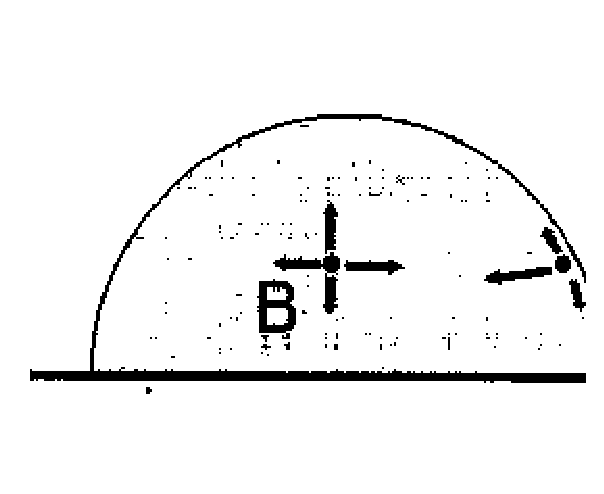
\includegraphics[width=0.5\linewidth]{img/surfacetension.eps}
  \caption{Surface tension is created by the difference of forces acting on 
  water 
    in the center (B) and at the surface (A). A water particle at B has forces 
    of traction of the water around it evenly distributed. But at A the force 
    is 
    mainly directed away from the surface. This difference causes water to form 
    itself ion spherical drops.}
  \label{fig:surfacetensionimage}
\end{figure}
%------------------------------------------------------------------------------
\subsection{Crawling}
Crawling is caused by two factors:
%------------------------------------------------------------------------------
\begin{itemize}
\item high surface tension of the glaze
\item difficulty for the glaze to stick to the body
\end{itemize}
%------------------------------------------------------------------------------
If the body surface is greasy or dusty the problem is aggravated. Crawling may 
also happen if the glaze layer cracks before it is sintered. This happens if 
the glaze contains a high amount of clay or has been ground for too long in the 
ball mill. The surface tension will then pull the glaze away from the cracks.
%-------------------------------------------------------------------------------
\begin{figure}[htbp!]
  \centering
  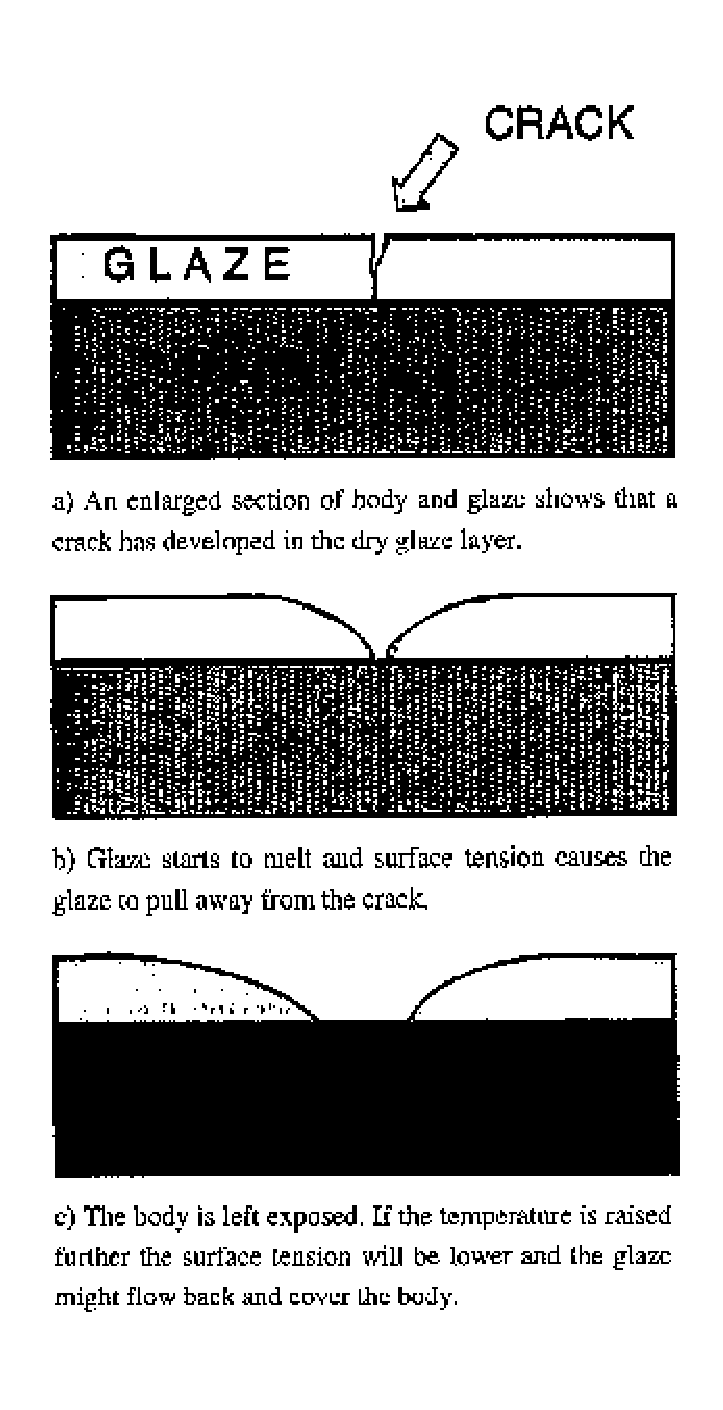
\includegraphics[width=0.5\linewidth]{img/crawling.eps}
  \caption{Crawling.}
  \label{fig:crawling}
\end{figure}
%-------------------------------------------------------------------------------
\subsection{Craters and Pinholes}
The lower the surface tension, the shinier the surface of the glaze becomes and 
the easier it is for the glaze to heal over craters, bubbles and pinholes.

Interesting effects can be obtained by applying glazes with different surface 
tensions on top of each other.

Surface tension, viscosity and melting temperature are interrelated, so when 
replacing materials all three will be affected.
%-------------------------------------------------------------------------------
\section{Interface between Glaze and Body}
During firing the glaze interacts with the clay body. Some of the glaze will 
sink into the body and some of the body material will mix with the glaze so 
that an intermediate layer is formed between the body and the glaze. This layer 
bonds the clay and glaze together. It is called the glaze/body interface or 
``buffer'' layer.
%-------------------------------------------------------------------------------
\subsection{Effects of Interface}
Some of the coloring oxides in the body may enter the glaze and change its 
colon The higher the firing temperature the stronger the interface layer. The 
interface layer produces a strong bond between glaze and body that reduces the 
tendency to craze or peel.

Glazing on greenware (raw glazing or green glazing or single firing) promotes 
interaction between body and glaze. If too much of the glaze's flux combines 
with the refractory materials in the body, the glaze may become matt or dry.
%-------------------------------------------------------------------------------
\begin{figure}[htbp!]
  \centering
  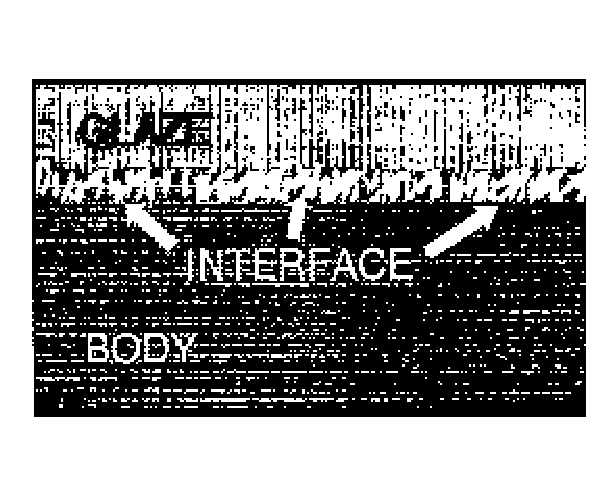
\includegraphics[width=0.8\linewidth]{img/interface.eps}
  \caption{Interface layer created during firing by mixing of materials in the 
  body and the glaze.}
  \label{fig:interface}
\end{figure}
%-------------------------------------------------------------------------------
\section{Cooling and Crystal Formation}
Glaze or glass is called a supercooled liquid because, during cooling, crystals 
have no time to form in the rather sticky mass, and glass by definition does 
not contain crystals. But some matt glazes and opaque glazes depend on the 
formation of crystals. For these, cooling should be slow to allow the crystals 
to grow. \ce{ZnO}, \ce{BaO}, and \ce{TiO2} are used for making matt glazes, but 
if cooling is rapid the glaze will become glossy instead of matt.

To avoid crystal formation, glossy transparent glazes should be cooled quickly 
after the maturing temperature has been reached.
%-------------------------------------------------------------------------------
\section{Transparency and Opacity}
Transparency is the property of allowing light to pass through the glaze to-the 
clay below. Transparent glazes may be colorless or have color in them - 
transparent blue, green, brown etc. It is necessary to use transparent glazes 
in combination with underglaze decoration. Transparent glazes are always shiny.

Opacity is the property of not allowing light to pass through the glaze. 
Colorless opaque glazes usually look white or gray. When coloring oxides are 
added, they can be any possible colors. They generally are used with overglaze 
or on-glaze.

It is possible to make glazes with every degree of transparency or opacity, 
such as semitransparent or semiopaque.
%-------------------------------------------------------------------------------
\begin{figure}[htbp!]
  \centering
  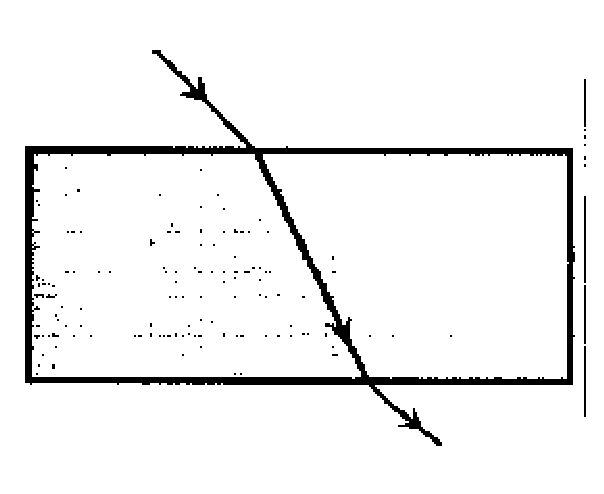
\includegraphics[width=0.5\linewidth]{img/transparency.eps}
  \caption{Section of a window glass. A beam of light passes through it - it is 
  transparent. The lights dissection is slightly bent when passing from one 
  medium (air) to another (glass). This is called refraction.}
  \label{fig:transparency}
\end{figure}
%-------------------------------------------------------------------------------
\subsection{Refraction of Light}
Transparency and opacity are determined by the glaze's ability to transmit 
light. When light strikes a transparent glaze, most of it passes through the 
glaze layer to the clay underneath, and the color we see is determined by the 
color of the clay. Thus, a transparent glaze on a brown clay body will look 
brown whereas the same glaze on a white clay body will look white. If the 
transparent glaze is colored, the clay body color will be changed by the fact 
that the glaze is green or blue, etc.
%-------------------------------------------------------------------------------
\begin{figure}[htbp!]
  \centering
  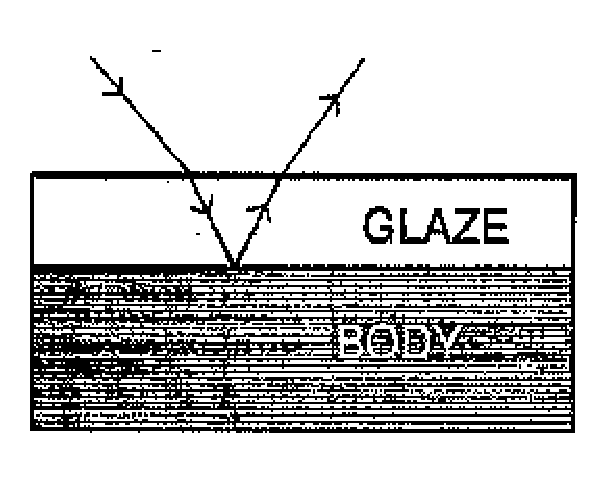
\includegraphics[width=0.5\linewidth]{img/reflecting.eps}
  \caption{A transparent glaze reflects the color of the underlying body.}
  \label{fig:reflecting}
\end{figure}
%-------------------------------------------------------------------------------
Opaque glazes have a large number of particles in them that reflect light, 
without allowing it to pass through the glaze. So we are not able to see 
through the glaze. Thus what we observe is only the surface of the glaze, which 
is not affected by the color of the clay underneath.

Semitransparent glazes have smaller numbers of light-reflecting particles, so 
they look cloudy or milky, and their color will be affected by the clay color 
underneath.

Transparent glazes can be made opaque by the addition of opacifiers, which are 
finely ground particles that do not enter into the melting of the glaze. These 
particles stay suspended in the glaze and reflect light. This is similar to 
mixing clay with water, which makes the water opaque.

Opaque glazes cannot be made transparent without changing their formula (unless 
they are transparent glazes with opacifier added).

The causes of opacity in glazes can be divided into 4 groups:
%-------------------------------------------------------------------------------
\begin{enumerate}
\item Presence of very fine particles, which do not dissolve in the glaze melt. 
The light going through the glaze is scattered by the fine particles. Tin oxide 
\ce{(SnO2)} and zircon \ce{(ZrSiO4)} are used for this.
\item Crystals formed in the glaze during cooling will scatter the light, 
causing opacity. Titanium dioxide \ce{(TiO2)} recrystallizes if the cooling is 
slow and can make glazes opaque.
\item Opacity is also caused when two melting phases of the glaze do not mix. 
The light will be scattered when it passes through the border between the two 
different melts. This takes place in boron glazes and with calcium phosphate 
(bone ash).
\item Gas bubbles scatter the light and produce opacity. This type of opacity 
is difficult to control and the method is not recommended.
\end{enumerate}
%-------------------------------------------------------------------------------
In practice, a combination of the four methods is used. For example, an opaque 
glaze can be made with boron and additions of lime, zinc oxide and zircon.
%-------------------------------------------------------------------------------
\subsection{Materials Causing Opacity}
The best opacifier is tin oxide, which will make most glazes opaque in 
additions of up to 7\%. However, it is a very expensive material and today is 
only used for special high-cost products.

Commercially available opacifiers are based on zirconium silicate, prepared 
with other additions such as magnesia and zinc oxide. They are marketed under 
names such as ``zirconium opacifier'', ``zirconium silicate'', ``zinc zirconium 
silicate'' and ``magnesium zirconium silicate''. Most of these are added to 
glazes 
from 5 to 10\% and produce different results depending on the type of base 
glaze. They also vary widely in quality, and it is important to test them 
before ordering a large quantity. Zirconium opacifiers have the disadvantage of 
making glazes more refractory and often cause pinholing problems.

The main opacifiers are:
%-------------------------------------------------------------------------------
\begin{itemize}
\item Tin oxide, \ce{SnO2}
\item Zircon, zirconium silicate, \ce{ZrSiO4}
\item Titanium dioxide, \ce{TiO2}
\item Alumina, \ce{Al2O3} (high content in boron glazes will reduce opacity)
\item Calcium oxide, \ce{CaO} (improves opacity in boron glazes)
\item Zinc oxide, \ce{ZnO}
\item Calcium phosphate, bone ash, \ce{Ca3(PO4)2}
\end{itemize}
%-------------------------------------------------------------------------------
\subsection{Particle Size}
The finer the particle size of the opacifier, the better it works. Zircon is 
often included in the frit batch for greater opacity. In this way opacity is 
obtained with less zircon, thus reducing some of zircon's bad side effects like 
high viscosity and the tendency to cause pinholes. Unfortunately the addition 
of zircon to the frit increases its melting point, making it more difficult to 
run it off the frit kiln. It also increases the hardness of the frit so much 
that it may be difficult to grind it with ordinary pebbles and ball mill lining.

It is important to make sure that the opacifier is well dispersed in the glaze. 
The fine particles tend to lump together. This reduces the opacity effect. By 
ball milling the opacifier together with the glaze a good dispersion is assured.
%-------------------------------------------------------------------------------
\section{Shiny or Matt Glaze}
Glazes are also defined by the way they reflect light: they may be shiny or 
matt or in between.
%-------------------------------------------------------------------------------
\subsubsection{Shiny Glaze}
Shiny glazes are also known as ``glossy'' or ``bright''. They have the property 
of 
reflecting light like a mirror. They are best for utilitarian wares, sanitary 
ware and insulators, as they are easy to wash and do not scratch easily.
%-------------------------------------------------------------------------------
\begin{figure}[htbp!]
  \centering
  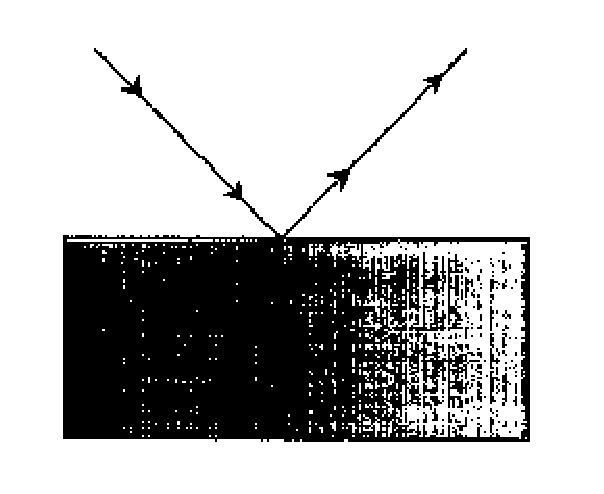
\includegraphics[width=0.5\linewidth]{img/glossyglaze.eps}
  \caption{A glossy glaze with a smooth surface reflects the light without 
  scattering it.}
  \label{fig:glossyglaze}
\end{figure}
%-------------------------------------------------------------------------------
\subsubsection{Matt Glaze}
Matt glazes are also known as ``dull'' or ``non-reflective''. Their surface can 
vary from smooth to very rough. They are useful for decorative wares and are 
very popular for floor tiles, which need to be beautiful but not slippery. The 
matt surface is not functional for dinnerware, because used with cutlery it 
makes an unpleasant sound and scratches easily.
%-------------------------------------------------------------------------------
\subsection{Materials Causing Mattness}
%-------------------------------------------------------------------------------
\subsubsection{Underfiring}
As glaze begins to melt, it becomes glassy. If the firing is stopped before the 
glaze is completely melted, even glossy glazes will appear matt. Often these 
underfired glazes will have other problems such as blisters and pinholes, but 
some glossy glazes make very good matt glazes if fired a few cones below their 
normal temperature. Similarly, adding refractory oxides to a glaze (such as 
china clay or calcium carbonate) will produce a matt glaze that really is just 
an underfired glossy glaze.
%-------------------------------------------------------------------------------
\subsubsection{Crystalline Matt}
Crystalline matt glazes develop small crystals which break up light (see 
Figure~\ref{fig:crystallinematt}). This type of matt glaze usually produces a 
more smooth surface than underfired matt glazes. Some matt glazes depend on 
slow cooling to have time for the crystals to develop.

Barium carbonate, zinc oxide, titanium dioxide, magnesium oxide and calcium 
oxide are the agents for crystal matt glazes.
%-------------------------------------------------------------------------------
\begin{figure}[htbp!]
  \centering
  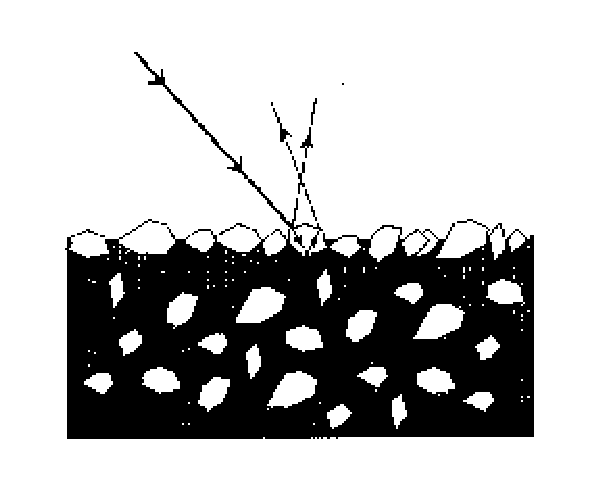
\includegraphics[width=0.5\linewidth]{img/crystallinematt.eps}
  \caption{Surface of crystal matt glaze enlarged several hundred times. 
    Crystals in the glaze scater the light by sending it in many different 
    directions.}
  \label{fig:crystallinematt}
\end{figure}
%-------------------------------------------------------------------------------%-------------------------------------------------------------------------------
\subsection{Other Causes}
Sometimes glazes that should be glossy will become matt. Some reasons 
are:
\begin{itemize}
\item Some of the flux materials may evaporate during firing.
\item Sulfates from fuel may settle on the surface of the glaze.
\item The glaze is applied too thin.
\item The glaze was not mixed sufficiently or not sieved finely enough.
\end{itemize}
%-------------------------------------------------------------------------------
\chapter{Obtaining Glaze Materials}
%-------------------------------------------------------------------------------
\section{Materials Suppliers}
In countries with large ceramics industries, there are suppliers that 
specialize in collecting and distributing raw materials. These may be mining 
companies that can supply specific items like clay and feldspar. If these can 
be obtained directly, it saves the costs of middlemen. However, these companies 
often deal only in large quantities. For the small producer, it is often best 
to get supplies from reliable distributors.
%-------------------------------------------------------------------------------
\subsection{Local Suppliers of Chemicals}
General chemical suppliers or pharmacies often have many of the necessary 
ingredients for glazes (which are often used in other industries). They are 
useful for obtaining small amounts of chemicals, but often their prices are 
high.
%-------------------------------------------------------------------------------
\subsection{Suppliers of Other Industries}
Glaze materials are often available from other types of suppliers. For example, 
agricultural suppliers can provide calcined limestone. Paint industries use 
materials such as iron oxide and opacifiers.
%-------------------------------------------------------------------------------
\subsection{Imported Materials}
Imported materials should only be considered if there are no local sources, as 
they are expensive and often customs and import regulations make it difficult 
or impossible for the small producer to obtain them. On the other hand, it is 
often worth paying the additional price, if it makes possible production of 
special glazes or decoration effects that are in demand in the market.

In Thailand, for example, where there is a large export market for decorative 
ceramics, many producers import clay, glazes and overglazes from Japan. Their 
profit comes from cheap labor and high value added.
%-------------------------------------------------------------------------------
\section{Materials from Natural Sources}
Small producers can mine their own materials if these are available in the 
area. Historically, pottery centers located themselves where the necessary clay 
and glaze materials were available. Where stoneware clay and high temperatures 
are used, it is possible to make glazes from low-temperature clay alone. 
Generally, stoneware glazes are made from the basic ingredients of feldspar, 
quartz, limestone and clay, which are quite common. Wood ash is another common 
base for high temperature glazes. The process of mining, selecting and grinding 
is quite time-consuming, and with the advent of modern transportation it is 
often cheaper to purchase materials from suppliers.

In Nepal, we developed low-temperature glazes based on borax, which must be 
imported. The bulk of the glaze is composed of local materials such as rice 
husk ash (for silica), limestone and local clay, which are all easy to get and 
cheap.
%-------------------------------------------------------------------------------
\subsection{Crystal Rocks}
%-------------------------------------------------------------------------------
\subsubsection{Igneous Rocks}
When the young earth slowly started to cool, different minerals formed crystals 
in the mass of molten rocks (magma). A variety of crystalline rocks were formed 
differing in composition according to their locality. For example, the igneous 
rock called basalt was created at a great depth and contains little feldspar 
compared to granite, which formed near the surface.

If rock cools very slowly, crystals have time to grow large, whereas rapid 
cooling produces small crystals. This process is still going on today where 
movement in the crust of the earth causes deep layers of molten materials to 
rise to the surface. An erupting volcano lets out hot magma, which cools 
quickly. The resulting volcanic rocks have microscopic-size crystals, since the 
rapid cooling allows little time for crystals to grow.

The most common crystal rocks used in glazes are feldspar and quartz. If a 
piece of granite is picked up and broken in two, the fresh faces of the stone 
will show a shiny surface and the crystals of the different minerals can be 
identified. The black crystals are mica or tourmaline. The yellow, white or red 
colored crystals with a pearly shine are different types of feldspar. The clear 
colorless crystals are quartz. The weathered surface of the granite will most 
probably show a rough surface with many holes, where the soluble feldspar 
crystals have been washed away by rain, whereas the less soluble crystals of 
mica and quartz remain. Coarse granite (known as pegmatite) often breaks up in 
weathering, leaving large pieces of quartz and feldspar lying on the ground. 
These can be collected, ground and used in glazes.
%-------------------------------------------------------------------------------
\subsubsection{Volcanic Rocks}
These are rocks formed by the action of volcanoes, often in the form of molten 
lava that flows out of the volcano. The crystals in the rock are extremely 
small because the lava cooled very fast. Lava is essentially a glaze and can be 
used as the basis of high temperature glazes.
%-------------------------------------------------------------------------------
\subsection{Sedimentary Rocks}
Sedimentary rocks are made of materials produced by the crumbling of old rocks. 
All rocks eventually break up in the course of time when exposed to weather, 
and the broken-up rock particles are carried away by water. These particles of 
clay and sand are transported to lower lying areas or to the sea where they 
settle one layer upon the other. In the span of millions of years, the growing 
weight of sediments causes the deeper layers to compact and gradually turn into 
rocks, called sedimentary rocks. Much later, the movement of landmasses 
sometimes turns the whole area upside down, so that the old sea floor, with its 
sedimentary rocks, becomes a new range of mountains.

The upper part of new mountains consists of sedimentary rocks resting on deeply 
set igneous rocks. Sedimentary rocks like sandstone, shale and slate can often 
be recognized by their layered structure. Limestone is a sedimentary rock 
created by the skeletons of billions of small animals that lived in the ancient 
seas. Gypsum is formed by chemical sedimentation in areas where seawater 
evaporates on a large scale. This produces a high concentration of gypsum which 
forms crystals like the formation of salt crystals in a glass of salty water.

For the glazemaker, sedimentary shale can be a source of glaze. At high 
temperatures, shale melts and with a few additions will produce glazes that are 
usually brown. Although shale often does not slake in water, it can be ground 
in a pan mill and used in glaze.
%-------------------------------------------------------------------------------
\begin{figure}[htbp!]
  \centering
  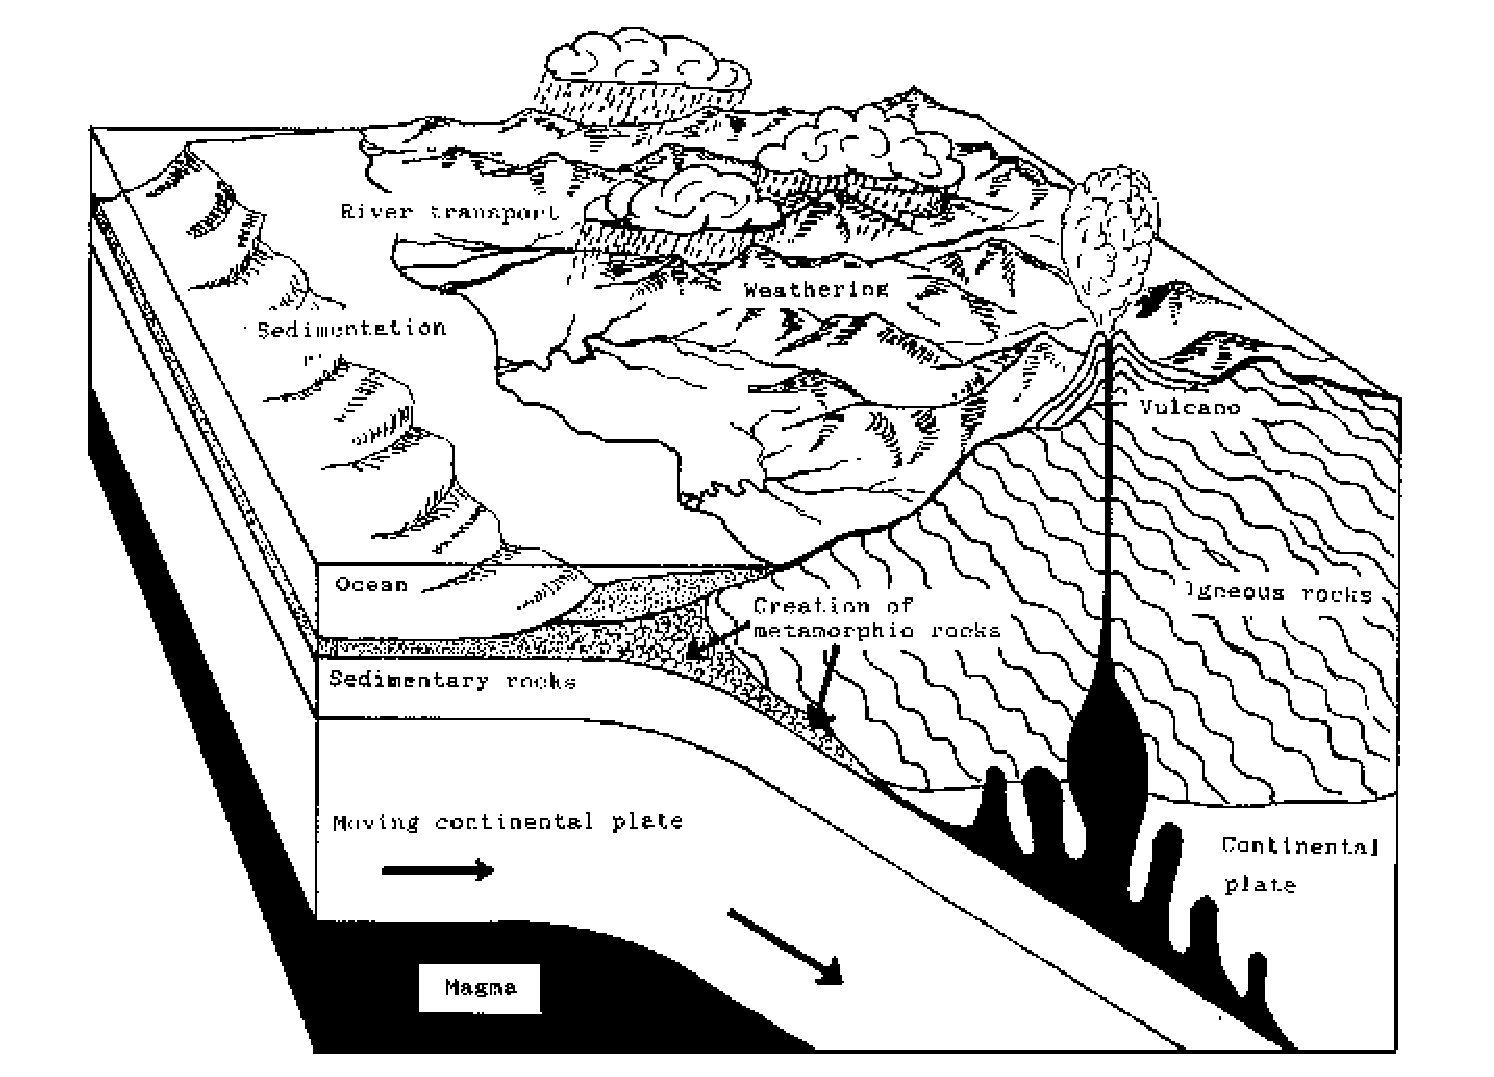
\includegraphics[width=0.9\linewidth]{img/continentalplate.eps}
  \caption{A cutout of a section of the crust of the earth shows a continental 
  plate moving under another. The friction of the plates generates heat, which 
  melts rocks and feeds a volcano. Rain falls and old rocks are weathered and 
  washed to the sea creating new layers of sediments. Later the sediments are 
  compressed into rocks.}
  \label{fig:continentalplate}
\end{figure}
%-------------------------------------------------------------------------------%-------------------------------------------------------------------------------
\subsection{Metamorphic Rocks}
Igneous and sedimentary rocks are sometimes changed into new forms by high 
temperature and pressure. Marble is an example of a metamorphic rock formed 
from the sedimentary rock limestone.
%-------------------------------------------------------------------------------%-------------------------------------------------------------------------------
\subsection{How to Get Information}
\subsubsection{Local Authorities}
First of all, information about the geology and the minerals of the region 
should be gathered from local authorities, like industrial development 
organizations, agricultural institutions, National Geological Institutes or 
mining corporations. They may have little information and the authorities may 
even say that no materials are available in the region. However, that is often 
not true and should not keep anybody from looking on his own.
%-------------------------------------------------------------------------------%-------------------------------------------------------------------------------
\subsubsection{Practical People}
It is worth talking to people who make water wells, and builders of dams and 
roads. They sometimes have useful information about the minerals of the region. 
Farmers in the area will know about the upper layers of soil on their fields 
and about local rocks. Sometimes glaze minerals are used for other purposes, 
like whitewashing houses or medicine.

The best source of information is often other potters.
%-------------------------------------------------------------------------------%-------------------------------------------------------------------------------
\subsection{Looking for Minerals}
Good places to look for minerals are in riverbeds, where many different types 
of rocks will wash down from the mountains above. Although most of these may 
not be useful, it is often possible to find quartz and feldspar. Any rock with 
an unusual color is worth testing. Rocks that are unusually heavy may contain 
metallic oxides. For the potter, however, there are few rocks that are directly 
useful, other than quartz, feldspar and limestone, and some of the volcanic 
rocks.

Other minerals that are useful in glazes are sodium and potassium compounds, 
which sometimes form on the edge of lakes, particularly in desert areas. These 
usually look like a white powder and are soluble in water.
%-------------------------------------------------------------------------------%-------------------------------------------------------------------------------
\subsection{Testing}
To begin with, the most useful test is to take a small sample of the material, 
place it in a clay bowl and fire it in a regular glaze firing. This will 
indicate if it melts or not. If it melts, it certainly can be used in a glaze. 
Materials that do not melt should not be automatically rejected, as many useful 
glaze materials (such as calcium carbonate and quartz) only melt when combined 
with other materials. The simplest way to find out if they are of use is to 
make a line blend of one of your standard glazes, combined with the unknown 
material.

Rock minerals can be identified by their crystal shape, color, specific gravity 
and hardness. If you are seriously looking for rock minerals there are good 
books presenting most common minerals with color photos.

Mohs' scale of hardness is based on the hardness of 10 different minerals. 
Window glass and a penknife are about 5.5 and a metal file about 6.5.

Two materials have the same hardness if they cannot scratch each other. Quartz 
can scratch feldspar but not topaz. In the field a piece of glass and a 
penknife are used to find out if the hardness of a rock is higher or lower than 
5.5.

If a testing laboratory is available, samples can be sent there for chemical 
analysis. This is usually expensive but may be helpful if the material looks 
useful after firing.
%------------------------------------------------------------------------------
\begin{center}
        \renewcommand{\arraystretch}{1.5}
          \begin{table}\centering
    \begin{tabular}{|c|c|}\hline
      \textbf{Mineral}&\textbf{Hardness}\\\hline\hline
      %------------------------------------------------------------------------------
      Talc&1\\\hline
      %------------------------------------------------------------------------------
      Gypsum&2\\\hline
      %------------------------------------------------------------------------------
      Calcite&3\\\hline
      %------------------------------------------------------------------------------
      Fluorspar&4\\\hline
      %------------------------------------------------------------------------------
      Apatite&5\\\hline
      %------------------------------------------------------------------------------
      Orthoclase feldspar&6\\\hline
      %------------------------------------------------------------------------------
      Quartz&7\\\hline
      %------------------------------------------------------------------------------
      Topaz&8\\\hline
      %------------------------------------------------------------------------------
      Corundum&9\\\hline
      %------------------------------------------------------------------------------
      Diamond&10\\\hline
    \end{tabular}
    \caption{Mohs' Scale of Hardness.}
    \label{tab:mohs}
  \end{table}
\end{center}
%------------------------------------------------------------------------------
\section{Other Sources of Materials}
Recycled materials are often useful in glazes. These may be by-products from 
other industries, such as rice husk ash or bone meal, or waste materials. Some 
other sources of useful materials are discussed below.
%------------------------------------------------------------------------------
\subsection{Metallic Oxides}
Metallic oxides are used as coloring agents in glazes. Commonly available are:

Iron oxide, which can be obtained by scraping rust from old steel. It is often 
possible to get this from paint and hardware suppliers, who use "red oxide" for 
coloring paint and cement.

Manganese dioxide, which is the main ingredient in torch batteries (the black 
substance which can be removed from old batteries).

Copper oxide, which can be collected from makers of copper pots. The oxide is 
the black powder that forms on the surface of copper when it is heated. Another 
way is to fire copper wire in the kiln and to use the resulting black copper 
oxide.
%------------------------------------------------------------------------------
\subsection{Ashes}
Wood ashes are used as the basis for high temperature glazes, since they 
contain sodium, potassium, silica and other ingredients. Early glazes were 
often simple mixtures of wood ash and clay. Most wood ash is suitable for this 
purpose, but each type of wood will produce different characteristics and will 
have a different melting point. So it is important to have a consistent supply. 
Ash must be sieved to remove unburned material and is usually washed in water 
and dried before use. If it is not washed it contains more fluxes but they are 
soluble and make the glaze slip caustic.

At cone 8 to 11, a good starting point is 2 parts ash, 2 parts feldspar and 1 
part clay. Ash glazes have general limits as shown in 
table~\ref{tab:limits}.

Rice husk ash contains more than 90\% silica, so it can be used instead of 
quartz in many cases. For accuracy, it should be burned white--if there is 
much black carbon in it, it will make calculations incorrect. 

In Appendix~\ref{sec:appendix_composition} the chemical composition of 
different ashes is given.
%------------------------------------------------------------------------------
\begin{center}
        \renewcommand{\arraystretch}{1.5}
          \begin{table}\centering
    \begin{tabular}{|c|c|}\hline
      \textbf{Material}&\textbf{Percent}\\\hline\hline
      %------------------------------------------------------------------------------
      Ash&20--70\%\\\hline
      %------------------------------------------------------------------------------
      Feldspar&20--70\%\\\hline
      %------------------------------------------------------------------------------
      Whiting&5--20\%\\\hline
      %------------------------------------------------------------------------------
      Flint&15--25\%\\\hline
      %------------------------------------------------------------------------------
      Clay&5--20\%\\\hline
    \end{tabular}
    \caption{Limits of material content in glazes.}
    \label{tab:limits}
  \end{table}
\end{center}
%------------------------------------------------------------------------------
\section{Storing, Packaging, and Labeling}
If you use local materials, they will change from time to time. For this 
reason, it is best to store as much material as possible and to check each new 
batch by trying it in a standard glaze. For example, feldspar tends to be 
variable and, as the mine is used, the chemical composition will change. 
Suppliers of feldspar usually keep several large storage areas of material from 
different parts of the mine. In order to keep it uniform, they mix the 
different feldspars together when supplying.

Some materials are damaged by water. Borax, boric acid, soda ash and plaster of 
parts should all be kept in a dry place. In particular, soda ash absorbs water 
(up to 7\% after one year, 11\% after two years) and will thereafter no longer 
be effective as a slip deflocculant; and plaster will not set correctly after 
damp storage.

When you get local materials, each batch should be kept separately and labeled 
with date and source. It is often a good idea to purchase more material when 
your old supply is about 50\% finished and to test it to see if it is the same 
or not. If it is not greatly different, the new material can be mixed with the 
old and your glaze will not change unexpectedly.

A good labeling system is very important, as most glaze chemicals look rather 
alike. Never depend on your memory - keep a permanent label on the bag or jar 
of material. Additionally, if you order bags of material from a supplier, ask 
him to label the outside of the bag, and also to put a label inside the bag as 
labels are often lost in shipping.
%------------------------------------------------------------------------------
\chapter{Frits and Fritmaking}
\label{sec:frits}
Most low-temperature glazes require fluxes that are either poisonous (lead) or 
water-soluble (sodium and potassium). Traditionally, these materials were used 
raw, but this is not satisfactory for modern potters. Raw lead is poisonous and 
sodium/potassium are water-soluble. Borax is sometimes used raw in glazes, but 
these glazes cannot be stored for a long time, as the borax will go into 
solution or form crystals.

The principle of fritmaking is very simple: molecules of poisonous or soluble 
fluxes should be chemically combined with glass-making materials to eliminate 
these undesirable characteristics.

A frit is a combination of a flux or several fluxes (lead, borax, boric acid, 
potassium carbonate) that is combined with other insoluble materials (quartz, 
feldspar, lime etc.), melted in a kiln to form an insoluble glass, and ground 
to be used as the base for making glazes. (Many low temperature glazes are 
simply 90\% frit and 10\% china clay).

Fritmaking is not usually practical for the small producer, as it takes time 
and requires a special kiln and a ball mill for grinding. On the other hand, if 
reliable frits are not commercially available, the potter may have to produce 
his own. Frit glazes are more expensive than raw glazes, but their convenience 
usually makes up for the additional cost.

There are many different commercially available frits, all designed for 
different temperatures, surface qualities, coefficients of expansion, and color 
responses. The potter trying to decide which frit to use must depend on the 
supplier, as formulas are usually kept secret. Suppliers will give advice on 
which frit is best for the potter's purpose. There are two main types of frit:
%-------------------------------------------------------------------------------
\begin{itemize}
\item Lead frits

These are all designed to provide lead in a nontoxic form. Lead oxide is 
combined with other materials to give desired properties of surface, opacity, 
and color response. The standard lead frit is called lead bisilicate and is 
simply a combination of lead oxide and silica, which combines the lead in an 
insoluble form. This can be used as the base for a large variety of lead glazes.

Other frits used commonly in the tableware industry are called 
lead-borosilicate frits, which combine the desirable properties of both lead 
and boron and are generally safer to use.

\textbf{Warning:} Lead frits can still be poisonous, and glazes made from them 
can be poisonous if they are not combined with sufficient silica to combine 
with all the lead molecules.

\item Leadless frits

These are based on boron compounds, again combined with other materials. 
Because glazes compounded with lead are difficult to control for lead release, 
leadless frits are recommended for small producers.
\end{itemize}
%-------------------------------------------------------------------------------
\section{Why Make Frits?}
Frit making is only suggested if reliable commercial sources are not available. 
Often frit manufacturers are not interested in supplying small amounts. 
Dishonest frit manufacturers sometimes sell bad batches of frit to small 
producers. Even though frit making is complicated, the small producer who makes 
his own frits at least has the process under his own control.

Raw borax glazes can be used, but they must be used immediately after mixing or 
problems will result from the soluble borax. This may be satisfactory for art 
pottery but, if consistent results are needed, it is better to use fritted 
glazes.

Similarly, raw lead glazes are widely used. This is a danger for the workers, 
who will eventually develop lead poisoning unless they take extreme care in 
handling the glaze. Modern industries never use raw lead glazes, and 
industrialized countries all have severe restrictions on the use of lead in 
glazes. In developing countries, workers in industry suffer from lead 
poisoning, and it is the responsibility of the industrialist alone to take care 
of the workers' health. As lead poisoning takes several years to develop, many 
factory owners do not understand the seriousness of the problem and continue to 
harm their workers. 

\textbf{It can take up to 20 years to develop symptoms of lead poisoning.}
%-------------------------------------------------------------------------------
\section{Frit Production}
\subsection{Frit composition}
All the soluble materials are included in the frit batch along with silica, in 
order to form a glass when fired in the frit kiln. Other ma" serials may be 
included for modifying the frit or helping to melt it.

The main frit raw materials are:
%-------------------------------------------------------------------------------
\begin{itemize}
\item Silica sand, \ce{SiO2}
\item Rice husk ash, almost 95\% \ce{SiO2}
\item Borax, or sodium borate, \ce{Na2B4O7*10H2O}
\item Boric acid, \ce{H3BO3}
\item Limestone, \ce{CaCO3}
\item Feldspar, soda and/or potash, \ce{K2O , Na2O*Al2O3*6SiO2}
\item Clay, \ce{Al2O3*2SiO2}
\item Zinc oxide, \ce{ZnO}
\item Zircon, \ce{ZrSiO4} (opacifier)
\item Red lead oxide, \ce{Pb3O4}
\item Other materials like talc, barium carbonate and bone ash may be added.
\end{itemize}
%-------------------------------------------------------------------------------
In order to have a frit with low viscosity that easily runs out of the kiln, 
the clay or alumina of the glaze is not added to the frit. However, in order to 
make the ingredients insoluble, 2--3\% kaolin should be included in the frit.
%-------------------------------------------------------------------------------
\subsection{Workflow}
The work flow for frit production is shown in figure~\ref{fig:fritworkflow}. It 
is better economy to prepare large frit batches when firing a continuous-type 
frit kiln.
%-------------------------------------------------------------------------------
\begin{figure}[htbp!]
  \centering
  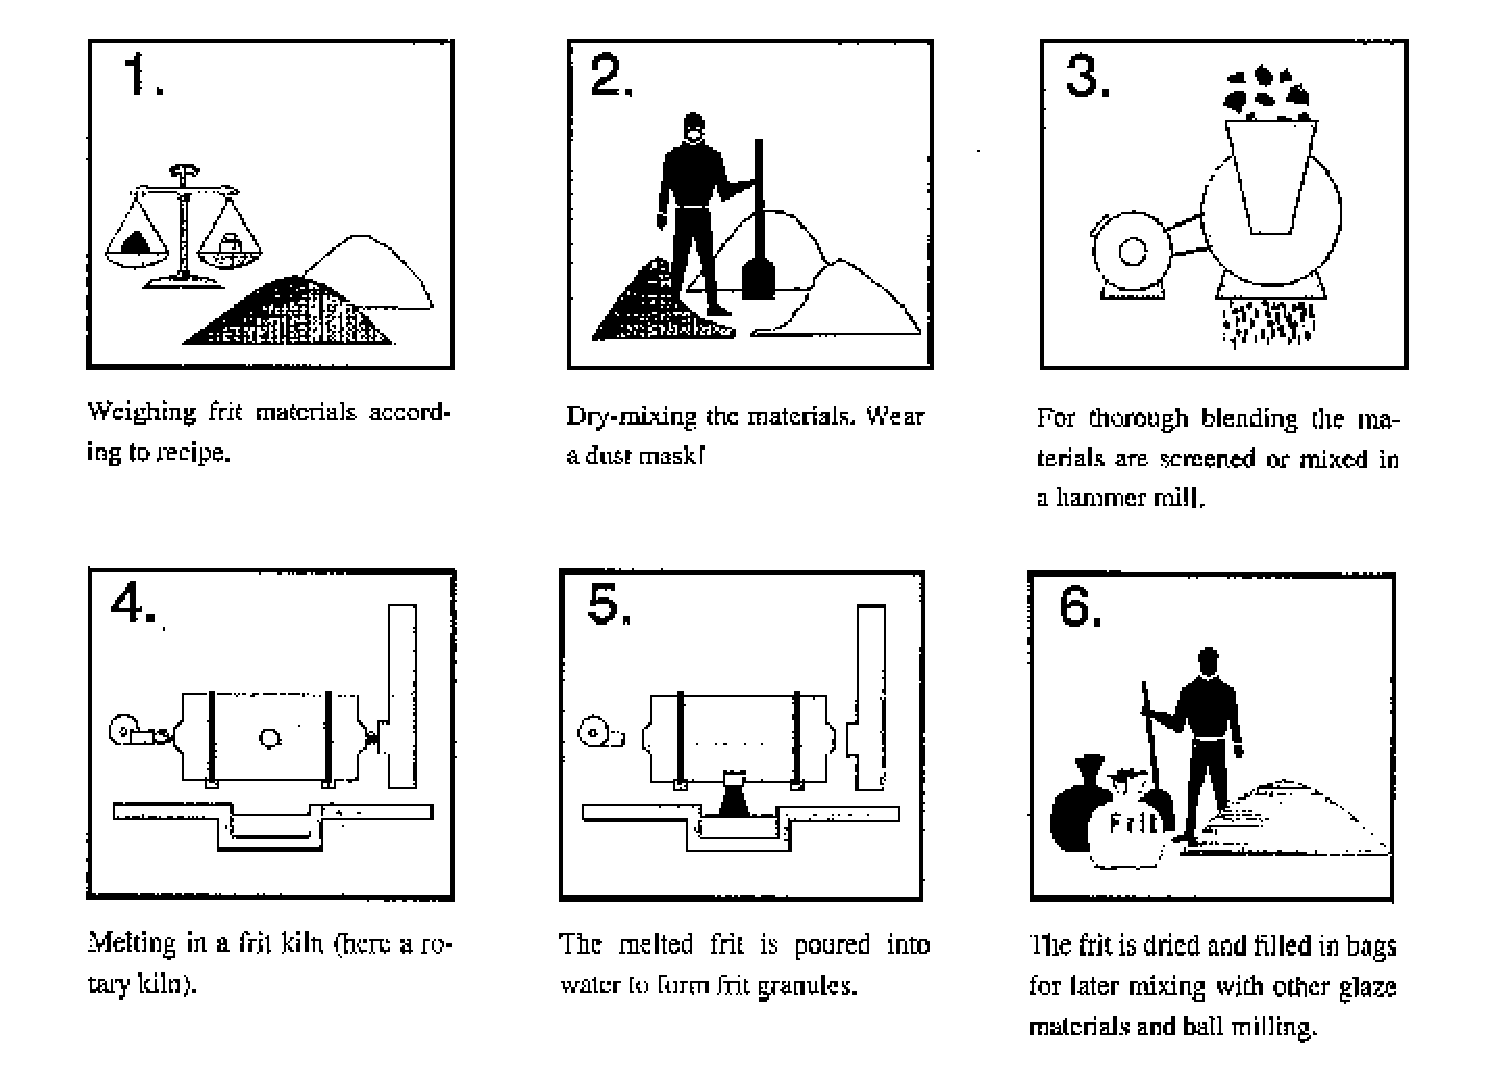
\includegraphics[width=0.8\linewidth]{img/fritworkflow.eps}
  \caption{Work flow of frit production.}
  \label{fig:fritworkflow}
\end{figure}
%-------------------------------------------------------------------------------
\begin{enumerate}
\item Prepare materials

All materials for frit need to be clean, dry and ground to pass through a 
60--100-mesh sieve. The finer the material, the easier it will be to melt it. 
If rice husk ash is used as the source of silica, it should be well-burned to a 
white color, so that unnecessary carbon is not introduced. If there is a large 
amount of black carbon, this will decrease the amount of silica available. The 
content of carbon in rice husk ash may vary more than 30\% from batch to batch.

If materials are wet, they should be dried completely so that the weight of 
water is not included in the recipe. In frit calculations, the loss on ignition 
needs to be included to account for loss of material during firing.

\item Blend materials

Weigh the materials accurately and blend them together dry. WEAR A DUST MASK! 
Small amounts can be mixed by hand in a bucket, and larger amounts can be mixed 
with a shovel on a clean cement floor. After mixing the frit materials they are 
screened through a 16-mesh sieve (mosquito net) to ensure thorough blending or 
the materials are run through a hammer mill.

\item Melt the frit in a kiln

There are many different systems for melting frit. In each system, the 
principle is to thoroughly melt the frit until all ingredient! are combined. 
Most frit is melted at 1150\degree C to 1250\degree C.

\item Check the frit

A sample of molten frit should be taken and examined to see if the melt is 
complete The frit should be uniform, without particle! of unmelted material.

With continuous frit kilns, the rate of feeding raw frit and the speed of the 
melted frit must be adjusted so that all the material melts completely and has 
time to mix' properly.

\item Quench the frit in cold water

The molten frit is poured into cold water, which ``shatters'' it into small 
pieces that can easily be ground. With continuous melting and discharging it is 
necessary to let fresh cold water run continuously.

\item Grind the frit

If the frit is quenched correctly, it will be easy to put it directly into a 
ball mill and grind it until it can be passed through a 100-mesh sieve. The 
granulated frit may be first dried and then stored in bags until it is needed 
for glaze making. Then it is ball-milled together with clay and other glaze 
materials. Alternatively, the still wet frit is ball-milled first.

\item Sieve the wet frit

When the frit is removed from the ball mill, it should be sieved through 100 
mesh to remove any large particles that were not ground.

\item Dry the frit

The wet frit is settled, excess water is poured off, and the remaining frit can 
be spread out to dry, either in the sun or in a dryer.

\item Test the frit

Each batch of frit should be tested for correctness. The simplest way is to 
fire it in a kiln on a specially made flow tester, along with a sample of 
correct frit. If the frit flows evenly to the control sample, it will probably 
be correct but should be double-checked by trying it in a standard glaze.

Additionally, the frit should be tested for solubility in water. A sample 
amount is boiled in water for several hours, then allowed to sit for 2 weeks. 
If crystals do not form during this time, the frit can be considered stable. If 
crystals form, it means that there is not enough silica/alumina in the frit and 
the composition will need to be changed. 

The causes of crystal formation could also be with the frit firing, e.g. 
overcharging, too short a firing time and improper mixing.

The finished tested frit may be sold to other ceramics producers either as a 
milled powder or in granular form.
%-------------------------------------------------------------------------------
\end{enumerate}
%-------------------------------------------------------------------------------
\section{Frit Kilns}
There are many different kinds of frit kilns, which are selected according to 
the amount of frit that needs to be regularly produced.

Normally, each type of frit--transparent, opaque, lead--requires a separate 
kiln to prevent contamination. When one kiln is used for several frits, it must 
be cleaned out before each different batch by melting frit in it to remove most 
of the old batch. This contaminated frit is then kept separately, to be used as 
``clean-out'' frit before changing to different compositions.
%-------------------------------------------------------------------------------
\subsection{Crucible Fritting}
Small amounts of frit for testing are easily made in a fireclay crucible. The 
crucible with frit is fired together in a glaze firing, which will melt the 
frit into a solid block of glass. After firing, the crucible is broken away 
from the frit and the frit can be crushed and ground. It is a good idea to 
first paint the inside of the crucible with china clay slip, as this will make 
it easier to separate the frit. 

\textbf{Note:} Frits containing boric acid often cannot be melted successfully 
this way, as the boric acid melts at a very low temperature and flows to the 
bottom before the rest of the ingredients melt. Frits with rice husk ash may 
also be difficult to melt in this way, because the upper layer of the frit 
melts first sealing off the frit mixture so that the carbon remaining in the 
ash cannot burn out. Carbon is highly refractory and it will prevent the frit 
from melting.

This is only suitable for test production and is not a safe method, since the 
pot often cracks, resulting in frit running out, destroying other ware, kiln 
furniture and the kiln lining.

\textbf{Caution:} Borax frits boil during melting with a great increase in 
volume. The crucible should be filled only half with frit, and a tile placed 
over the top to prevent boiling over.
%-------------------------------------------------------------------------------
\subsection{Crucible Kiln}
For fritting small amounts of frit a simple frit kiln is shown in 
figure~\ref{fig:cruciblekiln} It can be fitted with several crucibles arranged 
in a row for melting different frits at the same time. The crucibles can be 
loaded with raw frit from the top. The fuel economy of this type of kiln is 
less than for the other kilns.
%-------------------------------------------------------------------------------
\begin{figure}[htbp!]
  \centering
  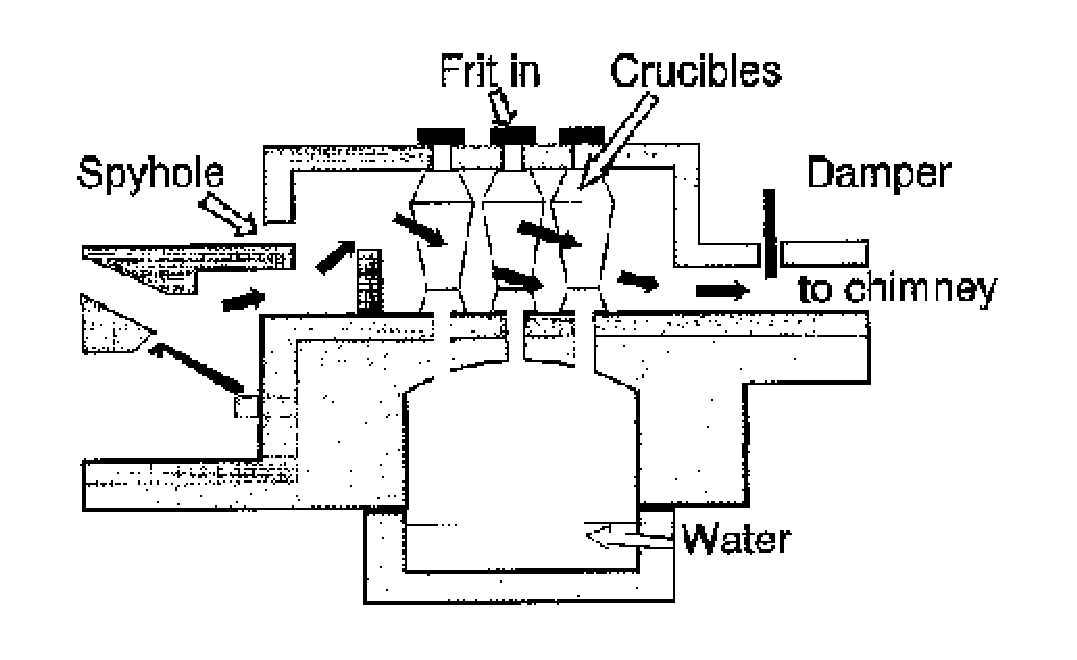
\includegraphics[width=0.8\linewidth]{img/cruciblekiln.eps}
  \caption{Coal-fired frit kiln with three crucibles.}
  \label{fig:cruciblekiln}
\end{figure}
%-------------------------------------------------------------------------------
\subsection{Open-Hearth Kilns}
Open hearth kilns consist of a tank made of firebricks, which is set in a 
crossdraft kiln. The kiln may be fired by coal, firewood, oil or gas. The hot 
flue gases heat the arch over the frit. The arch in turn heats the frit. In 
batch-type frit kilns, the frit melt is checked by drawing out some melted frit 
with an iron rod for inspection.

After the frit is completely melted, a hole at the bottom of the tank is opened 
and the frit flows out into cold water. Then another batch of frit may be 
charged from an opening in the arch.

The melting of several tonnes of frit may take 6--12 hours consuming 1--1.5 
tonne coal per 1 tonne melted frit.
%-------------------------------------------------------------------------------
\begin{figure}[htbp!]
  \centering
  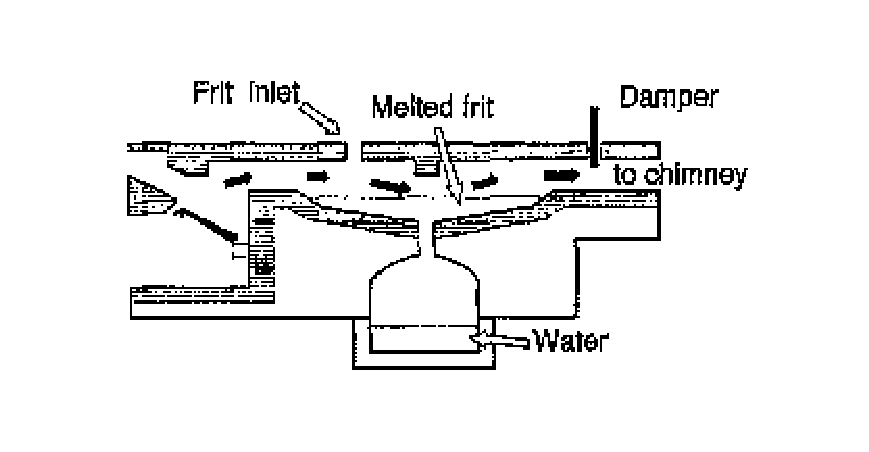
\includegraphics[width=0.8\linewidth]{img/openhearth.eps}
  \caption{Open-hearth frit kiln for coal firing.}
  \label{fig:openhearth}
\end{figure}
%-------------------------------------------------------------------------------
\subsection{Continuous Flow}
The continuous-flow frit kiln uses a kiln with a sloping floor, made of 
fireclay refractories. The raw frit is introduced at the upper end and, as it 
melts, it flows down while mixing to an exit chute by the burner and then into 
cold water. The kiln shown in figure~\ref{fig:continuousflow} was developed in 
Nepal. It uses a steam/kerosene burner, but any forced draft oil or gas burner 
can be used.

The rate of flow is controlled by introducing limited amounts of raw frit. Too 
much frit at one time may result in incomplete melting. If the frit runs very 
fast through the kiln, the low melting materials will not melt properly 
together with the silica. This may be a cause of water-soluble frit.

The frit can be slowed down in the kiln by making less of a slope and by 
putting some obstacles in the way (like kiln shelf supports).
%-------------------------------------------------------------------------------
\begin{figure}[htbp!]
  \centering
  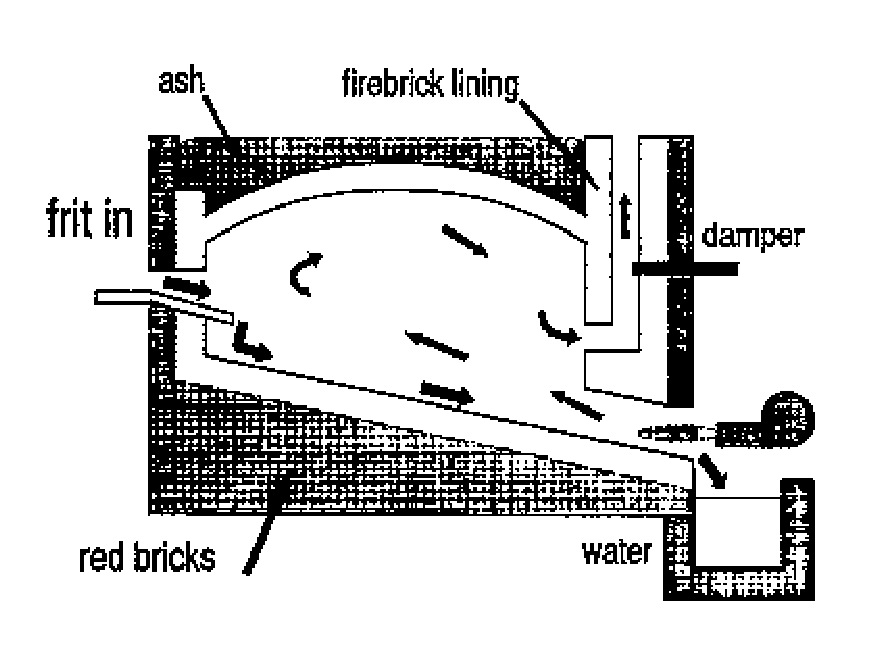
\includegraphics[width=0.8\linewidth]{img/continuousflow.eps}
  \caption{Side elevation of a continuous flow kiln.}
  \label{fig:continuousflow}
\end{figure}
%-------------------------------------------------------------------------------
\subsection{Rotary Frit Kiln}
Rotary frit kilns are large refractory-lined cylinders, which have a burner 
(gas or oil) that passes through them. The raw frit is introduced, and the kiln 
rotates full turns (or back and forth) as the frit melts. This has the double 
purpose of ensuring good mixing and of transferring the heat of the firebrick 
lining to the frit as this constantly moves over it. When the frit is 
completely melted, the kiln is turned so that the frit flows out through an 
opening into cold water.
%-------------------------------------------------------------------------------
\begin{figure}[htbp!]
  \centering
  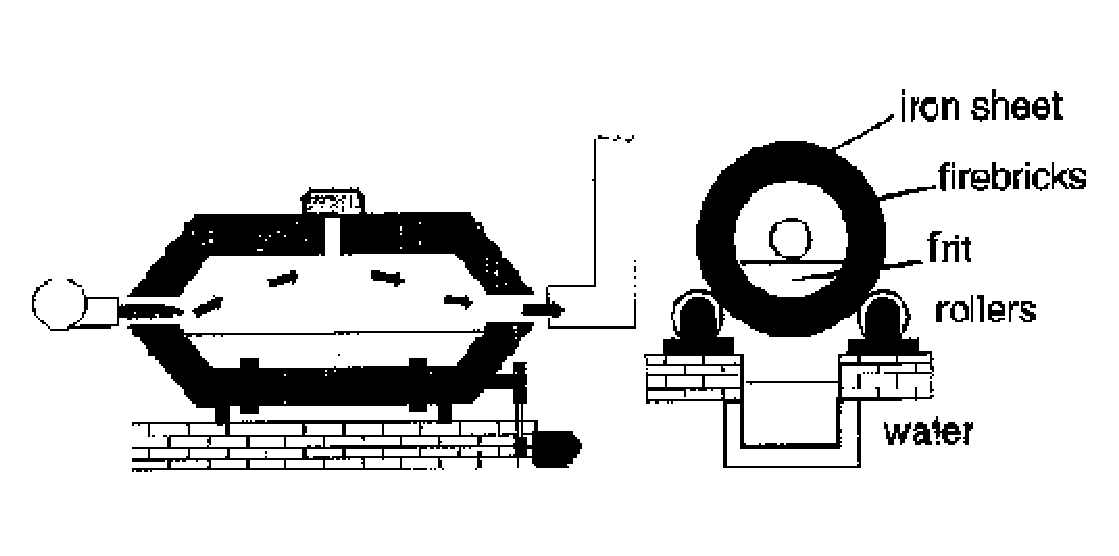
\includegraphics[width=0.8\linewidth]{img/rotarykiln.eps}
  \caption{Front and side elevation of a rotary frit kiln. It consists of a 
  firebrick-lined steel drum resting on rollers. It is gas-or oil-fired.}
  \label{fig:rotarykiln}
\end{figure}
%-------------------------------------------------------------------------------
\subsection{Fuel Economy}
If much frit is to be produced, fuel economy is an important factor. In 
general, the more frit that can be made at one time, the lower will be the fuel 
cost. In a continuous frit kiln, it takes several hours to heat the kiln 
sufficiently to melt the frit at maximum speed -this preheating period consumes 
a lot of fuel. It is best to fire several hundred kg of frit at the same time 
to reduce firing costs.

Frit industries generally use rotary kilns, as they are the most economical for 
long, continuous use. However, the continuous kiln developed in Nepal by the 
Ceramics Promotion Project compares favorably with standard fuel/frit ratios 
obtained with rotary furnaces.

Examples of fuel to melted frit ratios are shown in table~\ref{tab:fritratios}.
%------------------------------------------------------------------------------
\begin{landscape}
    \begin{table}\centering
\begin{center}
        \renewcommand{\arraystretch}{1.5}
    \begin{tabular}{|c|c|c|c|}\hline
      \textbf{Frit kiln type}&\textbf{Batch amount}&
      \textbf{Fritting time}&\textbf{kcal/kg melted frit}\\\hline\hline
      %------------------------------------------------------------------------------
      Open hearth coal&1--2 tones&6--12 hours&7500--11250\%\\\hline
      %------------------------------------------------------------------------------
      Continuous flow (Nepal)&1.5--2 tones&48 hours&5150\%\\\hline
      %------------------------------------------------------------------------------
      Rotary (India)&300 kg&2 hours&5700\%\\\hline
    \end{tabular}
    \caption{Fuel-to-melted frit ratios.}
    \label{tab:fritratios}
\end{center}
 \end{table}
\end{landscape}
%------------------------------------------------------------------------------
\chapter{Preparation of Glazes}
Glazes should be prepared in a systematic manner in order to prevent mistakes. 
Most problems with glazes come from simple things, like incorrect weighing, 
mistakes in identifying raw materials or not sieving the glaze correctly.

Glaze mistakes are expensive, as they can result in the loss of an entire 
kilnload. For this reason, it is important to have the right person in charge 
of making glazes--cleanliness, orderliness, careful record-keeping, and 
reliability are required.

Most small producers do not need a large variety of glazes -in fact, many use 
only one or two standard glazes and achieve variety by changing the colors, 
doubleglazing or using engobe decoration.

Designing a glaze is somewhat like choosing a paint in the paint store. First 
of all, you must decide if you want a glossy or matt surface, transparent or 
opaque. Then you can add different colors.
%-------------------------------------------------------------------------------
\subsection*{Base Glaze}
The base glaze is simply the combination of materials that melts at the desired 
temperature. It is either transparent or opaque, matt, semimatt, glossy etc. 
without any particular color.
%-------------------------------------------------------------------------------
\subsection*{Glaze Additions}
These are usually coloring oxides that are added to the glaze. In Nepal a glaze 
supplying system serving small producers was established. A base glaze was 
supplied in 5kg bags and 8 different colors were supplied in small bags that 
produced standard colors when added to 5 kg base glaze. The small bags contain 
coloring oxides mixed with a small amount of base glaze so the colors disperse 
more easily in the base glaze.
%-------------------------------------------------------------------------------
\section{Raw Materials Requirements}
Raw materials need to be as reliable as possible and always ground to the same 
mesh. If obtained from a glaze supplier, the materials are usually ground to at 
least 100 mesh. Because materials that are finely ground melt more easily, some 
ingredients may be as fine as 400 mesh. This is particularly true of 
quartz--200-mesh quartz will produce a different result than 400-mesh quartz.

When you get new raw materials, they always should be tested before using them 
in production. The best way is to try them in a standard glaze that you know 
well and to compare the results with the known glaze.
%-------------------------------------------------------------------------------
\section{Grinding Glaze Materials}
%-------------------------------------------------------------------------------
\subsection{Coarse Materials}
There are several steps in grinding glaze materials. Since many of them 
(feldspar, quartz, limestone) come as rocks, they first need to be reduced to 
pebble size. Feldspar and quartz rocks are first calcined to make them soft 
enough to crush. Calcining means firing to just above 600\degree C. This can be 
done 
in the cold spots of a biscuit firing or for large productions in a special 
kiln. Crushing of small amounts can be done with a hammer (use eye protection), 
and large amounts are usually done in a jaw crusher.
%-------------------------------------------------------------------------------
\subsection{Ball Milling}
\subsubsection{Ball Mill Operation}
Ball mills are used for fine grinding of ceramic materials. The material has to 
be reduced to sand size (2 mm or less) before grinding in a ball mill.

Some typical uses of ball mills are:
%-------------------------------------------------------------------------------
\begin{itemize}
\item grinding clay that does not easily slake
\item preparation of casting slips
\item grinding of body additions like feldspar, quartz and glass powder
\item grinding of frit granules grinding of glazes
\item grinding of engobes and terra sigillata
\item preparing color pigments for glaze, engobes or bodies.
\end{itemize}
%-------------------------------------------------------------------------------
There are two main types of mills:
%-------------------------------------------------------------------------------
\begin{itemize}
  \item Large mills with an axle system are called ball mills.
  \item Small mills are called pot mills or jar mills.
  
  These are usually small (up to 5--liter) porcelain jars or plastic jars, 
  which 
  rotate on two rubber-covered rollers.
\end{itemize}
%-------------------------------------------------------------------------------
\subsubsection{Conical ball mill}
For large production conical ball mills are used. Various sizes of pebbles are 
used and the material is fed from one end and discharged at the other. 
Variation of the centrifugal force caused by a conical 30\degree slope at the 
discharge side classifies both pebbles and material so only fine material is 
discharged.
%-------------------------------------------------------------------------------
\subsubsection{Vibro energy mill}
This is a new type of grinding machine consisting of cylindric grinding chamber 
suspended on springs and vibrated at high frequency with the help of an 
excentric mounted on an electric motor. The chamber is completely packed with 
very hard small cylinders between which the material is filled. The vibrations 
make the small cylinders grind against each other and the material to be 
ground. The vibrating mill is better at ultrafine grinding and is more 
energy-efficient than ball mills.
%-------------------------------------------------------------------------------
\subsubsection{Lining}
The grinding action takes place between the pebbles, and not between the 
pebbles and lining. Therefore a ball mill with a steel drum can work without a 
lining (except for white body, where rust particles will cause discoloration). 
Pebbles constantly falling on a steel drum make a lot of noise. A lining will 
reduce the noise and at the same time prolong the life of the steel. 
Traditionally, linings are made of porcelain or stoneware bricks set in a 
cement mortar, using high alumina cement and coarse silica sand. Common cement 
can be used if necessary but may cause pinhole problems in glazes. The bricks 
should be dense and vitreous. A porcelain body for lining bricks and pebbles 
(fire to 1250\degree C or higher) is shown in table~\ref{tab:liningbody}.

One type of brick is made concave to fit the curve of the drum and another type 
is made for the end walls of the drum.

Linings can be made from granite, quartzite or similar hard rocks (not 
limestone or marble). They are cut to shape and set in a high alumina cement 
mortar. They last far longer than porcelain bricks. Stoneware bricks can be 
used for the end walls, which are worn out more slowly.

Instead of a hard lining, thick rubber sheet glued to the inside makes a very 
long-lasting and quiet lining.
%------------------------------------------------------------------------------
\begin{center}
          \renewcommand{\arraystretch}{1.5}
  \begin{table}\centering
    \begin{tabular}{|c|c|}\hline
      \textbf{Ingredient}&\textbf{Percent}\\\hline\hline
      %------------------------------------------------------------------------------
      China clay&40\%\\\hline
      %------------------------------------------------------------------------------
      Quartz&25\%\\\hline
      %------------------------------------------------------------------------------
      Feldspar&30\%\\\hline
      %------------------------------------------------------------------------------
      Ball clay&5\%\\\hline
    \end{tabular}
    \caption{A porcelain body for lining bricks and pebbles.}
    \label{tab:liningbody}
  \end{table}
\end{center}
%------------------------------------------------------------------------------
\subsubsection{Pebbles}
Pebbles or balls can be made from vitreous clay bodies. However, it is often 
cheaper to collect stones of granite, quartz or quartzite along riverbeds. 
Flint, a variety of quartz, is excellent for pebbles. The hardness is tested 
with a penknife to make sure it is above 5.5 (see Mohs' scale, 
table~\ref{tab:mohs}). Pebbles of limestone are not satisfactory, as they 
contaminate the glaze. The shape should not be flat or elongated but spherical. 
(Cylinders of equal diameter and length are sometimes used to obtain particles 
with less variation in particle size.) Size should be between 2.5 and 5 cm in 
diameter.

Pebbles wear out, so occasionally take out all the pebbles for inspection. 
Those that are broken or flat should be discarded. In large mills, pebbles are 
removed when they are less than 2--3 cm. In small mills pebbles smaller than 
1.5--2 cm are discarded.

As the pebbles grind down, they contribute a small amount of material to the 
glaze. Usually this is not enough to make a difference in the glaze. However, 
if you have glaze problems that cannot be traced to any other cause, the ball 
mill pebbles should be checked.
%------------------------------------------------------------------------------
\subsubsection{Ball mill speed}
Grinding of material takes place between the pebbles of the ball mill as they 
roll down the slope of the cylinder. If the speed is too high, the grinding 
action stops because centrifugal force stops the pebbles from falling.

This happens when the cylinder is running at its critical speed. Critical speed 
is calculated from the inside diameter of the cylinder:

Critical~speed~in~rpm = $29.9/\sqrt{r}$ ($r$ = internal radius in meters)

The actual speed of the ball mill should be 60--80\% of critical speed. Small 
ball mills can be closer to 80\% and large ones closer to 60\% Appropriate 
speed can be read in figure~\ref{fig:ballmillspeed}.

The most efficient grinding is achieved when the pebbles roll as shown in the 
center ball mill of figure~\ref{fig:ballmillefficient}. The pebbles cascade in 
a steady stream, and grinding takes place between the pebbles. The speed of the 
ball mill at 80\% is too high. The pebbles have started to fall freely and this 
causes excessive wear as the pebbles hit one another and the lining.

Unfortunately it is not possible to look inside during milling, but if the 
pebbles make a low, rumbling sound the speed is correct. If they make a loud 
banging noise, the speed is too high or there is too much water, charge or 
pebbles in the mill. Porcelain jar mills crack if they run at too high a speed.
%-------------------------------------------------------------------------------
\begin{figure}[htbp!]
  \centering
  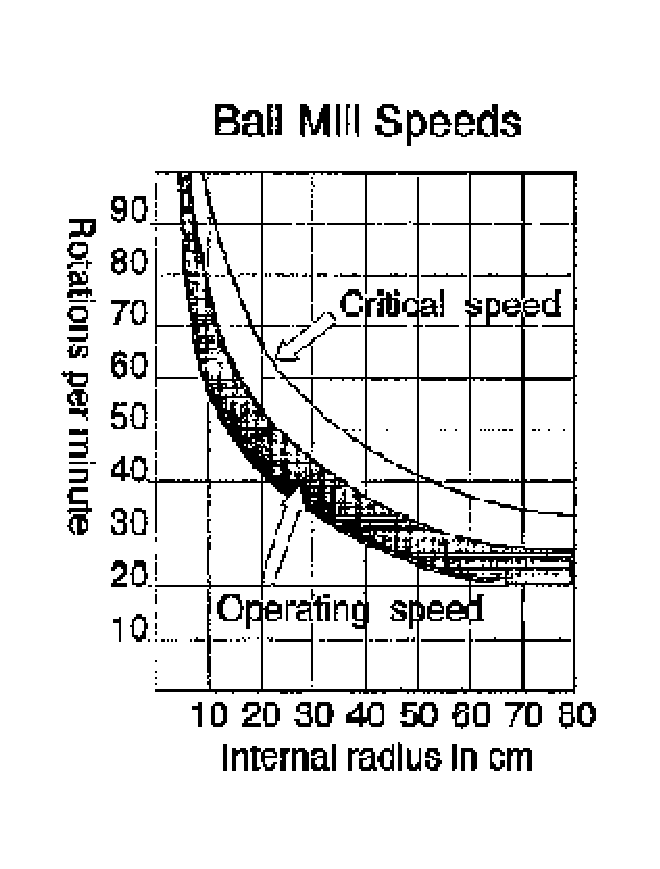
\includegraphics[width=0.8\linewidth]{img/ballmillspeed.eps}
  \caption{Graph of ball mill speeds.}
  \label{fig:ballmillspeed}
\end{figure}
%-------------------------------------------------------------------------------
\begin{figure}[htbp!]
  \centering
  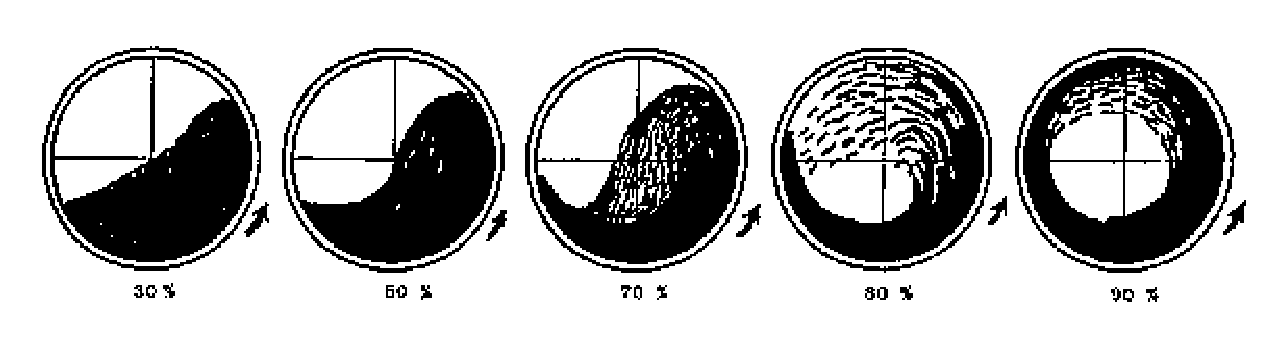
\includegraphics[width=0.8\linewidth]{img/ballmillefficient.eps}
  \caption{A cross section of a ball mill running at speeds from 30-90\% of 
  critical speed. At 30\% the grinding takes place mainly between pebbles and 
  lining, at 70\% a good cascading rolling produces efficient grinding, and at 
  90\% very little grinding takes place.}
  \label{fig:ballmillefficient}
\end{figure}
%-------------------------------------------------------------------------------
\subsubsection{Charge}
Table~\ref{tab:charge} shows the charge for a ball mill (by volume), with a 
speed of 60--80\% of critical speed.

When the mill is filled to maximum capacity, the speed should be closer to 60\% 
of critical speed. The water content should be enough to produce a thin slip. 
After filling, about 30\% of the volume should remain empty. If you measure all 
the materials separately, total volume may seem to be 85\% of ball mill 
capacity. However, since the water and material fill the spaces between the 
balls, this will still result in 30\% empty space.
%------------------------------------------------------------------------------
\begin{center}
          \renewcommand{\arraystretch}{1.5}
  \begin{table}\centering
    \begin{tabular}{|c|c|}\hline
      \textbf{Ingredient}&\textbf{Percent}\\\hline\hline
      %------------------------------------------------------------------------------
      Pebbles&45--55\%\\\hline
      %------------------------------------------------------------------------------
      Water&12--20\%\\\hline
      %------------------------------------------------------------------------------
      Material&20--25\%\\\hline
    \end{tabular}
    \caption{Proportions of charge in a ball mill at 60--80\% of critical 
      speed.}
    \label{tab:charge}
  \end{table}
\end{center}
%------------------------------------------------------------------------------
\subsubsection{Example}
A ball mill with new lining measures inside:

Width = $0.64 m$ 
Diameter = $0.445 m$

volume~of~ball~mill = $pi * r^2 * w$ (= \textbf{320 liters})

critical~speed = $29.9 / \sqrt{r}$ (= \textbf{58.2 RPM})

60--80\% of the critical speed = 31.7 RPM--42.3 RPM

A typical glaze has a density (specific gravity) of approximately 2.7. That 
means that the glaze charge should be 24-30 kg. For a breakdown of the charge, 
see table~\ref{tab:chargeexample}
%------------------------------------------------------------------------------
\begin{center}
          \renewcommand{\arraystretch}{1.5}
  \begin{table}\centering
    \begin{tabular}{|c|c|}\hline
      \textbf{Ingredient}&\textbf{Percent}\\\hline\hline
      %------------------------------------------------------------------------------
      Pebbles&144--176 liters\\\hline
      %------------------------------------------------------------------------------
      Water&38--64 liters\\\hline
      %------------------------------------------------------------------------------
      Material&64--80 liters\\\hline
    \end{tabular}
    \caption{Charge (by volume) of the example ball mill.}
    \label{tab:chargeexample}
  \end{table}
\end{center}
%------------------------------------------------------------------------------
\subsubsection{Ball Milling Time}
The time for ball milling varies with the hardness of materials. Soft materials 
such as frits may require only 2-3 hours, whereas hard materials like quartz 
can take 24 hours or more.

When you ball-mill standard materials, it is important to mill each batch for 
the same amount of time. For this reason, it is a wise investment to purchase a 
timer switch for the mill. This will avoid human errors. Too much ball milling 
can cause glaze crawling.
%------------------------------------------------------------------------------
\subsubsection{Operating Procedure}
Before each operation:
%------------------------------------------------------------------------------
\begin{itemize}
\item Check that the ball mill is clean inside.
\item Check that pebbles fill half of the ball mill -refill if necessary.
\item Fill in materials (20-25\% of mill volume).
\item Fill water until pebbles and material are just covered.
\item Be very careful about correct ball milling time. If possible, use an 
automatic timer.
\end{itemize}
%------------------------------------------------------------------------------
After operation:
%------------------------------------------------------------------------------
\begin{itemize}
\item After emptying the ball mill, clean it thoroughly with water by filling 
it and running it with the pebbles. If the same material is to be ground, 
cleaning is not needed.
\end{itemize}
Every month:
%------------------------------------------------------------------------------
\begin{itemize}
\item Empty the pebbles out and remove all pebbles that are too flat or less 
than 2 cm in diameter.
\item Inspect the inside lining for signs of wear, and repair as necessary.
\end{itemize}
%------------------------------------------------------------------------------
\section{Weighing, Mixing, Using Batch Cards}
\subsection{Weighing Glaze Ingredients}
First, you must have an accurate scale. This can be a small balance, such as is 
used by jewelers, or a triple beam balance, which is faster to use. Spring 
scales are not accurate enough, nor are postal scales. For large quantities, 
the most accurate low-cost balance is the common beam balance which uses 
standard weights.
%-------------------------------------------------------------------------------
\begin{figure}[htbp!]
  \centering
  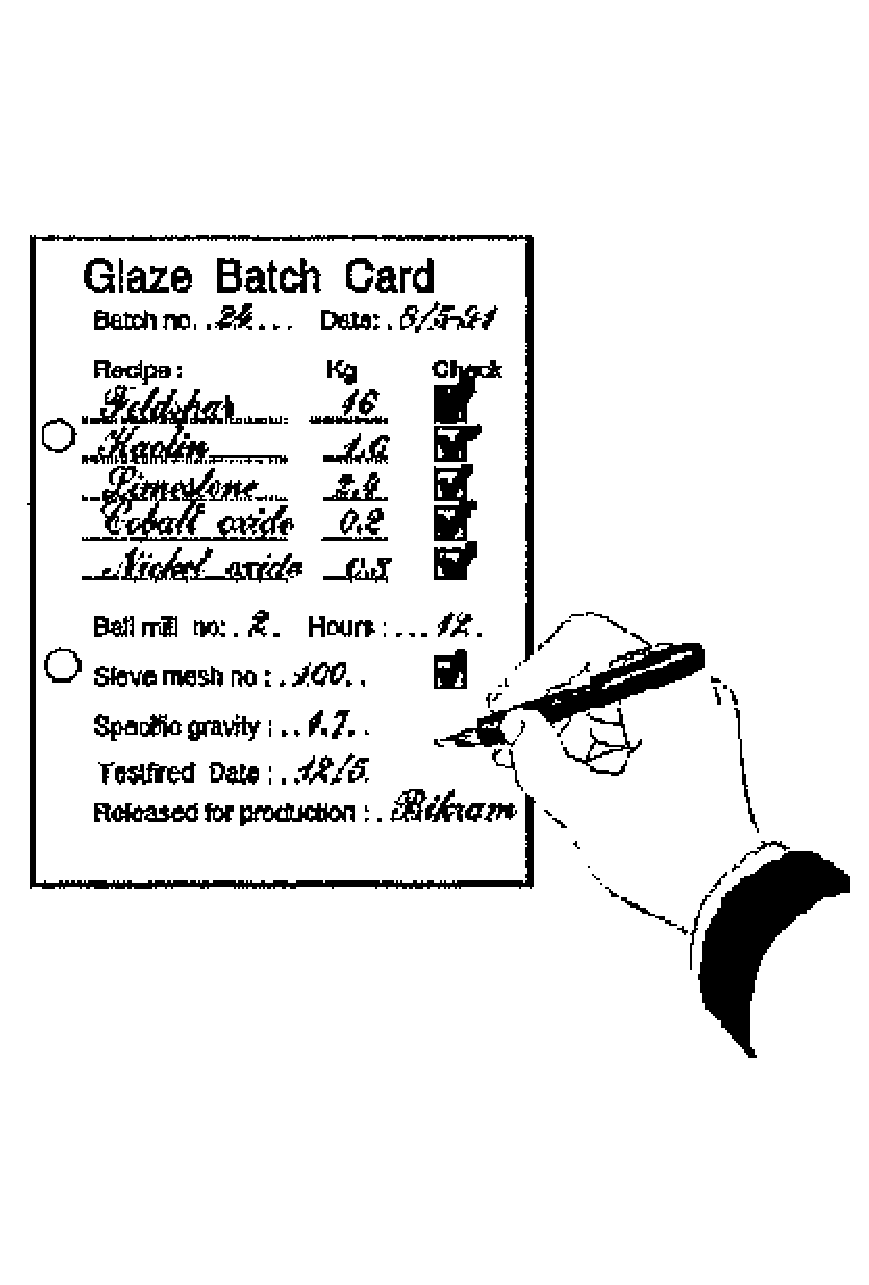
\includegraphics[width=0.8\linewidth]{img/batchcard.eps}
  \caption{Example of a glaze batch card used for qualitz control.}
  \label{fig:batchcard}
\end{figure}
%-------------------------------------------------------------------------------
\subsection{Batch Cards}
\label{sec:batchcard}
For best results, a batch card system should be used. These are simply cards 
that have the glaze recipe written on them. As each ingredient is weighed, it 
is checked off on the list. When all materials are weighed, the batch card is 
given a number (usually the date). The same number is written on the glaze 
container. This makes it easier to find out the problem when the glaze does not 
work correctly.
%------------------------------------------------------------------------------
\subsection{Water}
The ingredients are then added to a container which already has the approximate 
amount of water in it. 

\textbf{CAUTION:} The water must always be clean. After mixing, the water is 
adjusted. It is always best to start with less water than required. If the 
glaze is too fluid, it is difficult to remove excess water.
%------------------------------------------------------------------------------
\subsection{Containers}
Glazes are normally sieved through a 100-mesh screen. The glaze should be 
poured through without forcing it. Never use your hand to force glaze through a 
sieve, as this will quickly break down the wire mesh. A brush should be used 
instead.
%------------------------------------------------------------------------------
\section{Sieving}
Glazes are normally sieved through a 100-mesh screen. The glaze should be 
poured through without forcing it. Never use your hand to force glaze through a 
sieve, as this will quickly break down the wire mesh. A brush should be used 
instead.
%------------------------------------------------------------------------------
\section{Suspending and Binding Agents}
Because glazes are mixtures and not solutions, they tend to settle at the 
bottom of the container. Normally, the clay content of the glaze will be 
sufficient to keep them in suspension during application. However, some glazes 
tend to settle as a cement-like layer on the bottom and are difficult to stir. 
These glazes require the addition of a suspending agent.
%------------------------------------------------------------------------------
\subsection{Suspending Agent}
The most common suspending agent is bentonite, in 1-2\% additions. This will 
normally not be enough to affect the glaze when fired. Dry bentonite cannot be 
added to wet glaze, as it will just form lumps and be impossible to mix in 
thoroughly. Instead it should either be mixed separately with water into a thin 
slip and then added to the glaze or it should be added to the dry glaze and 
mixed in well before adding water.
%------------------------------------------------------------------------------
\subsection{Binder}
Another common problem is that some glazes tend to be powdery, and come off 
when loading the kiln. For this problem a binder is added.

Bentonite also works as a binder and is the simplest to use. Another common 
binder is CMC gum (carboxymethyl cellulose), which is available in either 
liquid or powder form. The liquid can be used directly, about 1\%. The powder 
needs to be dissolved in water (1:10) overnight and then is added to the glaze 
as liquid.

Organic binders such as gum arable, wheat flour, sugar or starch (0.1--0.5\% of 
dry glaze) are sometimes used. These have the disadvantage of fermenting. They 
should be used immediately after mixing, or if stored a few drops of chlorine 
bleach or formaldehyde can be added as a preservative.

Addition of 1\% raw borax produces a hard surface that does not powder when 
painted on.
%------------------------------------------------------------------------------
\subsection{Flocculation}
Addition of a flocculation agent will make the glaze more creamy. The pottery 
will absorb the water more easily so glaze is picked up faster.

This works better in combination with clay or bentonite. Common flocculants 
are: Epsom salts (magnesium sulfate), calcium chloride, calcium nitrate and 
borax. They are prepared by adding 100 g flocculant to 200 ml hot water and the 
solution is added to the glaze one tablespoonful at a time (up to 1\% of dry 
glaze weight). Plaster of parts (already set) can also be used.

Flocculation is also used for nonporous ware often in combination with a 
binder. The creamy glaze forms a thick loose layer that stays on the nonporous 
surface.
%------------------------------------------------------------------------------
\subsection{Deflocculation}
When the glaze is deflocculated it becomes more fluid with the same amount of 
water. This is sometimes used for glazing nonporous ware that cannot absorb 
water. Sodium silicate and soda ash are the most common deflocculants and they 
are prepared in the same way as flocculants.

\textbf{CAUTION:} Binders, deflocculants or flocculants should only be added 
after the glaze is ball-milled.
%------------------------------------------------------------------------------
\section{Density and Specific Gravity}
Most potters judge the consistency of their glaze by experience and feel, or by 
test application to a few pieces of biscuit to see if the thickness is correct. 
The standard test is to check thickness with a fingernail, which is a very 
accurate test for an experienced glazer. Then adjust the water as necessary.

A more accurate method is to measure the specific gravity of the glaze with a 
hydrometer, such as is commonly used to judge the amount of water that has been 
mixed with milk. When reading the depth the hydrometer sinks, take care that it 
is really showing the correct density. If the glaze is thick you have to 
vibrate the bucket repeatedly to make sure the hydrometer sinks in.

Specific gravity (s.g.) is a measure of the density of a liquid compared to 
water, which has a standard specific gravity of 1. Glazes will always be 
heavier than water. The specific gravity is found by weighing a specific 
volume, say 1000 ml (milliliters). If this weighs 1500 g the s.g. is 1.5. 
Weighing is more accurate than using a hydrometer.

After you find out the correct amount of water by trial and error, the specific 
gravity can be measured and future batches of the same glaze made to the same 
specific gravity.

\textbf{CAUTION:} This is not always a reliable method because the water 
absorption of your biscuit will vary with its firing temperature. The water 
will still need to be adjusted by trial and error. Trial application and 
testing with a fingernail still constitute the most reliable method.
%-------------------------------------------------------------------------------
\begin{figure}[htbp!]
  \centering
  \includegraphics[width=0.8\linewidth]{img/Hydrometer.eps}
  \caption{Hydrometer made from a glass test tube..}
  \label{fig:Hydrometer}
\end{figure}
%-------------------------------------------------------------------------------
\section{Old Glazes, and Problems}
If you keep wet glazes around for a long time, they will usually have problems 
with settling or drying up. These glazes can still be used but it will be 
necessary to adjust the water and to resieve them. If the glaze is extremely 
thick, it is sometimes best to dry it out completely, crush it and remix it.

Before using a glaze that has set in the bucket for a few days, it should 
always be sieved through 60 or 100 mesh.

Too much water in the glaze is also a problem. The glaze can be allowed to 
settle and excess water carefully taken off the top. 

\textbf{CAUTION:} With soluble glazes, this can remove some of the ingredients 
and result in a glaze that no longer works correctly. In this case, the water 
should be allowed to evaporate until the thickness is correct.

Glazes made with raw borax, or incomplete borax frits, will often grow 
crystals. These cannot be sieved. The glaze should be dried out, the crystals 
crushed and remixed.

Some glazes will develop mold and begin to smell. Although they can still be 
used, it is probably better to just throw them out.
%-------------------------------------------------------------------------------
\section{Test Your Glazes}
The wise potter will never glaze a kilnload with untested glaze. Enough glaze 
should be kept on hand, so that each new batch can be test-fired in the regular 
glaze firing before it is used for application.
%-------------------------------------------------------------------------------
\section{Commercial Production of Glazes}
Glazes that are sold commercially are usually in dry powder form. They are made 
as standard glazes by ball milling, then are dried and packaged.

These glazes are simply mixed with the correct amount of water and sieved 
before using.
%-------------------------------------------------------------------------------
\chapter{Glaze Application}
Glaze application is a skill that takes some time to learn. In order to get 
consistent results, it needs to be done carefully and the same way every time. 
Thin and thick application will give different results, and careless 
application is always ruinous.

Glazing should be done just before loading the kiln, as glazed pieces that lie 
around gather dust and get damaged. Some glazes tend to crawl if fired right 
after glazing. If you have such problems, allow the glazed ware time to dry 
completely before firing.
%-------------------------------------------------------------------------------
\section{Work Place, Cleaning Area}
Before glazing, you should have a neat and clean area to work in. Dust 
thoroughly and remove small children. The biscuit to be glazed should be 
organized in one place, with all like items grouped together (cups, bowls, 
vases etc.). Ware boards are cleaned and arranged, ready to take the glazed 
ware to the kiln. The glaze should be sieved and checked just before starting 
the application. Clean water and sponges should be available.

Large items are usually glazed first, as they require a full bucket for even 
application.

Correct application depends on many different factors:
%-------------------------------------------------------------------------------
\begin{itemize}
\item Density of the glaze
\item Viscosity of the glaze
\item Particle size (depending on grinding time)
\item Expertise of the worker
\item Porosity of the biscuit
\item Thickness of the piece
\item Dipping time.
\end{itemize}
%-------------------------------------------------------------------------------
Although some of these factors can be controlled accurately in large 
industries, the small producer will have to depend on experience. Mistakes will 
be made at first, and it is important to be able to understand what went wrong, 
so it can be corrected.
%-------------------------------------------------------------------------------
\section{Application Methods}
The particular method of applying glaze depends on the type of ware -small, 
big, sculpture, tiles, open forms, closed forms etc.

Generally the inside of an object is glazed before the outside, to prevent 
handling defects.

Loading systems need to be considered carefully. Most pots are loaded on 
shelves directly, so the feet must be left unglazed. If foot rings are to be 
glazed, then each piece must be individually set on special kiln furniture in 
the kiln.
%-------------------------------------------------------------------------------
\subsection{Painting}
Glaze is sometimes applied with a brush. This is not recommended because it 
takes a great deal of skill to obtain an even coat, as well as a lot of time. 
Painting is used on sculptural objects that cannot be dipped or sprayed. Three 
to four coats are brushed on, letting each coat dry before applying the next. 
In order to see each coat, sometimes organic color dye (food coloring) is added.
%-------------------------------------------------------------------------------
\subsection{Dipping and Pouring}
Dipping and pouring constitute the most common method.

The glaze needs to be stirred frequently during application time.
%-------------------------------------------------------------------------------
\subsubsection{Cups and Bowls}
Cups can be glazed inside and out in one movement (after some practice). Hold 
the cup by the foot and dip it at a slant to let glaze inside, while the 
outside is also coated with glaze. Then quickly pull up and push down. This 
results in a ``fountain'' of glaze that covers the entire inside.
%-------------------------------------------------------------------------------
\begin{figure}[htbp!]
  \centering
  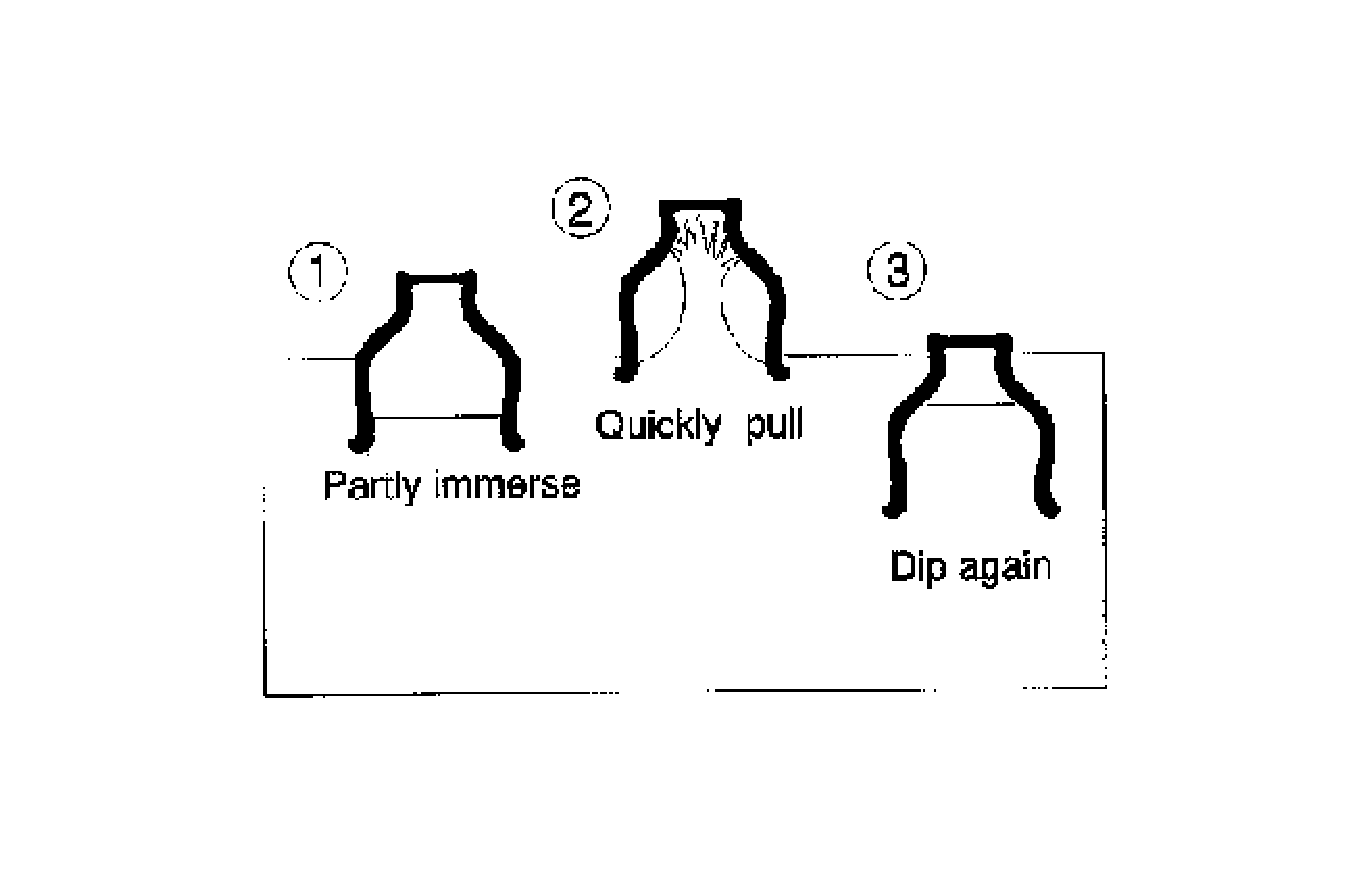
\includegraphics[width=0.7\linewidth]{img/glazingcup.eps}
  \caption{Three steps of glazing the inside and outside of a cup in one dip.}
  \label{fig:glazingcup}
\end{figure}
%-------------------------------------------------------------------------------
\subsubsection{Tiles}
To dip tiles, hold them by the edges and dip them in the glaze while moving 
sideways. This also requires practice!
%-------------------------------------------------------------------------------
\begin{figure}[htbp!]
  \centering
  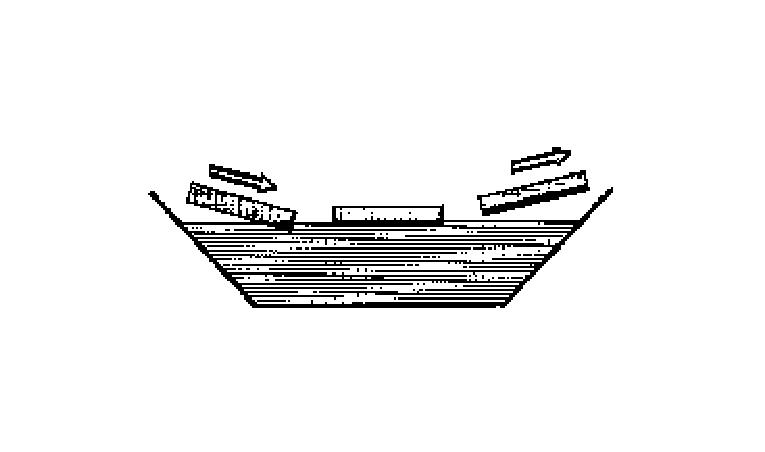
\includegraphics[width=0.7\linewidth]{img/glazingtile.eps}
  \caption{Dipping tiles in glaze.}
  \label{fig:glazingtile}
\end{figure}
%-------------------------------------------------------------------------------
\subsubsection{Double Dipping}
Applying a second coat of the same or a different glaze over the first is known 
as double dipping. This often happens inadvertently. When glazing the inside, 
sometimes there will be runs of glaze on the outside. These should be sponged 
clean before doing the outside. Larger items are often partly dipped to cover 
the top, then turned over and dipped again to coat the bottom. This usually 
results in a line of double glaze, which will look different. If the 
overlapping area is chosen carefully, it can become a part of the design. 
Otherwise, it will look like a mistake.

For decorative effects, a pot is sometimes dipped partly in one glaze and then 
again in a different glaze. This results in a third color where the two overlap.
%-------------------------------------------------------------------------------
\subsubsection{Waterfall Glazing}
In the commercial glazing of tiles, the ``waterfall'' system is used. This 
consists of a conveyor belt, which carries the tiles under a thin waterfall of 
glaze that pours over them. The thickness of application is controlled by the 
speed of the conveyor belt and the amount of glaze flow. Excess glaze runs into 
a tank, which is again pumped up to the waterfall. These machines are often 
equipped with automatic cleaners that take excess glaze off the sides of the 
tiles.
%-------------------------------------------------------------------------------
\begin{figure}[htbp!]
  \centering
  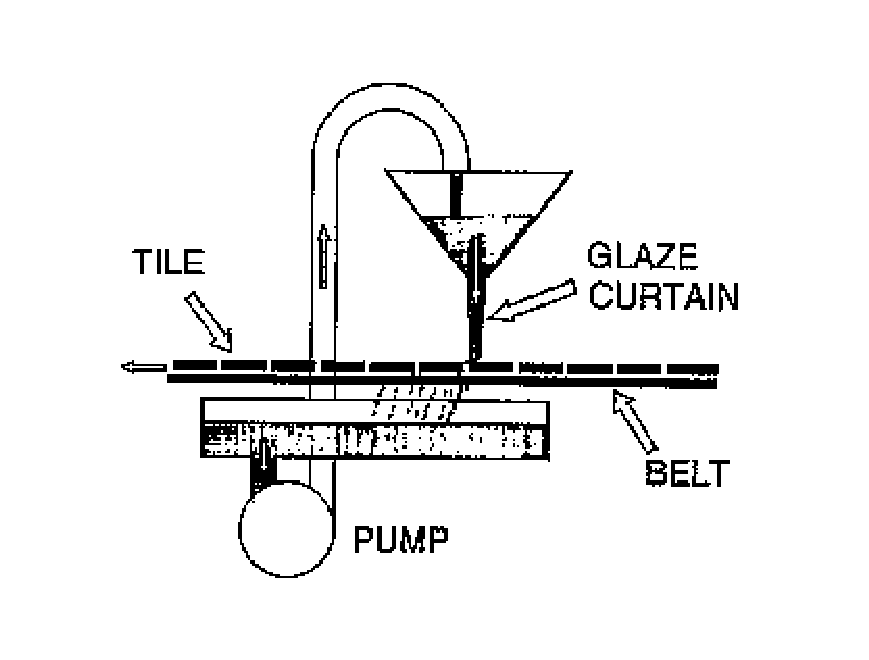
\includegraphics[width=0.7\linewidth]{img/glazingwaterfall.eps}
  \caption{Waterfall glazing of tiles. The tiles run through a curtain of glaze 
  which is continuously recycled with the help of a pump.}
  \label{fig:glazingwaterfall}
\end{figure}
%-------------------------------------------------------------------------------
\subsection{Spraying}
Spraying is used for items that cannot easily be dipped or poured. It requires 
an air compressor and a spray gun, as well as a spray booth equipped with an 
exhaust fan. This is not recommended for the small producer, unless it is 
required for frequent use or for special decorative effects. Ordinary spray 
guns for paint can be used, but they wear out quickly because glaze is 
abrasive. Special spray guns for glaze are equipped with silicon carbide spray 
heads.

Spraying has the disadvantage of wasting a lot of glaze that goes into the air. 
This is dangerous to inhale, and a spray booth should be provided with an 
exhaust fan to the outside, as well as having a filter to catch excess glaze. 
If a great deal of spraying is done, the excess glaze can be collected from the 
filter and the inside of the booth and reused.

As usual, the inside of the item is glazed first (usually by pouring), and the 
spraying is done in several even, systematic coats. Each one must be applied 
before the first one dries, or the glaze may lift off the pot. Each coat should 
be lightly applied, so that it looks a bit powdery.

It is difficult to judge the correct thickness of glaze and to get it even all 
over, especially in difficult areas like under handles. In time the glazer will 
learn to measure the thickness by feeling it with a fingernail.
%-------------------------------------------------------------------------------
\subsubsection{Airbrush}
An airbrush is a very small spray gun that can be adjusted from a pencil-thin 
spray to a wide pattern. These are not used for glaze application, but are 
often used for decorative effects-with underglazes and overglazes.
%-------------------------------------------------------------------------------
\subsubsection{Care of the Spray Gun}
Spray guns are very sensitive. They tend to get clogged, so make sure that your 
glaze is sieved before putting it in the gun. Clean the spray gun immediately 
after use by rinsing it out and spraying clean water through it until there is 
no sign of glaze. Glaze left in the spray gun will corrode it and make it 
unusable.
%-------------------------------------------------------------------------------
\subsubsection{Glaze Fountain}
For glazing the inside of large items a glaze fountain as shown in 
figure~\ref{fig:glazingcup} is helpful. The pot is placed over a nozzle from 
which an electric pump provides a powerful upward shower of glaze when 
activated with a switch on the floor.
%-------------------------------------------------------------------------------
\section{Density, Binders, Glaze Thickness}
As described above, it is important to have the correct a nouns of water in 
your glaze. The glaze should always be checked and corrected by test dipping 
some biscuit before starting and then relying on your experience to judge if 
the thickness is correct. Checking specific gravity with a hydrometer or by 
weighing is a good practice but should not be relied on.

It is best not to use binders unless you have no choice. CMC gum is the most 
satisfactory.
%-------------------------------------------------------------------------------
\subsubsection{Non-porous Biscuit}
As previously mentioned, differences in biscuit firing temperature cause 
differences in porosity and can cause problems in glaze application. Overfired 
biscuit is especially difficult to glaze, as it will not absorb water. In the 
making of whiteware, the biscuit temperature is usually higher than the glaze 
temperature. This results in a semivitrified body that has special glaze 
application problems. If it is necessary to reglaze pots that have firing 
defects, they also require special handling.

If you only have a few pieces, they can be heated until almost too hot to 
handle and then dipped, poured or sprayed (spraying is most satisfactory). The 
heat will make excess water evaporate.

If glazing vitrified ware is part of your standard production, then it is best 
to flocculate your glaze. This is the opposite of deflocculation (as used with 
casting slip) and results in a thick, pudding-like glaze with the normal water 
content.
%-------------------------------------------------------------------------------
\section{Waxing}
In order to keep glaze from being applied to the foot of your pots, it is often 
more efficient to wax the bottoms as compared to sponging them clean. The 
coating of wax prevents glaze from sticking. There are two common waxing 
methods:
%-------------------------------------------------------------------------------
\subsubsection{Hot Wax}
Paraffin wax is kept melted in a shallow metal pan over an electric heater or 
a smoldering charcoal fire (an open fire should not be used as the paraffin 
may start to burn). It should be hot, but not so hot that it starts to smoke. 
Before applying the glaze, the foot rings are dipped in the paraffin.
%-------------------------------------------------------------------------------
\subsubsection{Liquid Wax Resist}
It is much easier to use liquid wax resist, which is a wax emulsion in a 
water base. It can be thinned with water but after drying cannot be 
dissolved. This is commercially available in some countries specifically for 
glaze application. It is also possible to use liquid floor wax.

Liquid wax resist is also used for decoration.
%-------------------------------------------------------------------------------
\section{Single-Fire Glazing}
Single-fire glazing is sometimes called ``raw glazing'', but this term is 
confusing as ``raw glaze'' also is used for unfritted lead or borax glazes. 
Glaze is applied directly to bone-dry or leather-hard ware and fired once up to 
the glaze temperature. Not all glazes and bodies are suitable for single 
firing, and each combination needs to be tested.

Glazes that work on biscuit ware will often also work on bone-dry clay with a 
small addition of a plastic clay or bentonite. Glazes for leather-hard glazing 
will need more clay so the glaze layer will shrink along with the clay during 
drying. The leather-hard method is less practical, since each batch of 
leather-hard pots must be glazed immediately, causing problems in the work flow.

The advantage of single firing is that it avoids the fuel and extra handling 
needed for biscuit firing. The main problem with single firing is crawling 
caused by different shrinkage rates of clay and glaze in the early stages of 
the firing. Single-fire glazes usually have a high percentage of clay.

Delicate ware cannot usually be single-fired successfully, as it tends to be 
damaged by the water.

Single-fire glazing needs to be done quickly and carefully, without letting 
glaze stand inside the pot for a long time. Dipping and pouring can be used, 
and spraying is also effective.

Firing needs to be done more slowly than usual, so that pots do not explode. 
The early stages of firing should be done as with biscuit firing.

Single firing is used most often in large tile industries, where it saves fuel.
%-------------------------------------------------------------------------------
\section{Handling, Drying Before Firing}
Good glaze application requires careful handling. Many pots are spoiled by 
fingerprints or glaze that is knocked off during handling. Pots should be 
allowed to dry before loading in the kiln.

The kiln loader should be responsible for checking each pot as he places it in 
the kiln. This means inspecting the foot to see if it is clean and rejecting 
pots with damaged or thick glaze. The loader should constantly clean his hands 
of glaze dust especially when loading ware with different colored glazes. 
Otherwise colored fingerprints will mark the pots.
%-------------------------------------------------------------------------------
\section{Salt Glazing}
In salt glazing, no glaze is actually applied to the pot before firing. The 
ware is single-fired up to the maturing point of the clay and rock salt is then 
introduced directly into the firebox. The salt breaks down into sodium and 
chlorine gas. The sodium combines with silica on the surface of the pot to make 
a durable glaze and the chlorine goes up the chimney, combining with water in 
the air to form hydrochloric acid. This is an irritant, as well as causing 
damage to vegetation and metal structures in the immediate vicinity. Another 
problem is that the salt erodes the firebricks in the kiln rather fast.

Salt glazing normally is done on stoneware at temperatures above 1100\degree C. 
Salt is often mixed with borax to lower the melting point (see also 
section~\ref{sec:meltingpointsec}).
%-------------------------------------------------------------------------------
\chapter{Decoration}
Decoration is a very big field, which deserves a separate book to cover it in 
detail. Here we will only discuss some of the main techniques for using glazes 
and engobes.
%-------------------------------------------------------------------------------
\section{Decoration and Design}
The main reason for decorating pots is for pure enjoyment. As pottery is 
something that is used intimately every day, it should be attractive and 
interesting, besides being simply functional. Decorated pottery also has a 
better market value and often more than pays for the extra time taken.
Good decoration is always related to the design of the pot. It should be used 
to emphasize and enhance the shape of the pot, rather than being applied 
randomly.

There are several approaches to decoration:
%-------------------------------------------------------------------------------
\subsubsection{Banding}
Plain or decorative bands of color are painted around the pot, usually by 
spinning the pot on a banding wheel and applying color with a brush. The bands 
are placed where they emphasize changes in the curve of the pot, for example, 
at the rim, the belly, the shoulder.
%-------------------------------------------------------------------------------
\subsubsection{Area Decoration}
Decoration is placed inside a defined area, such as a circle. Again this should 
be done to emphasize the natural curves of the pot.
%-------------------------------------------------------------------------------
\subsubsection{Overall Patterns}
These are patterns that are repeated around the pot, often expanding and 
contracting as the pot does.
%-------------------------------------------------------------------------------
\subsubsection{Contrasting Shapes}
These are strongly shaped areas of pattern or color that contrast with the 
shape of the pot.
%-------------------------------------------------------------------------------
\subsection{Motifs, Styles, Local Inputs}
There are as many motifs and styles of decoration as there are cultures in the 
world. In traditional cultures, motifs are selected from mythology and familiar 
designs. Nowadays, with the mixing of cultures around the world, pots are often 
designed for what can be marketed for export, and design tends to be based on 
fashion rather than tradition.

The potter selling to tourists will generally choose traditional motifs, since 
tourists are interested in the culture of the area.
%-------------------------------------------------------------------------------
\section{Glaze Decoration}
Glaze decoration is done with the glaze itself or with colorants under the 
glaze or on top of the glaze.
%-------------------------------------------------------------------------------
\subsection{Underglaze}
Underglaze decoration is decoration that is applied under the glaze. It is 
affected by the transparency and fluidity of the glaze.

Underglazing is usually done under a transparent glaze in order to show it 
clearly. However, beautiful effects can be obtained under opaque or semiopaque 
glazes.

A variety of pigments and oxides may be used.
%-------------------------------------------------------------------------------
\subsubsection{Metallic Oxides}
The more fusible metallic oxides can be used directly as underglaze pigments, 
mixed thinly with water. The satisfactory ones are red iron oxide, cobalt 
carbonate, manganese dioxide and copper carbonate. Designs made with oxides 
alone will often run with the glaze. Refractory oxides, such as chrome oxide 
and rutile, can cause crawling.
%-------------------------------------------------------------------------------
\subsubsection{Oxides Mixed With Glaze}
Metallic oxides can be mixed about 50/50 with glaze, which will prevent the 
problem of crawling. However, the decoration will usually flow with the glaze 
and should be designed with this in mind.
%-------------------------------------------------------------------------------
\subsubsection{Underglaze Pigments}
These are pigments that are specially prepared by fritting metallic oxides in a 
base glaze that fires hard but is not fluid. Rather than preparing them 
yourself, it is usually better to purchase commercial underglazes from a 
supplier. These are supplied for venous firing temperatures and firing 
conditions in a wide range of colors. Not all colors can be used under all 
conditions, and suppliers can usually tell you which are suitable for oxidation 
and reduction and what type of base glaze will develop the best colors.
%-------------------------------------------------------------------------------
\subsection{On-Glaze}
On-glaze decoration is applied on top of the unfired glaze. It may be done with 
a contrasting color of glaze or with metallic oxides or glaze pigments.

Application is done by brushing or spraying. Even more than underglaze, 
on-glaze decoration will tend to flow with the glaze. If distinct patterns are 
desired, a stiff, viscous glaze will give the best results.
%-------------------------------------------------------------------------------
\subsubsection{Double Glazing}
Glazes high in surface tension (see section~\ref{sec:surfacetension}) tend to 
form into small islands on melting. This may cause crawling, but it can also be 
used as a decorative effect by applying two different glazes on top of each 
other. The glazes must have different degrees of surface tension. This is 
achieved by adding clay or talc to one of the glazes. The colors should be 
contrasting. The best results are obtained with a light-colored glaze at the 
bottom.
%-------------------------------------------------------------------------------
\begin{figure}[htbp!]
  \centering
  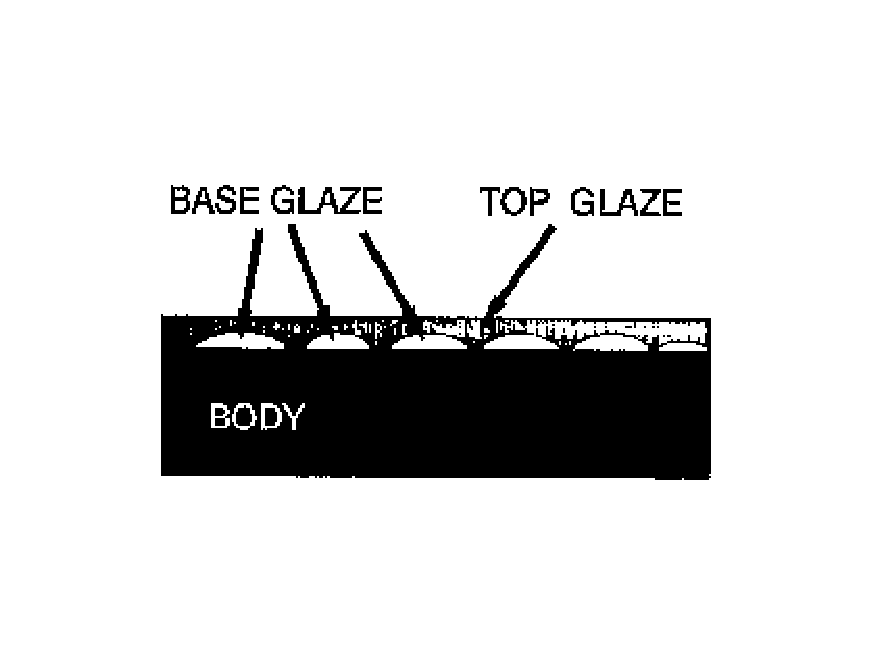
\includegraphics[width=0.7\linewidth]{img/doubleglazinghigh.eps}
  \caption{Double glazing with the high-surface-tension glaze on top. This 
  draws itself into islands leaving the bottom glaze in irregular patterns.}
  \label{fig:doubleglazinghigh}
\end{figure}
%-------------------------------------------------------------------------------
\begin{figure}[htbp!]
  \centering
  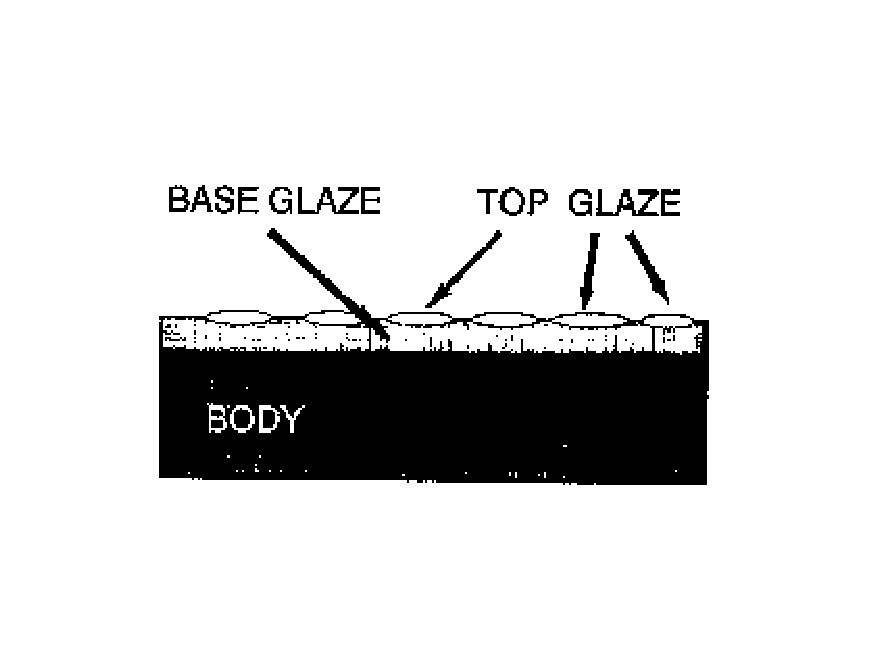
\includegraphics[width=0.7\linewidth]{img/doubleglazinglow.eps}
  \caption{Double glazing with the low-surface-tension glaze on top. This 
  produces a different effect.}
  \label{fig:doubleglazinglow}
\end{figure}
%-------------------------------------------------------------------------------
\subsection{Overglaze}
Overglaze decoration is often called ``china painting''. The pot is glaze-fired 
as usual and then is decorated with special low-temperature enamels that fire 
at around 700\degree C. The enamels are prepared from color pigments and 
low-temperature frits and are best purchased from commercial suppliers. They 
are available in every color and have the advantage of firing to true colors, 
making them suitable for elaborate painting effects. They also stay where they 
are applied, as there is no chance of the glaze running at this low temperature.

Overglaze is available as powder, which must be mixed with a medium. This is 
best done by grinding the pigment and medium on a glass plate with a thin 
palette knife.

Sometimes plain water is used: this works well when filling areas with solid 
colors. It helps to add some water-soluble glue (white glue) to provide dry 
strength.

For more elaborate painting, pigment is mixed with special oils. The best is 
oil of lavender, which is thickened as desired with a thicker oil. The 
consistency is controlled very much like with oil paint.

Some suppliers have ready-mixed overglaze, which comes in tubes. This can be 
used directly, without grinding.

Special metallic or iridescent overglazes are known as ``luster''. These are 
available commercially as liquid gold, platinum and a variety of mother of 
pearl colors. They also are fired at 700\degree C. 

\textbf{Note:} Lusters take on the same surface as the glaze, i.e. a matt glaze 
will produce a matt luster and a shiny glaze will give a mirror-like effect.

Overglazes are applied by brushing or by spraying.
%-------------------------------------------------------------------------------
\subsubsection{Overglaze Transfers or Decals}
Most commercially sold decorated dinnerware is decorated with decals (sometimes 
called transfers), which are made from overglaze that is silkscreen-printed 
onto decal paper. These are available from suppliers in a range of standard 
designs and can also be custom-made (in large quantities). They are applied to 
already glaze-fired ware.

The decal is soaked in water until the design can easily be slid off the paper. 
The wet paper is placed in the correct location and is carefully slid from 
under the design, leaving the design adhered to the pot. The design is 
carefully smoothed, dried and fired like standard overglaze.
%-------------------------------------------------------------------------------
\subsection{Reglazing, Multiple Glazing}
Reglazing means applying glaze and firing an article that already has been 
fired once. It is sometimes necessary when glazes do not work correctly the 
first time -they may be too thin, underfired or not the right color.

Multiple glazing is the process of glazing and firing an article two or more 
times in order to get special glaze effects that cannot be achieved in one 
firing. It often involves first glaze firing the pot at a high temperature and 
then glaze firing with lower temperature glazes, in order to get special colors 
or textures. For example, a pot may be fired to cone 10, then be refired with 
cone 06 glazes to get bright colors. It may be fired several times at cone 010 
for overglazes and lusters.

Reglazing or multiple glazing makes an article more expensive, but it can also 
be sold at a much higher price.
%-------------------------------------------------------------------------------
\subsubsection{Reglazing Hints}

Because already fired ware is no longer porous, it is difficult to apply enough 
glaze. It helps to first heat the article (as hot as you can hold in your 
hand), and spraying is the most effective way to apply more glaze.

For multiple glazing, glaze can be specially prepared by adding cellulose gum 
(CMC). This thickens the glaze and gives it better handling strength.
%-------------------------------------------------------------------------------
\section{Engobe Decoration}
Engobe is a specialized type of clay slip that is used for decoration under the 
glaze. The engobe shows through a transparent or semitransparent glaze and can 
have the range of color that is possible in glaze.
%-------------------------------------------------------------------------------
\subsection{Advantages and Disadvantages, as Compared to Glaze Decoration}
Engobes stay where they are applied and do not run with the glaze. This makes 
it possible to do designs with sharp edges or a lot of detail.

Engobes are often used on dark clay bodies in order to provide a bright, white 
background for glazes.
%-------------------------------------------------------------------------------
\subsection{Engobe Making, Adjusting to Body}
Engobe is generally prepared as a white base and then colored with appropriate 
coloring oxides. If you are already using a white clay body, this becomes an 
engobe simply by thinning it with water. A dark body will require a white 
engobe formula that fits it correctly.

The main problem with engobe is getting a good fit between engobe and clay 
body. It must have about the same amount of shrinkage as the body or it will 
tend to flake off or crack. The engobe should also mature at the same 
temperature as the clay body in order to provide a strong clay-glaze interface. 

Usually engobes designed for plastic clay will not fit on bone dry or biscuit 
clay and vice versa.

Some typical engobe recipes are shown in table~\ref{tab:engoberecipes}

Engobes can be applied at three different stages.
%-------------------------------------------------------------------------------
\subsubsection{Leatherhard}
This is the best stage for applying engobes, as it permits the widest range of 
decorating techniques (brushing, incising, inlaying, stencil etc. -see below). 
The engobe must have enough clay in it to shrink at the same rate as the body.
%-------------------------------------------------------------------------------
\subsubsection{Bone-Dry}
Engobes for bone-dry application need to have less shrinkage, so that they 
adhere to the body.
%-------------------------------------------------------------------------------
\subsubsection{Biscuit}
Engobes for biscuit application are more like underfired glazes.
%-------------------------------------------------------------------------------
\begin{landscape}
\begin{center}
  \renewcommand{\arraystretch}{1.5}
  \begin{table}\centering
    \begin{tabular}{|c||c|c|c||c|c|c||c|c|c|}\hline
 \textbf{Temperature Range}
&\multicolumn{3}{c}{\textbf{Cone 08--1}}\vline
&\multicolumn{3}{c}{\textbf{Cone 1--6}}\vline
&\multicolumn{3}{c}{\textbf{Cone 6--11}}\vline\\\hline\hline
      
%-------------------------------------------------------------------------------
\textbf{Body Condition}
&\textbf{Damp}&\textbf{Dry}&\textbf{Biscuit}
&\textbf{Damp}&\textbf{Dry}&\textbf{Biscuit}
&\textbf{Damp}&\textbf{Dry}&\textbf{Biscuit}\\\hline\hline
%------------------------------------------------------------------------------
Kaolin&25&15&5&25&15&5&25&15&5\\\hline
%------------------------------------------------------------------------------
Ball Clay&25&15&15&25&15&15&25&15&15\\\hline
%------------------------------------------------------------------------------
Calcined Kaolin&-&20&20&-&20&20&-&20&20\\\hline
%------------------------------------------------------------------------------
Leadless Frit&15&15&15&-&-&5&-&-&5\\\hline
%------------------------------------------------------------------------------
Nepheline Syenite&-&-&-&15&15&20&-&-&5\\\hline
%------------------------------------------------------------------------------
Feldspar&-&-&-&-&-&-&20&20&20\\\hline
%------------------------------------------------------------------------------
Talc&5&5&15&5&5&5&-&-&-\\\hline
%------------------------------------------------------------------------------\\
Quartz&20&20&20&20&20&20&20&20&20\\\hline
%------------------------------------------------------------------------------
Opacifier (Zircon)&5&5&5&5&5&5&5&5&5\\\hline
%------------------------------------------------------------------------------
Borax&5&5&5&5&5&5&5&5&5\\\hline
%------------------------------------------------------------------------------
\end{tabular}
\caption{Typical Engobe Recipes per Daniel Rhodes.}
\label{tab:engoberecipes}
\end{table}
\end{center}
\end{landscape}
%-------------------------------------------------------------------------------
\subsubsection{Engobe Composition}
Engobe is made up of a mixture of plastic and nonplastic ingredients. Recipes 
for engobes look like those for glazes with a high percentage of refractory 
ingredients.

For white engobes, the plastic ingredients are china clay and ball clay. The 
amount of ball clay can be adjusted to get correct shrinkage.

The nonplastic ingredients are feldspar and quartz, and for low-temperature 
engobes frit is sometimes added to lower the vitrification point.

Small amounts of borax are often added to give better dry strength and to fuse 
the other ingredients together.

Engobes are often deflocculated like a casting slip, and in fact you can often 
use a casting slip which fires at the same temperature as your clay body.
%-------------------------------------------------------------------------------
\subsection{Color Oxide Additions to Engobe}
Coloring oxides are added to engobes as a percentage, as with glazes. However, 
since the color is diluted by the glaze over it, larger amounts are required. 
You should also remember that the oxide reactions will depend on the type of 
glaze being applied and on whether oxidation or reduction firing is used. 

As with glaze colorants, the most interesting colors are usually obtained by 
mixing combinations of oxides.

Table~\ref{tab:engobeoxides} shows the typical oxides used in engobes, and 
their resulting colors.
%-------------------------------------------------------------------------------
\begin{center}
  \begin{table}\centering
    \renewcommand{\arraystretch}{1.5}
\begin{tabular}{|c|c|c|}\hline
 \textbf{Oxide}&\textbf{Percent}&\textbf{Color}\\\hline\hline
&1--5\%&Light green to light brown\\\cline{2-3}
Red Iron Oxide&5--10\%&brown\\\cline{2-3}
&10--15\%&dark brown to black\\\hline
Copper oxide or carbonate&1--5\%&Green or blue. (Red in reduction)\\\hline
Cobalt oxide or carbonate&1--5\%&Light to dark blue\\\hline
Chrome oxide&1--5\%&Green\\\hline
Manganese oxide&1--10\%&Purple-brown\\\hline
Nickel oxide&1--5\%&Grey or green-grey\\\hline
Titanium dioxide (Rutile)&1--10\%&Tan, or mottled colors\\\hline
Commercial stains&1--50\%&The color of the stain\\\hline
\end{tabular}
\caption{Typical oxide amounts in engobes, and the resulting colors.}
\label{tab:engobeoxides}
\end{table}
\end{center}
%-------------------------------------------------------------------------------
\subsection{Application Methods}
A wide variety of decoration techniques can be used with engobe. Leather-hard 
ware permits the largest variety of techniques and usually has fewer technical 
problems compared to application on bone-dry or biscuit ware. Work flow for 
leather-hard engobe decoration is:
%-------------------------------------------------------------------------------
\begin{enumerate}
  \item Apply the engobe
  \item Biscuit fire
  \item Apply the glaze
  \item Glaze fire
\end{enumerate}
%-------------------------------------------------------------------------------
\subsubsection{Dipping, Pouring}
This is done the same as with glazes. The engobe should be just thick enough to 
completely cover the clay. Too thick application will often crack, especially 
on rims. If applied leather-hard, pouring and dipping should be done quickly, 
so that the pot does not get too soft from absorbing water.
%-------------------------------------------------------------------------------
\subsubsection{Brushing}
Brushing is one of the most satisfactory methods, especially for making bands 
or areas of engobe. The technique requires some skill in order to get an even 
coating. The brush should be fully loaded with engobe and should spread it 
evenly.
%-------------------------------------------------------------------------------
\subsubsection{Spraying}
The engobe must be thin enough to flow through the spray gun. It should be 
applied in several even coats, taking care to keep a smooth surface and to 
cover all areas equally.
%-------------------------------------------------------------------------------
\subsubsection{Scratching or ``Sgraffito''}
To get fine lines, engobe is applied to an area and, after it sets, it is 
scratched with a sharp tool. This is called ``sgraffito'', which means 
``scratching''. The clay color shows as a line.
%-------------------------------------------------------------------------------
\subsubsection{Inlay}
Lines are scratched on the leather-hard pot and then filled with engobe. The 
excess engobe is removed with a metal scraper after it sets, or with sandpaper 
after the pot is bone-dry. This results in a smooth surface, with the engobe 
lines contrasting with the clay colon
%-------------------------------------------------------------------------------
\subsubsection{Stencil}
Paper or plastic stencils are placed on the leather-hard pot, and engobe is 
brushed or sprayed over them. Afterwards the stencil is removed leaving the 
design of the stencil.
%-------------------------------------------------------------------------------
\subsubsection{Trailing}
Usually called ``slip'' trailing, the engobe is applied by allowing it to flow 
from a device with a small opening, which produces raised line decoration. It 
is easiest to use a rubber bulb (such as an ear syringe available in 
pharmacies) or plastic containers used for soap or cosmetics. The opening can 
be made smaller by inserting small metal tubes.
%-------------------------------------------------------------------------------
\subsubsection{Hints}
Engobes will show most clearly under a fully transparent glaze. However, 
semitransparent or even opaque glazes can give beautiful effects, clouding the 
engobe colors.

Sophisticated decorators can take advantage of different glazes over the engobe 
to produce different colors. Complicated effects can result from applying 
different glazes to different areas of the decorated piece.
%-------------------------------------------------------------------------------
\subsection{Engobe Problems}
Often engobe will come off the pot. This almost always is caused by a different 
shrinkage rate of clay body and engobe and usually happens before firing. In 
many cases the engobe is applied too thick.
%-------------------------------------------------------------------------------
\subsubsection{Engobe Shrinks More Than The Clay Body}
In this case, the engobe will develop cracks and will flake off, with the 
flakes curling away from the ware. The solution is to reduce the amount of 
plastic clay or substitute raw clay with calcined clay. Deflocculating usually 
helps.
%-------------------------------------------------------------------------------
\subsubsection{Engobe Shrinks Less Thank The Clay Body}
In this case, the engobe will flake off, especially on rims and sharp edges, 
and the flakes will be flat. The solution is to add more plastic clay or to 
substitute calcined clay with raw clay.
%-------------------------------------------------------------------------------
\subsubsection{Flaking After Firing}
This is caused by differences in firing shrinkage between clay and engobe. 
Usually adding flux to the engobe will help.
%-------------------------------------------------------------------------------
\subsubsection{Spit-Outs}
Application of engobe to biscuit ware sometimes causes the engobe to lift off 
in small bubbles. This may only show up after glaze firing, but it arises 
during application. If the biscuit ware is very porous, it absorbs the water in 
the engobe so fast that air inside the body comes under pressure. When the air 
is released, it may blow out the engobe layer where the air escapes. The 
solution is to reduce the absorption by dipping the biscuit in water some time 
before engobe application.
%-------------------------------------------------------------------------------
\section{Terra Sigillata}
The technique of coating pottery with terra sigillata was used by Roman and 
Greek potters and is still used by traditional potters in India and Nepal. It 
produces a thin, opaque and low gloss finish to pottery.
%-------------------------------------------------------------------------------
\subsection{Preparing Terra Sigillata}
Terra sigillata is made from clay. For temperatures below 1100\degree C local 
sedimentary clays are more suitable. The finer the clay particles the better. 
Such clays normally contain iron and fire to a red colon It is more difficult 
to produce white-fring terra sigillata from ball clay or kaolin.

Table~\ref{tab:terrasig} shows a recipe for preparing terra sigillata.

The best result is obtained when ball milling the clay. Some clay can be 
prepared without ball milling. After ball milling the batch is transferred to a 
container and left for 24 hours. The coarse particles will settle and the upper 
2/3 of the batch is siphoned off. A bucket with a tap placed 1/3 up is useful 
for regular production of terra sigillata.

Colors can be made by adding color oxides or pigments. First the terra 
sigillata is dried and the color oxide is added in amounts similar to what is 
mentioned for engobes (by dry weight). Then water is added and the batch is 
again ball-milled for 4 hours. It is then ready for use.
%-------------------------------------------------------------------------------
\begin{table}\centering
  \renewcommand{\arraystretch}{1.5}
  \begin{tabular}{|c|c|c|}\hline
    &Clay&50\\\cline{2-3}
    By weight:&Water&100\\\cline{2-3}
    &Sodium metaphosphate&+5\%\\\hline
  \end{tabular}
  \caption{Recipe for terra sigillata.}
  \label{tab:terrasig}
\end{table}
%-------------------------------------------------------------------------------
\subsection{Application}
The terra sigillata should be adjusted to a density of 1.15 to 1.20 for 
application on leather-hard clay. For dry and biscuit ware more water is added 
to obtain a density of 1.05 to 1.10. The ware should be clean and dust-free 
before application.

Application can be done by dipping, brushing and spraying. After drying the 
gloss can be improved by polishing the surface with a cloth.
%-------------------------------------------------------------------------------
\subsection{Advantages}
The use of terra sigillata makes it possible to produce attractive decorations 
on low-fired pottery without using glazes. The coating gives a dense, glossy 
and impervious surface. A very beautiful glossy black can be produced by 
placing the terra sigillata items in a ridded pot filled with sawdust. This is 
fired in a normal firing either in a kiln or in a traditional pottery firing. 
The strong reduction will change the normal red color to black.

The use of terra sigillata coatings as an intermediate layer between body and 
glaze is reported to reduce crazing and bubbles in the glaze.
%-------------------------------------------------------------------------------
\chapter{Glaze Problems}
Anybody with even a little experience with glazes will realize that problems 
often arise. Knowing what to do about them requires a lot of experience, and 
even expert glazers often find it difficult to establish the source of a 
problem.
%-------------------------------------------------------------------------------
\section{Introduction to Glaze Problems}
It is one thing to develop a nice glaze but quite another to keep it working. 
One potter may want a glaze that crazes, whereas another wants his glaze to be 
craze-free. A glaze fault may not mean that the glaze is ugly, just that it 
reacts differently and does not look like the desired effect.

When a glaze suddenly starts to react differently from what we want, we call it 
a glaze fault. Solving the problem is seldom easy, and usually several factors 
are involved. The first thing to check is what changes have occurred since the 
glaze last worked without problems. 

The following things should be checked:
%-------------------------------------------------------------------------------
\begin{itemize}
\item Was the right recipe used and were the materials weighed out correctly? 
(Always use batch cards for glaze weighing).
\item Were the right raw materials used? Was there any chance of mistaking one 
material for another? Was the labeling of materials in stock correct?
\item Have new raw materials or a new frit batch been used since the last 
fault-free glaze batch was produced? If so, check if the new material is 
different from the original material in stock.
\item Has the body been changed in any way? For example: new preparation 
method, change of clay material, change of body recipe, higher or lower biscuit 
firing?
\item Was the preparation of the glaze done as usual? For example: same ball 
milling time, same screening, same specific gravity of glaze slip?
\item Was there any change in glaze application and were the products clean and 
dust-free before application?
\item Were there changes in the kiln setting? Was the glazed ware dry before 
firing started? Were there any changes in fuel, firing schedule, firing 
atmosphere (reducing/oxidizing) and was the correct top temperature reached 
(setting of cones, draw trials) ?
\end{itemize}
%-------------------------------------------------------------------------------
Once we know which conditions have changed, we may already be close to 
establishing what caused the glaze problem. The following trouble-shooting 
lists may be helpful to find solutions to the problem.
%-------------------------------------------------------------------------------
\section{Troubleshooting Checklist}
%-------------------------------------------------------------------------------
\subsection{Glaze--Slip Problems}
%-------------------------------------------------------------------------------
\subsubsection{The glaze or part of the glaze settles too fast in the bucket.}
Causes
%-------------------------------------------------------------------------------
\begin{itemize}
\item High amount of frit in the glaze.
\item Glaze materials too coarse.
\item Water content of glaze slip too high.
\item Ball milling time was too short.
\item Too little clay in the slip.
\item Metal buckets cause fast settling.
\end{itemize}
%-------------------------------------------------------------------------------
Solutions
%-------------------------------------------------------------------------------
\begin{itemize}
\item Add 5--10\% plastic clay or 0.5--2\% bentonite.
\item Reduce amount of frit by removing some of the insoluble materials from 
the frit recipe and adding these to the glaze batch instead.
\item Longer ball milling of glaze materials.
\item Add a small amount of vinegar (acetic acid) to the glaze.
\item Use plastic buckets or wooden containers.
\end{itemize}
%-------------------------------------------------------------------------------
\subsubsection{Glaze slip is too thin, low viscosity.}
Causes
%-------------------------------------------------------------------------------
\begin{itemize}
  \item Water content too high.
  \item Alkali materials from frit or feldspar have been dissolved in the 
  water, so the slip is deflocculated.
\end{itemize}
%-------------------------------------------------------------------------------
Solutions
%-------------------------------------------------------------------------------
\begin{itemize}
  \item Let the glaze stand for a day and decant the clear water off the top. 
  Because some materials may be removed with the water, it is better to allow 
  excess water to evaporate.
  \item Add flocculant (magnesium sulfate, calcium chloride), but only if the 
  ware has too low a porosity. This is often done in production methods which 
  use high-fired biscuit and lower temperature glaze.
\end{itemize}
%-------------------------------------------------------------------------------
\subsection{Problems of Application and Drying}
\label{sec:problemapplication}
%-------------------------------------------------------------------------------
\subsubsection{Glaze layer too thin after dipping.}
Causes
%-------------------------------------------------------------------------------
\begin{itemize}
\item Water content of glaze slip too high.
\item Clay body absorbs too little water.
\end{itemize}
%-------------------------------------------------------------------------------
Solutions
%-------------------------------------------------------------------------------
\begin{itemize}
\item Increase density of slip (decrease water).
\item Biscuit-fire at a lower temperature.
\item Glaze only one side of the article at a time and allow it to dry before 
glazing the other side.
\item Add flocculant to the slip so that glaze layer becomes thicker.
\end{itemize}
%-------------------------------------------------------------------------------
\subsubsection{Glaze layer becomes too thick.}
Causes
%-------------------------------------------------------------------------------
\begin{itemize}
\item Glaze slip density is too high (too little water).
\item The glaze does not contain enough clay materials.
\item The biscuit body absorbs the water too fast.
\item The glaze slip releases its water too fast.
\item Dipping or pouring is done too slowly.
\end{itemize}
%-------------------------------------------------------------------------------
Solutions
%-------------------------------------------------------------------------------
\begin{itemize}
\item Reduce density by adding water.
\item Add plastic clay, bentonite or cellulose (CMC) binder.
\item Biscuit-fire to a higher temperature or moisten the pots before glazing.
\item Dip.
\end{itemize}
%-------------------------------------------------------------------------------
\subsubsection{Glaze layer cracks during drying.}
Causes
%-------------------------------------------------------------------------------
\begin{itemize}
\item Glaze has too high a drying shrinkage due to high content of clay or zinc 
oxide or due to over-grinding in the ball mill.
\item The glaze is applied too thickly.
\item Single-fire glaze was applied to biscuit ware.
\item In double glazing, the second glaze may tend to crack.
\item Glaze is poured over a sprayed glaze.
\end{itemize}
%-------------------------------------------------------------------------------
Solutions
%-------------------------------------------------------------------------------
\begin{itemize}
\item Less ball mill grinding of glaze materials.
\item Calcine zinc oxide or add it to the frit.
\item Replace part of the clay with calcined clay or introduce alumina 
\ce{(Al2O3)} as feldspar.
\item Reduce viscosity of glaze by adding water.
\item Apply single-fire glaze to leather-hard pots.
\item When double glazing, reduce clay content of the second glaze.
\item When double glazing, apply the second glaze before the first one dries 
completely.
\end{itemize}
%-------------------------------------------------------------------------------
\subsubsection{Glaze layer does not stick to the body}
Causes
\begin{itemize}
%-------------------------------------------------------------------------------
\item Glaze adhesion to body is too low due to:
%-------------------------------------------------------------------------------
\begin{itemize}
\item greasy or dusty body surface
\item too fast and too thick application
\item too high body porosity
\item too fine grinding of glaze
\item dusty surface from underglaze colors.
\end{itemize}
%-------------------------------------------------------------------------------
\item In single-fire glazing, the glaze shrinks less than the moist body.
\end{itemize}
%-------------------------------------------------------------------------------
Solutions
%-------------------------------------------------------------------------------
\begin{itemize}
\item Clean the body surface by brushing or sponging.
\item Reduce speed of dipping and, if spraying, apply less glaze at a time.
\item Biscuit-fire at a higher temperature.
\item Add cellulose binder (CMC) when single-fire glazing.
\item Add clay, borax, soda ash or glaze to the underglaze colors.
\item Reduce grinding time of glaze.
\end{itemize}
%-------------------------------------------------------------------------------
\subsubsection{Glaze dusts off easily after drying.}
Causes
%-------------------------------------------------------------------------------
\begin{itemize}
\item Too little binding power of the glaze and low adhesion to body.
\end{itemize}
%-------------------------------------------------------------------------------
Solutions
%-------------------------------------------------------------------------------
\begin{itemize}
\item Add 2--5\% plastic clay or 0.5--1\% bentonite.
\item Add a binder like cellulose (CMC) or 12% borax.
\end{itemize}
%-------------------------------------------------------------------------------
\subsection{Problems in Glaze Melting}
\label{sec:problemmelt}
%-------------------------------------------------------------------------------
\subsubsection{Glaze runs.}
Causes
%-------------------------------------------------------------------------------
\begin{itemize}
\item Firing temperature too high.
\item Viscosity of glaze too low.
\item Glaze layer too thick.
\end{itemize}
%-------------------------------------------------------------------------------
Solutions
%-------------------------------------------------------------------------------
\begin{itemize}
\item Adjust firing temperature.
\item Add alumina (clay, feldspar) or silica (quartz, zircon) to the glaze.
\item Glaze thinner.
\end{itemize}
%-------------------------------------------------------------------------------
\subsubsection{Glaze does not melt properly.}
Causes
%-------------------------------------------------------------------------------
\begin{itemize}
\item Firing temperature too low.
\item Too much silica or alumina.
\item Not enough glass formers (\ce{SiO2} or \ce{B2O3}) and to much \ce{CaO}, 
\ce{MgO}, \ce{BaO}.
\item Glaze materials too coarse.
\item Evaporation of fluxes in the firing (extended firing time).
\end{itemize}
%-------------------------------------------------------------------------------
Solutions
%-------------------------------------------------------------------------------
\begin{itemize}
\item Fire at higher temperature.
\item Slower firing and longer soaking at the end.
\item Increase amount of fluxes, reduce content of alumina.
\item Longer milling of glaze materials.
\item Add the evaporating fluxes to the frit.
\end{itemize}
%-------------------------------------------------------------------------------
\subsubsection{Pinholes or eggshell surface.}
This is one of the most common glaze problems and often the most difficult to 
cure. It is usually caused by gas escaping from the body or glaze, leaving 
small holes that do not have time to smooth over.

Causes
%-------------------------------------------------------------------------------
\begin{itemize}
\item Firing temperature too low, glaze does not have time to melt completely.
\item Firing temperature too high, glaze reacts with body, forming gas bubbles.
\item Glaze has high surface tension and viscosity, which do not allow gas 
bubbles to escape.
\item Glaze is too thick, not allowing gases to escape.
\item Release of gases from body or engobe.
\item Early reduction firing forms carbon and sulfates in the body, which cause 
pinholes when they are later released.
\item Body contains organic particles which burn out, leaving small pits.
\item Body contains air bubbles from incorrect slip casting.
\item Glaze contains zirconium opacifier, which Causes large amounts of gas.
\item Contamination from ball milling, usually by linings set in lime cement.
\item Contaminated water used to mix glazes.
\item Dirty biscuit or dust on the glaze.
\end{itemize}
%-------------------------------------------------------------------------------
Solutions
%-------------------------------------------------------------------------------
\begin{itemize}
\item Fire to the correct temperature.
\item After final glaze temperature is reached, "soak" the kiln by holding at 
the 
same temperature for about half an hour.
\item Reduce viscosity and surface tension by changing the glaze recipe.
\item Less reduction, especially in early stages of firing.
\item Thinner glaze application. Higher biscuit firing.
\item Body must be prepared to eliminate organic materials (sometimes long 
aging to 
decompose the material and repugging will solve the problem).
\item Slip must be mixed and poured carefully to eliminate air bubbles.
\item Increasing viscosity of zirconium-opacified glazes by addition of clay or 
talc may reduce the problem.
\item Ball mill linings should be fastened with high-alumina cement mortar.
\item Use only clean water to mix glazes.
\item Biscuit should not be stored too long and should always be cleaned before 
glazing. Glazed ware should be put in the kiln as soon as possible.
\end{itemize}
%-------------------------------------------------------------------------------
\subsubsection{Glaze crawls.}
Normally this is caused by cracking or lifting of the glaze layer before firing 
(see section~\ref{sec:problemapplication} for additional Causes and solutions).

Causes
%-------------------------------------------------------------------------------
\begin{itemize}
\item The viscosity and surface tension of the melted glaze are too high.
\item Too fast firing.
\item During firing, the body released gases (steam, carbon, sulfur), which 
lifted 
the glaze layer off.
\item Drying and sintering shrinkage high.
\item Glazed ware was still wet when fired.
\end{itemize}
%-------------------------------------------------------------------------------
Solutions
%-------------------------------------------------------------------------------
\begin{itemize}
\item Reduce surface tension and viscosity by firing higher.
\item Reduce alumina, magnesia and zircon.
\item Increase biscuit temperature.
\item Correct what Causes cracking and lifting of dry glaze (see above).
\item Reduce grinding time of glaze.
\item Reduce drying and sintering shrinkage by calcining part of clay and zinc 
oxide content.
\item Dry the glazed ware before firing.
\item Add 1--2\% borax to the glaze.
\item Add clay, borax or frit to underglaze colors.
\end{itemize}
%-------------------------------------------------------------------------------
\subsubsection{Glossy glaze turns matt.}
Causes
%-------------------------------------------------------------------------------
\begin{itemize}
\item Glaze is absorbed by the body (glaze layer is too thin).
\item Flux materials evaporate in firing.
\item Sulfates from fuel are deposited on the glaze surface.
\item Too much steam in the kiln. Glaze is underfired
\item Crystals form due to very slow cooling.
\item Glaze slip was not properly mixed.
\end{itemize}
%-------------------------------------------------------------------------------
Solutions
%-------------------------------------------------------------------------------
\begin{itemize}
\item Glaze thicker.
\item Glazed ware set next to biscuit ware or on new shelves, which may attract 
volatile fluxes from the glaze. Do not mix glaze and biscuit firing.
\item Introduce volatile fluxes in the frit.
\item Fire with more draft and less reduction and cool quickly.
\item Always stir glaze immediately before application and screen it through at 
least 60 mesh.
\end{itemize}
%-------------------------------------------------------------------------------
\subsubsection{Matt glaze turns glossy.}
Causes
%-------------------------------------------------------------------------------
\begin{itemize}
\item Glaze is overfired.
\item Too fast cooling.
\item Oxides from the body combine with the glaze.
\end{itemize}
%-------------------------------------------------------------------------------
Solutions
%-------------------------------------------------------------------------------
\begin{itemize}
\item Slower firing, or longer soaking period at the end of the firing.
\item Cool slowly, closing all dampers and fire-boxes.
\item Use another matting agent.
\end{itemize}
%-------------------------------------------------------------------------------
\subsubsection{Glaze color changes.}
Causes
%-------------------------------------------------------------------------------
\begin{itemize}
\item Wrong firing temperature, often over-firing.
\item Change in reduction/oxidation atmosphere.
\item Impurities in glaze or body.
\item Coloring oxides not ground fine enough.
\item Color pigment from engobe or underglaze melts into the glaze.
\end{itemize}
%-------------------------------------------------------------------------------
Solutions
%-------------------------------------------------------------------------------
\begin{itemize}
\item Better control of firing temperature, oxidation/reduction.
\item Check materials for impurities.
\item Control the grinding time of coloring oxides.
\item Add clay or quartz to underglaze pigments and engobes.
\end{itemize}
%-------------------------------------------------------------------------------
\subsection{Problems After Firing}
These are problems that only appear right after firing or after the article has 
been used for some time.
%-------------------------------------------------------------------------------
\subsubsection{Crazing of the glaze.}
Thermal expansion of the glaze is higher than the body, which Causes the 
glaze to contract more in cooling.

Causes
%-------------------------------------------------------------------------------
\begin{itemize}
\item Too much alkali (soda and potash).
\item Too little silica, alumina or zinc oxide.
\item Too little cristobalite formation in the body.
\item Lack of strong clay/glaze interface.
\item Glaze is too thick.
\item Fast cooling.
\end{itemize}
%-------------------------------------------------------------------------------
Solutions
%-------------------------------------------------------------------------------
\begin{itemize}
\item Apply glaze more thinly.
\item Higher glaze firing temperature (to increase cristobalite).
\item Higher biscuit firing temperature.
\item Reduce amount of soda and potash in glaze by replacing with boron (to 
decrease thermal expansion of glaze).
\item Add additional boron, silica, zinc oxide or calcium carbonate to the 
glaze 
(to decrease thermal expansion of glaze).
\item Add quartz or talc to the body. Quartz forms cristobalite in the body, 
which 
has a high thermal expansion.
\item Longer soaking at top temperature, slower cooling.
\end{itemize}
%-------------------------------------------------------------------------------
\subsubsection{Delayed Crazing}
Causes
%-------------------------------------------------------------------------------
\begin{itemize}
\item Moisture expansion. Porous bodies expand when they absorb moisture from 
the 
air and force the glaze to craze. This is a common problem with earthenware.
\end{itemize}
%-------------------------------------------------------------------------------
Solutions
%-------------------------------------------------------------------------------
\begin{itemize}
\item Fire at higher temperature or add flux to the body, making the body more 
vitreous.
\item Add calcium carbonate, talc or dolomite to the body.
\item Reduce the thermal expansion of the glaze.
\end{itemize}
%-------------------------------------------------------------------------------
\subsubsection{Shivering of glaze}
This is usually seen as particles of glaze falling off the pot after firing 
(sometimes after a few weeks). It happens most often on sharp edges, but the 
entire glaze may shiver or the pot may crack.

Causes
%-------------------------------------------------------------------------------
\begin{itemize}
\item Thermal expansion of the glaze is less than the body, which leaves the 
glaze 
under strong compression. This may be caused by:
\item Too high content of silica, boron or zinc oxide in the glaze.
\item Too high content of silica in the body.
\item Too low content of soda or potash in the glaze.
\end{itemize}
%-------------------------------------------------------------------------------
Solutions
%-------------------------------------------------------------------------------
\begin{itemize}
\item Reduce the amount of quartz in the glaze.
\item Reduce the amount of quartz in the body.
\item Add more soda or potash to the glaze.
\end{itemize}
%-------------------------------------------------------------------------------
\subsubsection{Lime popping}
This is seen as small pieces of glaze popping off the pot, often several weeks 
or even months after firing. Under each flake of glaze a small white particle 
can be seen imbedded in the body.

Causes
%-------------------------------------------------------------------------------
\begin{itemize}
\item Small pieces of limestone or plaster in the clay body. These slowly 
absorb moisture from the air and expand, forcing the glaze off the pot.
\end{itemize}
%-------------------------------------------------------------------------------
Solutions
%-------------------------------------------------------------------------------
\begin{itemize}
\item Find the source of the lime pieces.
\item Replace contaminated material or screen it through 40 mesh.
\item Plaster that has gotten into the clay. All contaminated clay must be 
thrown out, and better care taken in clay mixing. The problem often comes from 
recycled clay, which has picked up plaster in the forming section.
\end{itemize}
%-------------------------------------------------------------------------------
\section{Specific Problem Explainations}
\subsection{Crazing and Shivering}
As already mentioned, crazing and shivering are caused by differences in 
thermal expansion/contraction between the glaze and body.
%-------------------------------------------------------------------------------
\subsubsection{Crazing}
Crazing appears as cracks in the glaze. This occurs during cooling, if the 
glaze contracts more than the clay. Cures for crazing are mentioned above.
%-------------------------------------------------------------------------------
\subsubsection{Shivering}
Shivering is the opposite of crazing and occurs during cooling if the clay 
contracts more than the glaze. Cures for crazing are mentioned above.
%-------------------------------------------------------------------------------
\subsubsection{Thermal expansion}
All materials expand when heated. This is called thermal expansion. Some 
materials expand more than others, and the degree of expansion can be measured. 
Numbers are used as a scale of thermal expansion, and this is called the 
coefficient of expansion (CoE). The glaze layer on a pot has one coefficient of 
expansion and the body has another.
%-------------------------------------------------------------------------------
\subsubsection{Glaze-body tensions}
After a pot is fired and taken out of the kiln, it will be exposed to a sudden 
decrease in temperature. The glaze layer and the body will contract, but most 
often at different rates. Below is shown what happens when:
%-------------------------------------------------------------------------------
\begin{itemize}
\item the glaze contracts more than the body
\item the body contracts more than the glaze
\end{itemize}
%-------------------------------------------------------------------------------
Figure~\ref{fig:coesame} shows a body (white) with a glaze on top (black). The 
glaze and the body have contracted at the same rate. We say: they have the same 
coefficient of expansion (CoE).
%-------------------------------------------------------------------------------
\begin{figure}[htbp!]
  \centering
  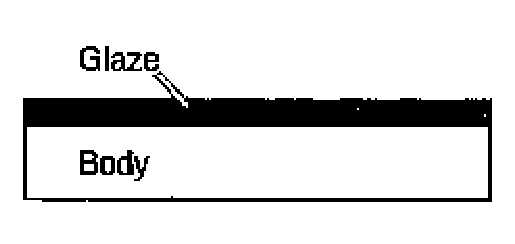
\includegraphics[width=0.6\linewidth]{img/coesame.eps}
  \caption{The body and glaze have the same coefficient of expansion.}
  \label{fig:coesame}
\end{figure}
%-------------------------------------------------------------------------------
Figure~\ref{fig:coeglaze} shows a glaze that has a higher coefficient of 
expansion (CoE) than the body.
%-------------------------------------------------------------------------------
\begin{figure}[htbp!]
  \centering
  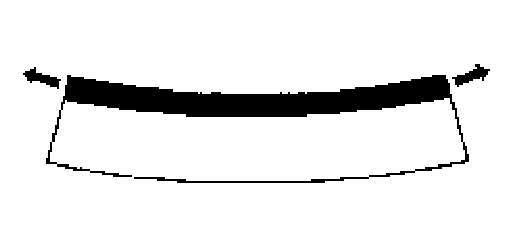
\includegraphics[width=0.6\linewidth]{img/coeglaze.eps}
  \caption{The glaze has a higher coefficient of expansion than the glaze.}
  \label{fig:coeglaze}
\end{figure}
%-------------------------------------------------------------------------------
The glaze contracted more, so it is shorter and therefore the glaze is under a 
tensile stress (it is pulled apart). If the body is very thin it will bend as 
shown. The arrows in figure~\ref{fig:coearrow} show the direction of the stress 
the glaze is under.
%-------------------------------------------------------------------------------
\begin{figure}[htbp!]
  \centering
  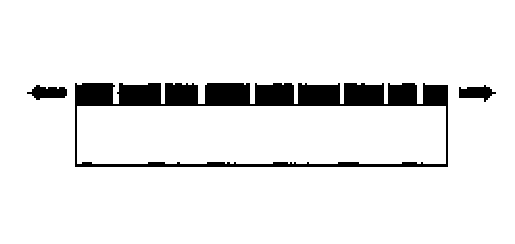
\includegraphics[width=0.6\linewidth]{img/coearrow.eps}
  \caption{Arrows show the tensile stress of a glaze which has a higher 
  coefficient of expansion than the glaze.}
  \label{fig:coearrow}
\end{figure}
%-------------------------------------------------------------------------------
More often the tensile stress is relieved by cracks in the glaze as shown in 
this figure. This is called crazing. The stress caused by high CoE of the glaze 
may be relieved by crazing as soon as the pot is taken out of the kiln or it 
may take days, months or years. The longer it takes, the closer is the CoE of 
body and glaze.
%-------------------------------------------------------------------------------
\begin{figure}[htbp!]
  \centering
  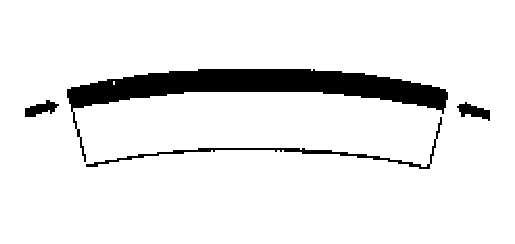
\includegraphics[width=0.6\linewidth]{img/coebody.eps}
  \caption{The body has a higher coefficient of expansion than the glaze.}
  \label{fig:coebody}
\end{figure}
%-------------------------------------------------------------------------------
Figure~\ref{fig:coebody} shows a body with higher CoE than the glaze. The body 
contracted more than the glaze. The glaze is under compression, and if the clay 
is thin it may bend as shown to relieve the pressure. If body contraction is 
only slightly greater than glaze contraction, nothing will happen as shown in 
figure~\ref{fig:coebodynothing}.
%-------------------------------------------------------------------------------
\begin{figure}[htbp!]
  \centering
  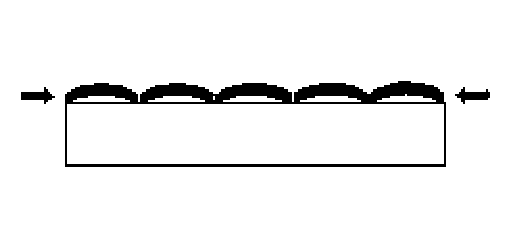
\includegraphics[width=0.6\linewidth]{img/coebodynothing.eps}
  \caption{The body has a higher coefficient of expansion, but because the body 
  contraction is only slightly greater than the glaze contraction nothing 
  happens.}
  \label{fig:coebodynothing}
5\end{figure}
%-------------------------------------------------------------------------------
If a glaze contracts much less than the body, the compression on the glaze 
becomes too much and the glaze will start to flake off (shiver) as shown in 
figure~\ref{fig:coeshiver}. This may not happen by itself, but only if 
something hits the pot. Typically, the rim of a cup will easily chip off.
%-------------------------------------------------------------------------------
\begin{figure}[htbp!]
  \centering
  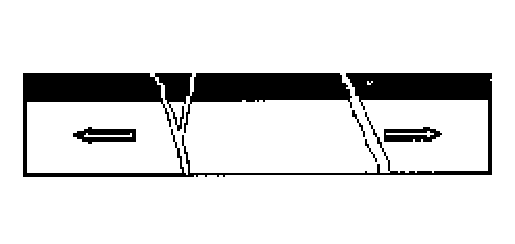
\includegraphics[width=0.6\linewidth]{img/coeshiver.eps}
  \caption{The compression on the glaze is too much and it flakes off.}
  \label{fig:coeshiver}
\end{figure}
%-------------------------------------------------------------------------------
High compression of the glaze may also be relieved by cracking of the body.
%-------------------------------------------------------------------------------
\subsubsection{Moisture Swelling}
When the body has been exposed to humidity for a long period, water enters the 
body, which expands slightly (moisture swelling). This expansion causes the 
glaze to go into tension and it will craze. This kind of crazing is called 
delayed crazing.
%-------------------------------------------------------------------------------
\subsubsection{Solutions}
As we saw above, crazing and shivering are caused by different rates of 
contraction and expansion (different CoE's). The problems are cured by 
adjusting the CoE of body and glaze, so that the two contract and expand more 
closely. It is best if the glaze is left under slight compression.
%------------------------------------------------------------------------------
\subsubsection{Coefficient of expansion}
Ceramic materials have different coefficients of expansion (CoE). 
Table~\ref{tab:coerelative} shows the relative values for the most common.
%------------------------------------------------------------------------------
\begin{center}
  \renewcommand{\arraystretch}{1.5}
  \begin{table}\centering
    \begin{tabular}{|c|c|}\hline
      \textbf{Material}&\textbf{Relative CoE}\\\hline\hline
      %------------------------------------------------------------------------------
      \ce{Na2O}&High\\\hline
      %------------------------------------------------------------------------------
      \ce{K2O}&-\\\hline
      %------------------------------------------------------------------------------
      \ce{CaO}&-\\\hline
      %------------------------------------------------------------------------------
      \ce{BaO}&-\\\hline
      %------------------------------------------------------------------------------
      \ce{TiO2}&-\\\hline
      %------------------------------------------------------------------------------
      \ce{Fe2O3}&-\\\hline
      %------------------------------------------------------------------------------
      \ce{Al2O3}&-\\\hline
      %------------------------------------------------------------------------------
      \ce{PbO}&-\\\hline
      %------------------------------------------------------------------------------
      \ce{CuO}&-\\\hline
      %------------------------------------------------------------------------------
      \ce{MnO}&-\\\hline
      %------------------------------------------------------------------------------
      \ce{ZrO2}&-\\\hline
      %------------------------------------------------------------------------------
      \ce{SnO2}&-\\\hline
      %------------------------------------------------------------------------------
      \ce{P2O5}&-\\\hline
      %------------------------------------------------------------------------------
      \ce{ZnO}&-\\\hline
      %------------------------------------------------------------------------------
      \ce{MgO}&-\\\hline
      %------------------------------------------------------------------------------
      \ce{SiO2}&-\\\hline
      %------------------------------------------------------------------------------
      \ce{B2O3}&Low\\\hline
%------------------------------------------------------------------------------ 
   \end{tabular}
    \caption{Relative coefficient-of-expansion values for common ceramic 
    materials.}
    \label{tab:coerelative}
  \end{table}
\end{center}
%------------------------------------------------------------------------------
\subsubsection{Adjusting the coefficient of expansion of a glaze}
From this list we can see that if we replace soda (\ce{Na2O}) with boron 
(\ce{B2O3}) in a glaze we will lower the CoE of the whole glaze. This can be 
done without changing the melting point of the glaze. Addition of silica will 
lower the glaze's CoE but will also raise its melting point.

If shivering occurs, it means the CoE of the glaze is too low. Adjusting it 
means adding soda (\ce{Na2O}) and reducing boron (\ce{B2O3}).
%-------------------------------------------------------------------------------
\subsubsection{Adjusting the coefficient of expansion of a body}
Adjustment of body CoE is not done according to the CoE of the materials listed 
above. The contraction rate of the body depends to a much higher degree on the 
sudden reversible contraction of silica crystals when these change their 
crystal structure (cristobalite).
%-------------------------------------------------------------------------------
\subsubsection{Quartz change}
Quartz is a crystal form of silica. Quartz is created in the body during firing 
when the clay crystal changes form and releases some of its silica. When quartz 
is heated it changes its crystal structure at 573\degree C. This happens very 
suddenly and is accompanied by a 1\% expansion. On cooling to below 573\degree 
C it contracts again. See figure~\ref{fig:quartzinversion} for a visual 
depiction of this change.
%-------------------------------------------------------------------------------
\begin{figure}[htbp!]
  \centering
  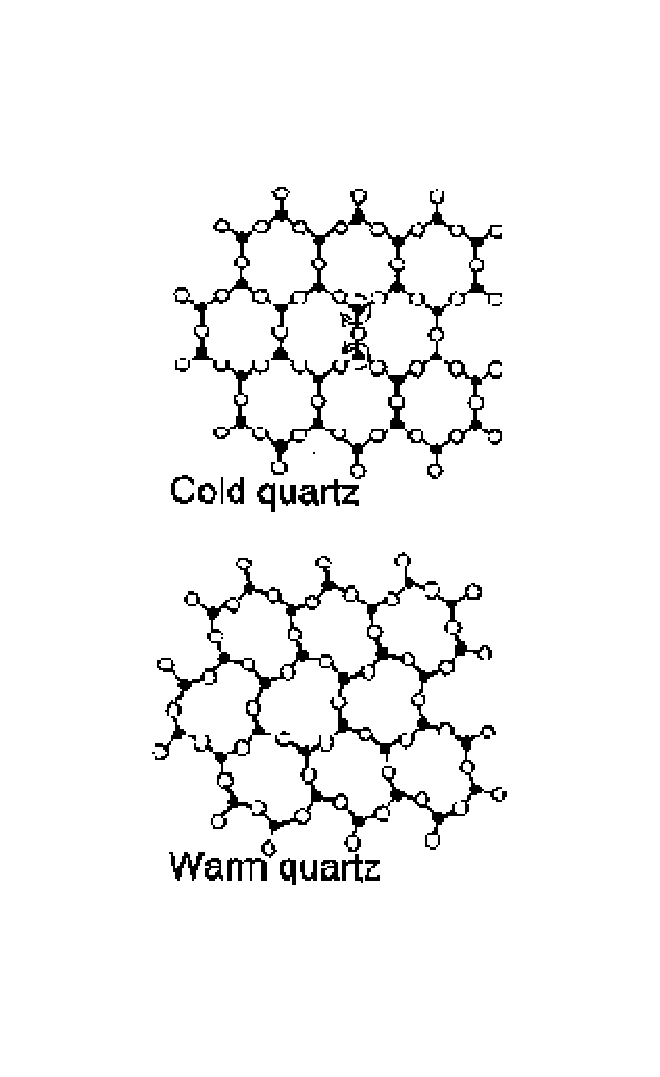
\includegraphics[width=0.6\linewidth]{img/quartzinversion.eps}
  \caption{The volume change of quartz is caused by a rearrangement of the bond 
  between the atoms. At 573\degree C the angle suddenly shifts as shown.}
  \label{fig:quartzinversion}
\end{figure}
%-------------------------------------------------------------------------------
\subsubsection{Cristobalite}
Cristobalite is another crystal form of silica. It changes its size around 
220\degree C and the volume change is nearly 3\%. Cristobalite is created at 
temperatures above 900\degree C from silica released from the clay 
(\ce{Al2O3*2SiO2}) or talc (\ce{3MgO*4SiO2}) or from quartz.
%-------------------------------------------------------------------------------
\begin{figure}[htbp!]
  \centering
  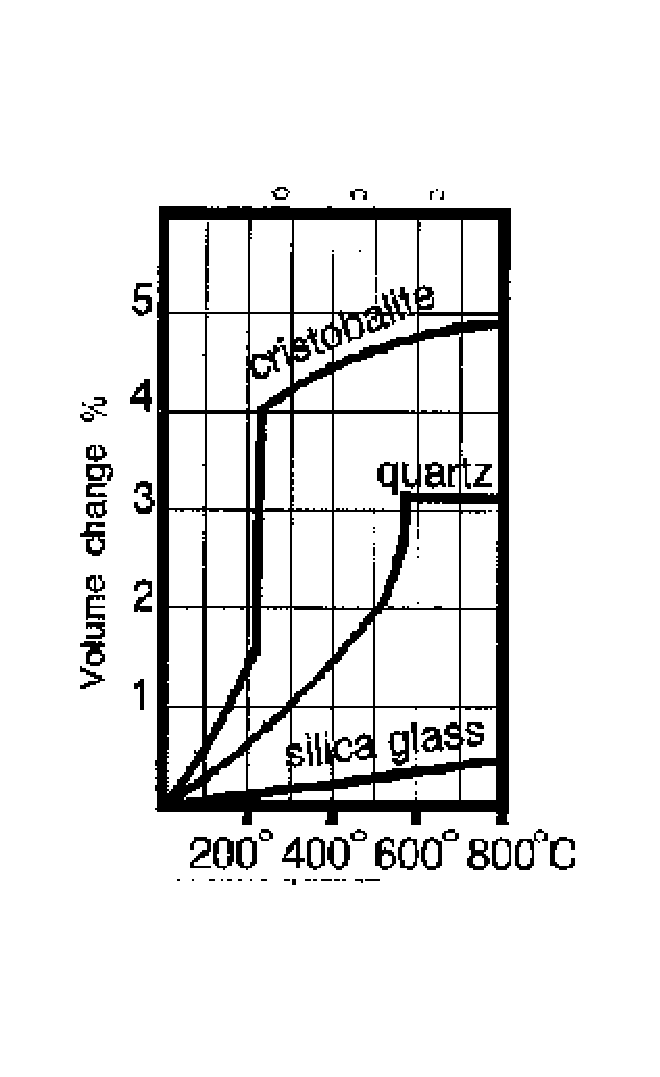
\includegraphics[width=0.6\linewidth]{img/cristobalite.eps}
  \caption{The graph shows volume changes of three forms of silica. The two 
  crystal forms change dramatically but silica in glass hardly changes.}
  \label{fig:cristobalite}
\end{figure}
%-------------------------------------------------------------------------------
\subsubsection{Body-glaze contraction}
The two graphs below show how the body and its glaze contract during cooling. 
The graph in figure~\ref{fig:bodyglazewithout} shows a body that does 
not contain any cristobalite. At 573\degree C the body contracts suddenly due 
to the contraction of quartz, but at this temperature the glaze is still fluid 
enough to follow the contraction of the body.

Around 500\degree C the earthenware glaze hardens and from then onwards 
contracts according to its own CoE. In this example the glaze has a higher CoE 
than the body; it contracts more. This leaves the glaze under tensile stress; 
the glaze is smaller than the body. This will cause the glaze to craze.

The graph in figure~\ref{fig:bodyglazewith} shows contraction of a body 
containing cristobalite. As above, the glaze first follows the quartz 
contraction, then hardens and starts to contract more than the body. However, 
at 220\degree C the cristobalite change causes the body to contract, and at 
this 
temperature the glaze is hard so it is left under compression. This compression 
will prevent the glaze from crazing.
%-------------------------------------------------------------------------------
\begin{figure}[htbp!]
  \centering
  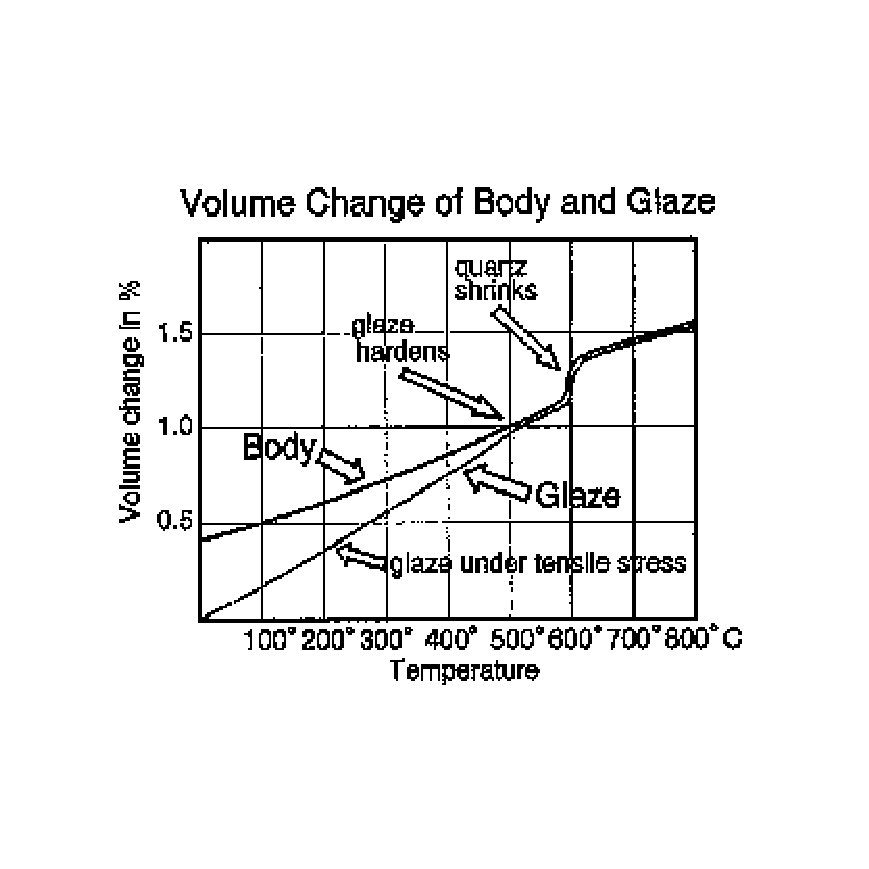
\includegraphics[width=0.6\linewidth]{img/bodyglazewithout.eps}
  \caption{Contraction of body and glaze during cooling. The glaze contracts 
  more 
  so it will craze.}
  \label{fig:bodyglazewithout}
\end{figure}
%-------------------------------------------------------------------------------
\begin{figure}[htbp!]
  \centering
  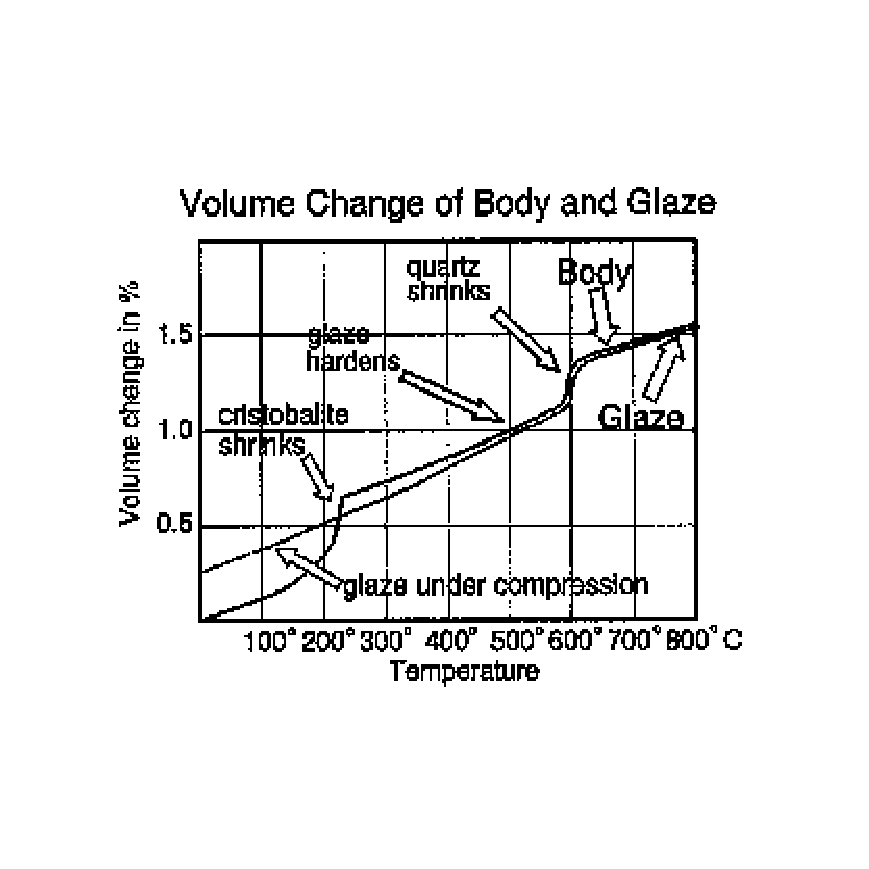
\includegraphics[width=0.6\linewidth]{img/bodyglazewith.eps}
  \caption{The body in this graph contains crisotobalite and shows a sudden 
  contraction at 220\degree C. This causes an overall higher contraction of 
  body compared to glaze.}
  \label{fig:bodyglazewith}
\end{figure}
%-------------------------------------------------------------------------------
\subsubsection{Moisture crazing}
After firing, the porous earthenware body will absorb moisture and this causes 
the body to expand. If the glaze is not under sufficient compression it will 
craze. Such delayed crazing may occur a long time after firing. The moisture 
expansion of the body is reduced by making the body more vitreous. Additions of 
talc or limestone to the body reduce moisture crazing.
%-------------------------------------------------------------------------------
\subsubsection{Crazing cure}
For both types of crazing the cure is:
%-------------------------------------------------------------------------------
\begin{itemize}
\item Add quartz (or silica), talc or limestone to the body.
\item Biscuit-fire to a higher temperature.
\item Glaze-fire to a higher temperature.
\item Add silica to the glaze.
\item In the glaze, replace fluxes with high thermal expansion, like soda 
(\ce{Na2O}) and potash (\ce{K2O}), with boron oxide (\ce{B2O3}).
\end{itemize}
It may seem strange that the cure for crazing is to add silica to both body and 
glaze. The reason is that adding silica to glaze makes it contract less, but 
silica added to the body causes the body to contract more.
%-------------------------------------------------------------------------------
\subsubsection{Crazing test}
There are several ways to test how the expansion of glaze and body fit each 
other. The most simple ones are:
%-------------------------------------------------------------------------------
\begin{itemize}
\item Rings of clay with a diameter of 5 to 10 cm are made with a small gap and 
biscuit. The gap is measured, the ring is glazed on its outer surface and 
refired. After firing the gap is measured to see if the ring has contracted or 
expanded. If the gap has become greater the glaze will craze.
\item Glazed samples are exposed to thermal shocks by repeated heating and 
cooling.
\end{itemize}
%-------------------------------------------------------------------------------
The thermal shocks can be from boiling water into ice water. The number of 
cycles the sample can withstand before crazing indicates its craze resistance.

Another method is to heat the sample at first to 100\degree C then cool it in 
20\degree C water. This is repeated while raising the temperature in steps of 
10 or 20 degrees. The higher the heating temperature the sample withstands 
without crazing the longer it will be able to stay craze-free under normal 
conditions.

A rough guide is:
%-------------------------------------------------------------------------------
\begin{itemize}
\item 120\degree C: craze-free for 8 days
\item 150\degree C: craze-free for 100 days
\item 180\degree C: craze-free for 2 years
\item 200\degree C: craze-free for life
\end{itemize}
%-------------------------------------------------------------------------------
Even if a sample survives the thermal shock test it may still craze due to 
moisture swelling. This can be tested in an autoclave which is simply a 
pressure cooker that can withstand higher pressures. A pressure cooker can be 
used instead. The glaze sample is placed in the pressure cooker with some 
water. It is kept under pressure for a period and then checked for crazing. The 
time it can withstand pressure without crazing indicates the time it may stay 
craze-free under normal circumstances. 

Table~\ref{tab:autoclave} is a rough guide for testing in an autoclave under a 
pressure of 3 atmospheres (about 3 bars). If using a pressure with, say, a 
pressure of 1.5 atmospheres the testing time in the table should be doubled.

All the tests provide only a rough indication of craze resistance. When you do 
the test you will develop your own procedure' which then should always be 
followed faithfully. In this way you will be able to compare your crazing test 
with your previous results.
%------------------------------------------------------------------------------
\begin{center}
  \renewcommand{\arraystretch}{1.5}
  \begin{table}\centering
    \begin{tabular}{|c|c|}\hline
      \textbf{Hours in autoclave}&\textbf{Expected craze-free 
      life}\\\hline\hline
      %------------------------------------------------------------------------------
      1&1--2 years\\\hline
      %-----------------------------------------------------------------------------
      2&2--3 years\\\hline
 %-----------------------------------------------------------------------------
      3&4--6 years\\\hline
%-----------------------------------------------------------------------------
      4&9--10 years\\\hline
%-----------------------------------------------------------------------------
      5&13--15 years\\\hline
%-----------------------------------------------------------------------------
    \end{tabular}
    \caption{A rough guide to testing for crazing in an autoclave.}
    \label{tab:autoclave}
  \end{table}
\end{center}
%-------------------------------------------------------------------------------
\subsection{Crawling}
Crawling appears as areas of clay that are not covered by the glaze. It may be 
small areas or, in extreme cases, the glaze may pull up into a pattern of small 
balls or islands, leaving bare clay in between.

Crawling is caused by:
%-------------------------------------------------------------------------------
\begin{itemize}
\item Poor adhesion of glaze:

Dusty or oily biscuit prevents the glaze from sticking to the body. Refractory 
oxides (chrome, rutile) or underglazes that act as a dust layer prevent the 
formation of an interface. Adding clay, borax or frit to the underglaze 
colorants helps.

\item High surface tension:

High surface tension of the glaze in melting pulls it into islands before the 
clay/glaze interface forms. This is caused by certain oxides, especially 
magnesia, clay and zinc oxide. The solution is to replace magnesia by other 
materials, to calcine part of the clay or to use calcined zinc oxide instead of 
raw.

\item Cracking of glaze layer:

Extensive shrinkage of glaze in drying and early stages of firing, usually 
caused by too much clay content or by overgrinding the glaze, causes the glaze 
to crack and separate from the body. A thick glaze layer is more likely to 
crack.
\end{itemize}
%-------------------------------------------------------------------------------
\subsection{Pinholing and Blistering}
Pinholes appear as tiny holes in the glaze surface. Blisters look like frozen 
bubbles or craters. They are a problem in utilitarian ware, as they collect 
dirt. They may be only on the surface of the glaze or may penetrate to the clay 
layer.

During firing gas bubbles are formed in the melted glaze. The bubbles will move 
to the surface of the fluid glaze and be released.

If you watch any glaze melting, you can actually see this process. Some glazes 
(especially those containing raw borax) foam and boil until they finally smooth 
out. When the firing is stopped before the glaze has had time to heal over, a 
pinhole or crater is left (see figure~\ref{fig:pinholing}). Since overfiring 
also causes pinholes it is better to keep the maximum temperature for some time 
(soaking period).

%-------------------------------------------------------------------------------
\begin{figure}[htbp!]
  \centering
  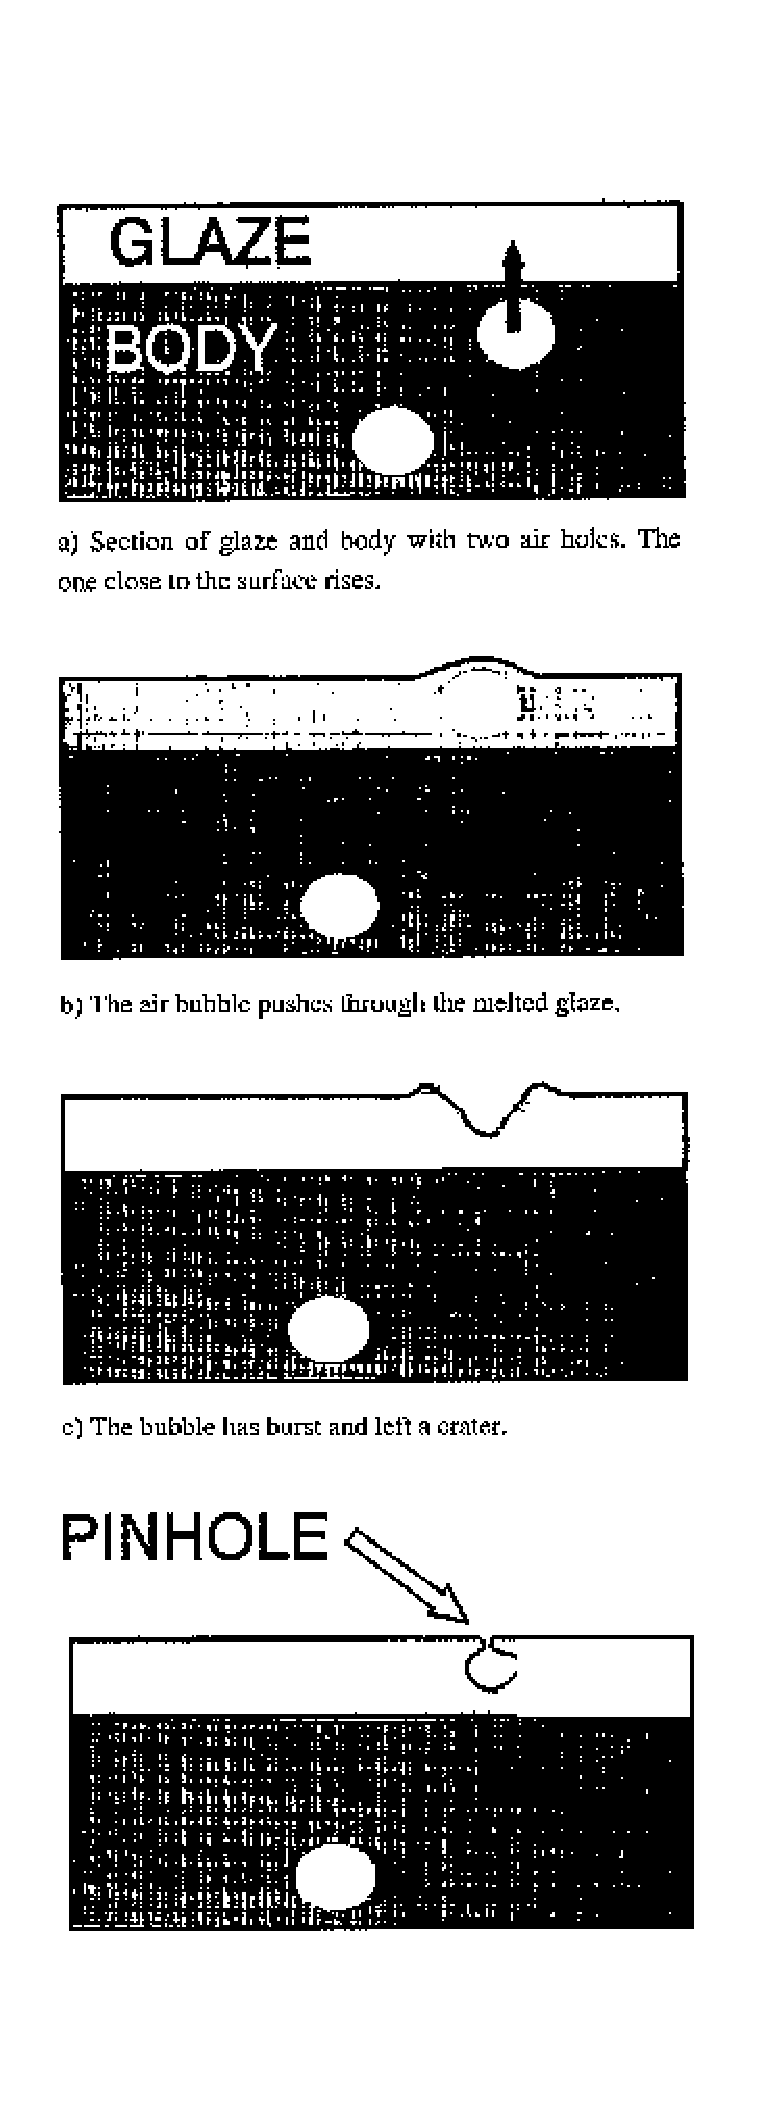
\includegraphics[width=0.6\linewidth]{img/pinholing.eps}
  \caption{How pinholes form in a glaze.}
  \label{fig:pinholing}
\end{figure}
%-------------------------------------------------------------------------------
The main sources of the gas are:
%-------------------------------------------------------------------------------
\begin{itemize}
\item After glazing, a large volume of air exists in the space between the 
solid glaze materials. The air gathers into bubbles during sintering and 
melting.
\item Release of sulfates and carbon in the body and from some of the glaze 
materials.
\item Air bubbles in the body introduced by improper handling of the casting 
slip.
\item Sulfates and carbon from the fuel may deposit in the body during the 
initial stages of firing. Above 900\degree C the gas will be released.
\end{itemize}
%-------------------------------------------------------------------------------
It is important to find out if the problem is in the glaze or in the body. 
Relatively large pinholes that go all the way to the body are usually caused by 
small holes in the body that do not accept the glaze-this is most common with 
slip-cast ware, or with common red clay that contains particles of organic 
matter, sand or mica.

Problems arise if the glaze starts to cool and solidify while bubbles or 
craters are still forming.

Detailed causes and solutions are given in section~\ref{sec:problemmelt}.
%-------------------------------------------------------------------------------
\subsection{Color Changes}
Potters are often plagued by changes in glaze color, either within the same 
kiln-load or from separate firings.

Often this problem can be traced to glaze preparation. The colors may not be 
ground finely enough, weighing may be incorrect, raw materials may have changed.

Otherwise, the problem usually is due to more or less reduction than usual. 
This is one of the most difficult conditions to control in firing and depends 
completely on the skill of the firemaster.

The problem is worst in glazes that contain color oxides that are sensitive to 
reduction. The most sensitive is copper, which is green in oxidation and red in 
reduction; and iron oxide, which is yellow, red to brown in oxidation and 
mottled red-brown, grey to blue or green in reduction. Other oxides change less.

Heavy reduction will darken the iron in the body, which will affect the glaze, 
also darkening it. Sometimes a pot will be dark on the reduced side and light 
on the oxidized side.

Other causes and solutions are given above.
%-------------------------------------------------------------------------------
\chapter{Developing Glazes}
Most potters do not know much about glaze chemistry and are usually afraid to 
develop their own glazes. It is true that glaze chemistry is difficult to 
understand without a background in chemistry. Still, a simple knowledge of 
fluxes, stabilizers and glass formers and how they combine to make glaze is 
useful. It will give even the nontechnical potter an idea of how to approach 
glaze problems and develop new colors and textures. The reader with more 
technical background can make use of the Seger formula for a more sophisticated 
approach to glazes.

Remember that glaze chemistry is something new in the history of ceramics. 
Before it existed, potters found out how to make glazes by trial and error, 
without modern methods of analysis or even accurate methods of weighing.

It is also true that once glaze recipes were developed they were closely 
guarded secrets. A special glaze that no one else could duplicate gave an 
advantage over the competition. The modern systematic, scientific approach to 
glaze development has largely made ``secret'' glazes obsolete because the 
action of the various glaze ingredients is now well known.

On the other hand, glaze making is very much like cooking. The same recipe may 
produce very different results when prepared by two different cooks! Standard 
glaze recipes as published in books often do not work because of differences in 
raw materials, firing technique etc. Just as a good cook should know how to 
substitute materials, a good glaze maker can develop an intuitive knowledge of 
glazes. Like most things, this only comes from hard-won experience.

Potters should not be afraid to experiment with glaze development, although 
most of them simply do not have the time to take away from production. The 
following chapters describe standard approaches to glaze development and will 
be useful to those who want to experiment with glazes.
%------------------------------------------------------------------------------
\section{Modifying Existing Glazes}
The easiest approach to working with glazes is to start by modifying existing 
glazes. These may be new recipes from books, or recipes that you are already 
using. Although you can take a trial-and-error approach, this takes a lot of 
time and money, and results are largely a matter of luck. It is best to use 
some of the systematic methods presented below and knowing even a little about 
the nature of the various glaze materials will help you reach your goal more 
efficiently.

There are three approaches to modifying glazes:
%------------------------------------------------------------------------------
\begin{itemize}
\item You have a goal for a particular surface, color, texture etc.
\item You have a glaze problem that needs to be corrected.
\item You have no special goal but just want to see what happens when you 
change the recipe.
\end{itemize}
%------------------------------------------------------------------------------
\section{Basic Equipment}
The minimum equipment required for glaze testing is:
%------------------------------------------------------------------------------
\begin{itemize}
\item Accurate balance, either a triple beam balance or a goldsmith's balance 
with weight. Spring-type scales are not accurate enough for weighing glazes.
\item A mortar and pestle for grinding materials. These should be porcelain, so 
that they do not contaminate tests.
\item A 100-mesh sieve. This can be bought ready-made, or you can make your own 
using brass or stainless steel screen.
\item Firing can be done in your regular glaze firing.
\end{itemize}
%------------------------------------------------------------------------------
\section{Testing Methods}
\subsection{Test Pieces}
The type of test piece you use is largely a matter of personal preference. In 
order to show glaze behavior under various circumstances, it should have:
%------------------------------------------------------------------------------
\begin{itemize}
\item A horizontal and vertical surface.
\item A textured area.
\item A hole to tie it. This helps to keep similar tests together for future 
reference.
\item An area for labeling. It is best to write the full recipe of the test on 
each test tile (with a brush and iron oxide and water, or chrome oxide or 
engobe etc.) since code numbers often get confused and notebooks get lost.
\end{itemize}
%------------------------------------------------------------------------------
The first step in understanding your materials is to fire all available 
materials in small bowls at your standard glaze firing temperature.

A small quantity of each material (ground and sieved through 100 mesh) is 
placed dry in the bowl. This will show you which ones melt alone, and which 
ones remain as powder. Most of the materials will not melt but may change in 
color or may react with the clay. Only the strong fluxes will melt by 
themselves -other materials that do not melt may be fluxes, but only in 
combination with other materials.
%------------------------------------------------------------------------------
\subsection{Line Blending}
Line blending is a systematic way of finding out the reactions of two different 
materials (or mixtures of materials).

The easiest way is to prepare the two materials by grinding, sieving and mixing 
them with water in two separate containers. To make the line blend, the 
materials are mixed by volume (using a small spoon) and applied on a test tile, 
starting with one material alone and adding the other material in equal steps. 
Since the tests are measured by volume it is important that the same amount of 
water is added to the two line blend materials.

Glaze half of the test tile twice to show variation in glaze thickness.

An example of a line blend in 10 steps, which gives the full range of 
combinations of 2 materials, is shown in table~\ref{tab:lineblend10}.

The most common use of the line blend is to find out the effect of one material 
in a standard glaze recipe. If material A is the standard glaze recipe, 
material B could be the standard glaze + a coloring oxide addition of 5-10%.

Usually, 5 steps will be enough for the first test. In 
table~\ref{tab:lineblend5ox}, material A is the basic glaze, material B is the 
basic glaze + 10\% copper oxide.
%------------------------------------------------------------------------------
\begin{center}
  \begin{table}\centering
  \renewcommand{\arraystretch}{1.5}    
  \begin{tabular}{|c||c|c|c|c|c|c|c|c|c|c|c|}\hline
      \textbf{Material}
      &\multicolumn{11}{c}{\textbf{Parts by volume}}\vline\\\hline\hline
      Material A&0&1&2&3&4&5&6&7&8&9&10\\\hline
      Material B&10&9&8&7&6&5&4&3&2&1&0\\\hline
    \end{tabular}
  \caption{A line blend of 10 steps.}
\label{tab:lineblend10}
  \end{table}
\end{center}
%------------------------------------------------------------------------------
\begin{center}
  \renewcommand{\arraystretch}{1.5}
  \begin{table}\centering
    \begin{tabular}{|c||c|c|c|c|c|c|}\hline
      \textbf{Material}&\multicolumn{6}{c}{\textbf{Parts by 
      volume}}\vline\\\hline\hline
      \textbf{Test}
    &\textbf{A}&\textbf{B}&\textbf{C}&\textbf{D}&\textbf{E}&\textbf{F}\\\hline\hline
      Glaze A&0&2&4&6&8&10\\\hline
      Glaze A + 10\% \ce{CuO}&10&8&6&4&2&0\\\hline
      \ce{CuO} in test&10\%&8\%&6\%&4\%&2\%&0\%\\\hline
     \end{tabular}
    \caption{A line blend of 5 steps, mixing glazes and an oxide.}
    \label{tab:lineblend5ox}
  \end{table}
\end{center}
%------------------------------------------------------------------------------
\subsubsection{Mixing procedure}
\begin{enumerate}
\item First prepare a line blend mixing card like the one above.
\item Prepare the two mixtures as usual and add the same amount of water to 
each.
\item Place the two materials in bowls in front of you, glaze A to your left 
and glaze B to your right.
\item In the middle place an empty bowl into which you pour the spoonfuls from 
the two other bowls according to the number for each test on your line blend 
card. Keep track of the spoon counting by marking the line blend card.
\item Stir the test mixture well.
\item Mark a test tile with the mixture's test number (date + serial number).
\item Glaze the test tile.
\item Discard the remaining glaze and continue with the other line blend 
mixtures.
\end{enumerate}

\subsubsection{Calculation example}
In the case above it was easy to calculate the copper oxide addition in each of 
the tests. When more complex mixtures are used in a line blend the calculation 
becomes more complicated. 

Table~\ref{tab:lineblend5} shows an example of mixing two glazes of the 
following compositions:
\begin{itemize}
\item Glaze A:
\begin{itemize}
\item Frit X: 70
\item Feldspar: 15
\item Quartz: 5
\item Kaolin: 10
\end{itemize}
\item Glaze B
\begin{itemize}
  \item Frit Y: 80
  \item Zircon: 10
  \item Kaolin: 10
\end{itemize}
\end{itemize}
%------------------------------------------------------------------------------
\begin{center}
  \renewcommand{\arraystretch}{1.5}
  \begin{table}\centering
    \begin{tabular}{|c||c|c|c|c|c|c|}\hline
      &\multicolumn{6}{c}{\textbf{Parts by volume}}\vline\\\hline\hline
      \textbf{Test Number}
      &\textbf{A}&\textbf{B}&\textbf{C}&\textbf{D}&\textbf{E}&\textbf{F}\\\hline\hline
      Glaze A&0&2&4&6&8&10\\\hline
      Glaze B&10&8&6&4&2&0\\\hline
    \end{tabular}
    \caption{A line blend of 5 steps.}
    \label{tab:lineblend5}
  \end{table}
\end{center}
%------------------------------------------------------------------------------
After firing, Test D turned out to be the most interesting. We now want 
to test a larger amount of this and the recipe is calculated as shown in 
table~\ref{tab:lineblendtestd}.

The sums of each material were then divided by 5 and the final recipe is shown 
in table~\ref{tab:lineblendglazed}.

The recipe is based on a line blend test measured by spoonfuls. That is not 
very accurate so, before going any further, the test result should be retested 
by weighing the dry materials.
%------------------------------------------------------------------------------
\begin{landscape}
  \begin{center}
  \renewcommand{\arraystretch}{1.5}
  \begin{table}\centering
    \begin{tabular}{|c||c|c|c|c|c|c|c|}\hline
      &\textbf{Parts}&\textbf{Frit X}&\textbf{Frit 
      Y}&\textbf{Feldspar}&\textbf{Quartz}&\textbf{Zircon}&\textbf{Kaolin}\\\hline\hline
      Glaze A&3&210&0&45&15&0&30\\\hline
      Glaze B&2&0&160&0&0&20&20\\\hline
      Total A+B&5&210&160&45&15&20&50\\\hline\hline
      New Glaze D&0.2&42&32&9&3&4&10\\\hline
    \end{tabular}
    \caption{The composition of Test D. Materials in Glaze A were multiplied by 
    3, and Glaze B by 2.}
    \label{tab:lineblendtestd}
  \end{table}
\end{center}
\end{landscape}
%------------------------------------------------------------------------------
\begin{center}
  \renewcommand{\arraystretch}{1.5}
  \begin{table}\centering
    \begin{tabular}{|c|c|}\hline
      \textbf{Ingredient}&\textbf{Percent}\\\hline\hline
      Frit X&42\%\\\hline
      Frit Y&32\%\\\hline
      Feldspar&9\%\\\hline
      Quartz&3\%\\\hline
      Zircon&4\%\\\hline
      Kaolin&10\%\\\hline
    \end{tabular}
    \caption{Glaze D, final recipe.}
    \label{tab:lineblendglazed}
  \end{table}
\end{center}
%------------------------------------------------------------------------------
\subsection{Triaxial Blending}
Triaxial blending is a method of testing varying amounts of three different 
materials or colors.
%-------------------------------------------------------------------------------
\begin{figure}[htbp!]
  \centering
  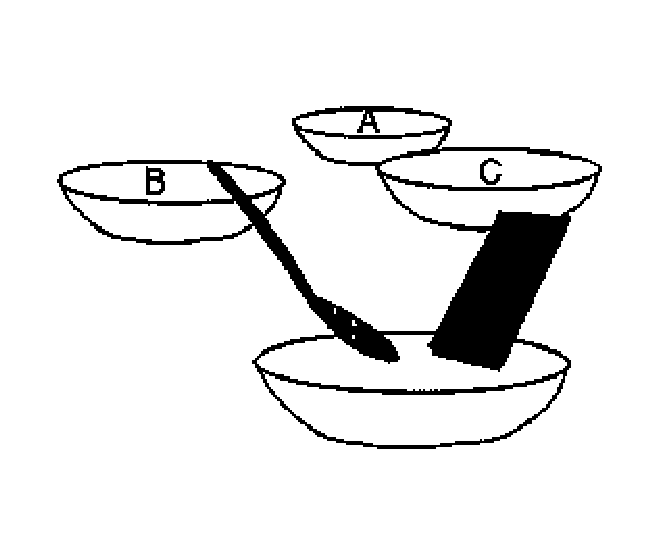
\includegraphics[width=0.7\linewidth]{img/triaxialbowls.eps}
  \caption{Arrangement of bowls for triaxial mixing.}
  \label{fig:triaxialbowls}
\end{figure}
%-------------------------------------------------------------------------------
\begin{figure}[htbp!]
  \centering
  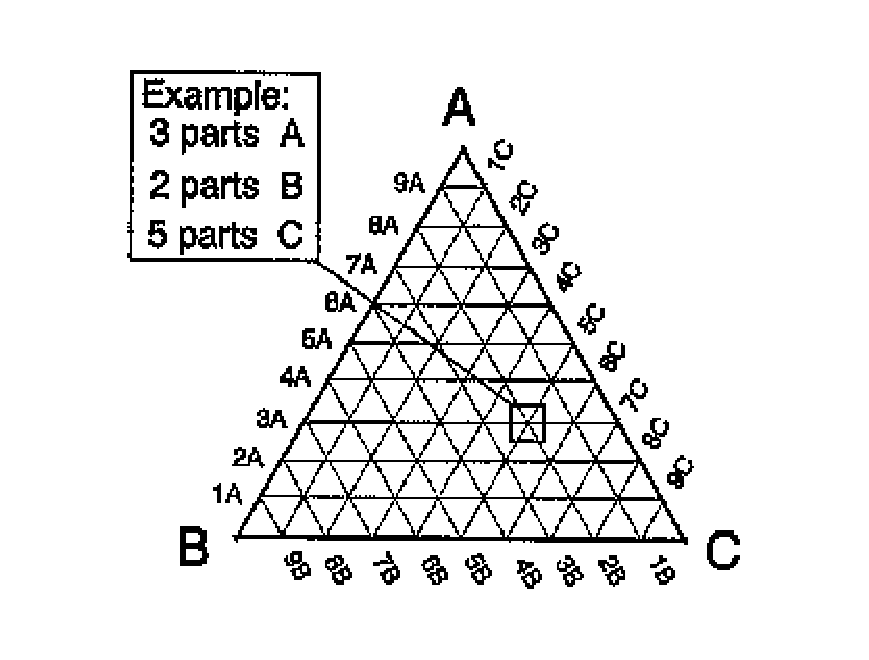
\includegraphics[width=0.7\linewidth]{img/triaxial10.eps}
  \caption{A triaxial blending chart system with 10 steps. Composition of a 
    test at an intersection is found by following the lines to the periphery of 
    the triangle.}
  \label{fig:triaxial10}
\end{figure}
%-------------------------------------------------------------------------------
\begin{figure}[htbp!]
  \centering
  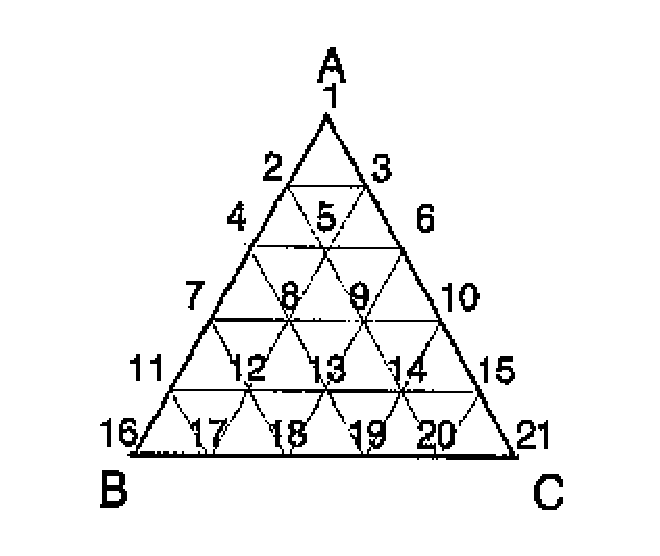
\includegraphics[width=0.7\linewidth]{img/triaxial5.eps}
  \caption{Triaxial system with 5 steps. The number at each point refers to the 
    test number on the triaxial blending card.}
  \label{fig:triaxial5}
\end{figure}
%-------------------------------------------------------------------------------
Each corner of the triangle represents 100\% of the material. Each side of the 
triangle is the line blend of the materials at its ends, and the intersections 
inside the triangle represent combinations of all three materials. So the 
result is three line blends, plus all the combinations. 

Figure~\ref{fig:triaxial10} is an example of a biaxial system with 66 tests.

The system is better explained by an example. You may have a basic opaque glaze 
and you want to see how it responds to 3 different coloring oxides: cobalt 
oxide, copper oxide and iron oxide. In this case we use a simple biaxial blend 
with only 21 tests as shown in figure~\ref{fig:triaxial5}.

The procedure is:
%-------------------------------------------------------------------------------
\begin{itemize}
\item Prepare a biaxial blending card as shown.
\item Prepare 3 mixtures of basic glaze with oxide additions:
%-------------------------------------------------------------------------------
\begin{itemize}
\item A glaze + 5\% cobalt oxide
\item B glaze + 10\% iron oxide
\item C glaze + 10\% copper oxide
\end{itemize}
%-------------------------------------------------------------------------------
\item Add same amount of water, screen 100 mesh.
\item Place 3 bowls with the mixtures in front of you: B on the left, C on the 
right, A in the center. Right in front of you place an empty bowl. See 
figure~\ref{fig:triaxialbowls}
\item Have all test tiles numbered and arranged in sequence near by.
\item Collect teaspoonfuls of each mixture; A, B, C according to the numbers on 
the biaxial card. Mark each time you have finished collecting from each bowl.
\item The mixture is collected in the empty bowl.
\item Stir the mixture, pick the test tile with the right biaxial blend number.
\item Glaze the test tile.
\end{itemize}
%-------------------------------------------------------------------------------
Getting the right number of spoonfuls into the collection bowl for each test 
takes a lot of concentration. A mixing card as shown in 
table~\ref{tab:mixingcard} helps you to keep track of your progress with the 
spoon counting.
%-------------------------------------------------------------------------------
\begin{landscape}
\begin{center}
  \begin{table}\centering
  \renewcommand{\arraystretch}{1.5}
  \begin{tabular}{|c||c|c|c|c|c|c|c|c|c|c|c|c|c|c|c|c|c|c|c|c|c|}\hline
    &\multicolumn{21}{c}{\textbf{Triaxial Blending Card}}\vline\\\hline\hline
    \textbf{Test Number}
    &\textbf{1}&\textbf{2}&\textbf{3}&\textbf{4}&\textbf{5}&\textbf{6}
    &\textbf{7}&\textbf{8}&\textbf{9}&\textbf{10}&\textbf{11}&\textbf{12}&\textbf{13}
    &\textbf{14}&\textbf{15}&\textbf{16}&\textbf{17}&\textbf{18}&\textbf{19}
    &\textbf{20}&\textbf{21}\\\hline\hline
    Material&\multicolumn{21}{c}{Number of Spoonfulls}\vline\\\hline\hline
    Mixture A&5&4&4&3&3&3&2&2&2&2&1&1&1&1&1&0&0&0&0&0&0\\\hline
    Mixture B&0&1&0&2&1&0&3&2&1&0&4&3&2&1&0&5&4&3&2&1&0\\\hline
    Mixture C&0&0&1&0&1&2&0&1&2&3&0&1&2&3&4&0&1&2&3&4&5\\\hline
  \end{tabular}
  \caption{A blending card for a triaxial blend.}
  \label{tab:mixingcard}
\end{table}
  \end{center}
\end{landscape}
%-------------------------------------------------------------------------------
If you want to know the recipe of one of the tests, say number 14, you 
calculate this in the same way as for line blends. See 
table~\ref{tab:lineblend14}. Once you get used to working with biaxial blends, 
you will be able to read the percentage directly from the triangular chart.

This biaxial blend was based on only 21 variations. Out of these only 6 were 
blendings of all three mixtures; the rest were simply line blends involving 
only two mixtures. A larger biaxial blend system would produce more intermixing 
of all three materials, but also a lot of extra work. However, you could use a 
system with 10 steps on each side as shown in 
figure~\ref{fig:glazetestrecordform}, but leaving out the line blends A--B, 
A--C and B--C, and only blend the 36 
tests in the center of the triangle.
%-------------------------------------------------------------------------------
\begin{figure}[htbp!]
  \centering
  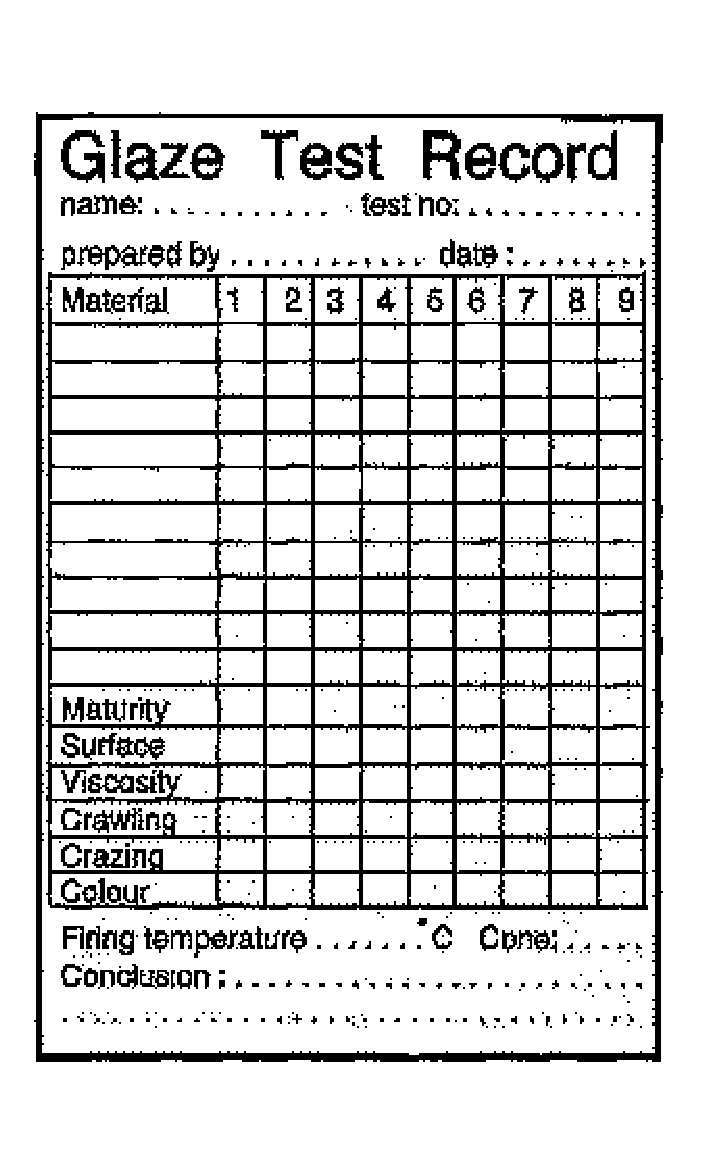
\includegraphics[width=0.45\linewidth]{img/glazetestrecordform.eps}
  \caption{Example of a glaze test record form.}
  \label{fig:glazetestrecordform}
\end{figure}
%-------------------------------------------------------------------------------
\begin{landscape}
  \begin{center}
\begin{table}\centering
    \renewcommand{\arraystretch}{1.5}
\begin{tabular}{|c||c|c|c|c|c|c|}\hline
&&\textbf{Parts}&\textbf{Glaze}&\textbf{Cobalt Oxide}&\textbf{Iron 
Oxide}&\textbf{Copper Oxide}\\\hline\hline
\textbf{Mixture A}&1&100&5&0&0&0\\\hline
\textbf{Mixture B}&1&100&0&0&10&0\\\hline
\textbf{Mixture C}&3&300&0&0&0&30\\\hline
\textbf{Total}&-&5&500&5&10&30\\\hline
\textbf{Recipe D}&Total/5&100\%&+1\%&0&+2\%&+6\%\\\hline
\end{tabular}
  \caption{A line blend of test number 14.}
\label{tab:lineblend14}
\end{table}
\end{center}
\end{landscape}
%-------------------------------------------------------------------------------
\subsection{Keeping Records}
The key to experimenting with glazes is keeping accurate records and labeling 
them in such a way that the actual tests can be compared with your notebook.

As mentioned above, it is best to write the entire recipe on the test tile 
itself, along with the date of testing. This is possible with a simple test 
like adding coloring oxides to your basic glaze. For more complicated tests and 
line blend or biaxial blend tests, you will have to rely on the test number on 
the tile. Mark the date, the number and, if you do more than one test a day, 
add a serial number. In your notebook, the date and recipe are also written.

Make it a habit to take notes of the fired results immediately after unloading 
the kiln. Write down firing conditions, location of test tile in the kiln, and 
your impression of the glaze. Is it well melted, running, pinholes or tendency 
to crawl? Use a whole sheet of paper for each test or test series. Finally 
write down your conclusion like ``make 1 kg test batch'', ``test again with 5\% 
increase of clay''.

Testing is costly and the records help you to avoid unnecessary tests. When 
planning your next test, first take a look at your earlier results and compare 
them with your notes. When deciding which materials to add or which to decrease 
you may check with the oxide list (see section~\ref{sec:glazeoxides}). As long 
as you work with one particular problem or line of research keep the test tiles 
close by for easy reference. Once you have finished the research you can store 
all the tests together by hanging them on a string in chronological order.
%-------------------------------------------------------------------------------
\section{Developing a Base Glaze}
The first step in developing a new glaze is to develop a base glaze, which is 
simply the combination of materials that melts at the desired temperature 
(without addition of colorants). Here, we describe an approach to making base 
glazes without knowing anything about the chemical composition of the materials.

Since all glazes require flux, stabilizer and glass former, these three 
materials are the starting point. There are a large number of fluxes available 
(divided into primary and secondary' fluxes), but the stabilizer is usually 
china clay (kaolin) and the glass former is usually quartz (silica). The main 
differences are between low temperature and high temperature glazes. Below only 
the main materials (not chemicals) are mentioned. This list is a rough guide 
only.

\subsection{Low Temperature Glazes (900--1100\degree C)}
Low temperature glazes require more flux and stronger flux than high 
temperature ones.

Primary Fluxes:
\begin{itemize}
\item Red Lead
\item White Lead
\item Borax or boric acid
\item Soda ash
\item Gerstley borate (calcium borate)
\item Frit (lead, borax, led borosilicate)
\end{itemize}

Secondary fluxes:
\begin{itemize}
\item Zinc oxide
\item Barium carbonate
\item Limestone
\item Marble dust
\item Talc
\end{itemize}

Stabilizer:
\begin{itemize}
\item China clay
\item Other clay
\end{itemize}

Glass former:
\begin{itemize}
\item Quartz
\item Window glass powder
\end{itemize}

\subsection{High Temperature Glazes (1100--1300\degree C)}
Low temperature glazes require more flux and stronger flux than high 
temperature ones.

Primary Fluxes:
\begin{itemize}
  \item Feldspar
  \item Nepheline syenite
  \item Fusible clay
  \item Wood ash
\end{itemize}

Secondary fluxes:
\begin{itemize}
  \item Zinc oxide
  \item Barium carbonate
  \item Limestone
  \item Marble dust
  \item Talc
\end{itemize}

Stabilizer:
\begin{itemize}
  \item China clay
  \item Other clay
\end{itemize}

Glass former:
\begin{itemize}
  \item Quartz
\end{itemize}

In the appendix there is a selection of glazes that can be used as a starting 
point for developing new glazes.

\subsection{Selection of Materials}
Materials necessarily have to be selected from what is available in your area, 
as most potters do not have access to suppliers with everything on hand.

When selecting materials to use in glazes, a general rule is to use materials 
that supply more than one oxide. For example, if magnesia (\ce{MgO}) and silica 
(\ce{SiO2}) are both required, it is better to use talc (\ce{3MgO*4SiO2}) than 
magnesium carbonate and quartz. This is because the elements are already 
combined and contribute to a better glaze melt.

The biggest trouble with glazes is not to develop a nice new glaze but to keep 
it nice. Most materials vary from batch to batch and some materials may not be 
in regular supply. Therefore try to base your basic glaze on materials that you 
can rely on. Chemical stores often have ceramic oxides, but in a chemically 
pure form that is always very expensive. Instead look for the natural mineral 
containing the same oxide.

\subsection{Using General Recipes}
There are hundreds of books on ceramics, most of which have recipes for glazes. 
These are limited in their usefulness, as often the raw materials are not 
available or are different from what you have in your country. Most of the 
time, these recipes do not work as expected and require modification. Without 
knowing the chemical analysis of materials, it is still possible to develop 
good glazes, using standard ones as a starting point and then modifying them 
systematically using the methods below.
%-------------------------------------------------------------------------------
\begin{landscape}
  \begin{center}
    \begin{table}\centering
      \renewcommand{\arraystretch}{1.5}
      \begin{tabular}{|c||c|c|c|c|c|c|c|c|c|c|c|}\hline
        \textbf{Line Blend}&\multicolumn{11}{c}{\textbf{Parts by 
        Volume}}\vline\\\hline\hline
        \textbf{Test Number}
        &\textbf{A}&\textbf{B}&\textbf{C}&\textbf{D}&\textbf{E}&\textbf{F}
        &\textbf{G}&\textbf{H}&\textbf{I}&\textbf{J}&\textbf{K}\\\hline\hline
        Glaze&10&9&8&7&6&5&4&3&2&1&0\\\hline
        Glaze + 30\% \ce{ZnO}&0&1&2&3&4&5&6&7&8&9&10\\\hline
        \ce{ZnO} \% in Glaze 
        Test&0\%&3\%&6\%&9\%&12\%&15\%&18\%&21\%&24\%&27\%&30\%\\\hline
      \end{tabular}
      \caption{Modifying a general recipe with the addition of zinc oxide.}
      \label{tab:glazemodify}
    \end{table}
  \end{center}
\end{landscape}
%-------------------------------------------------------------------------------
\subsection{Testing 2, 3, or More Materials Using Line or Triaxial Blends}
Line blends are the best place to start. A recipe for a glaze is made up, and 
then one material is selected to test in a line blend. It is added in steps, 
starting with a small amount and working up to perhaps 50\% of the total. This 
will give a range that may produce interesting results.

For example, table~\ref{tab:boraxglaze} gives a recipe for an unfritted borax 
glaze from Ali Sheriff, Tanzania.

You might decide to see the effect of adding zinc oxide to the glaze. As a 
start a 10-step line blend is useful.

From this line blend you will get a good idea of how zinc oxide works in your 
basic glaze. Try the same with some more materials that are available like 
talc, limestone and zircon. From these line blends you will have a general idea 
of the amount of oxides which can be added.

The next step could be to try 2 or more materials in a biaxial blend. You might 
decide to try zinc oxide and talc. In this case, one point of the triangle 
would be 100\% glaze, another point zinc oxide and the third point talc.
%-------------------------------------------------------------------------------
  \begin{center}
  \begin{table}\centering
    \renewcommand{\arraystretch}{1.5}
    \begin{tabular}{|c|c|}\hline
    \textbf{Material}&\textbf{Percent}\\\hline\hline
    Boric acid&30\%\\\hline
    Potash feldspar&25\%\\\hline
    Quartz&15\%\\\hline
    Dolomite&20\%\\\hline
    Ball clay&10\%\\\hline
  \end{tabular}
\caption{A recipe for an unfritted borax glaze.}
\label{tab:boraxglaze}
   \end{table}
 \end{center}
%-------------------------------------------------------------------------------
\subsection{Evaluating and Carrying Out Tests}
After you finish a test, the next step is to evaluate it and decide how to 
proceed. Usually there will be at least one result that looks promising and, if 
you are really lucky, you might get a usable result the first time. Usually the 
best result from the first test will be the basis for further tests.

For example if your zinc oxide line blend showed an almost-good glaze with 6\% 
zinc oxide, you might want to try another line blend with smaller variations 
below and above 6\% (see table~\ref{tab:lineblendvariation}).

If this is still not satisfactory, you might take the best result as the new 
base glaze and try to improve it in a new line blend, using another raw 
material. When deciding which materials to try, study the oxide list. Under 
each oxide you will find a list of its effects and you then choose accordingly. 
If your glaze is too stiff (high viscosity) you look for materials with low 
viscosity etc.
%-------------------------------------------------------------------------------
\begin{landscape}
  \begin{center}
    \begin{table}\centering
      \renewcommand{\arraystretch}{1.5}
      \begin{tabular}{|c||c|c|c|c|c|c|c|c|c|c|c|}\hline
        \textbf{Line Blend}&\multicolumn{11}{c}{\textbf{Parts by 
            Volume}}\vline\\\hline\hline
        \textbf{Test Number}
        &\textbf{A}&\textbf{B}&\textbf{C}&\textbf{D}&\textbf{E}&\textbf{F}
        &\textbf{G}&\textbf{H}&\textbf{I}&\textbf{J}&\textbf{K}\\\hline\hline
        Glaze + 3\% \ce{ZnO}&10&9&8&7&6&5&4&3&2&1&0\\\hline
        Glaze + 9\% \ce{ZnO}&0&1&2&3&4&5&6&7&8&9&10\\\hline
        \ce{ZnO} \% in Glaze 
        Test&3\%&3.6\%&4.2\%&4.8\%&5.4\%&6.0\%&6.6\%&7.2\%&7.8\%&8.4\%&9.0\%\\\hline
      \end{tabular}
      \caption{A further development of the line blend of 
      table~\ref{tab:glazemodify}, with 
      smaller variations of zinc oxide.}
      \label{tab:lineblendvariation}
    \end{table}
  \end{center}
\end{landscape}
%-------------------------------------------------------------------------------
\section{Modifying a Base Glaze}
\subsection{Matt Glazes}
Matt glazes have non-reflecting, dull surfaces, like eggshell, paper or river 
rocks. This kind of surface is called ``matt''. Matt glazes are especially 
popular for decorative ware, and for floor tiles because they are not slippery.

Matt glazes are developed in several different ways:
%-------------------------------------------------------------------------------
\subsubsection{Underfired matt glaze}
Most glazes that are fired below their maturing point become matt. In a similar 
way, overloading the glaze with a glaze material will produce a matt surface, 
because the material will act as a refractory that cannot be dissolved in the 
glaze melt.
%-------------------------------------------------------------------------------
\begin{itemize}
\item Alumina matt

The addition of kaolin will produce a rather dull matt, but above 1200\degree C 
a smooth, pleasing matt is possible.

\item Silica matt

Excess amount of silica will cause small silica crystals to settle out of the 
melt during cooling. Alumina content should be low. If silica content is too 
high, the glaze will be matt from underfiring.
\end{itemize}
%-------------------------------------------------------------------------------
\subsubsection{Crystalline matt glaze}
During slow cooling, the glaze develops small crystals on the surface, which 
break up light and appear matt. These glazes are usually smoother than 
underfired matt glazes. If cooling is too rapid, crystals may not have time to 
develop, and the glaze will be glossy.
%-------------------------------------------------------------------------------
\begin{itemize}
\item Barium matt

Barium carbonate is a common material to produce matt glazes, usually in 
amounts of 15--40\%. It is almost impossible to achieve a transparent matt 
glaze, but with luck it can be done with barium carbonate. Barium matt glazes 
are sensitive to firing conditions and it is better used together with other 
matting agents like zinc oxide and titanium dioxide.

\item Zinc matt

For low temperatures zinc oxide is a reliable agent for matt glaze. At 
temperatures above 1150\degree C it tends to build too large crystals, but a 
high alumina (\ce{Al2O3}) content will reduce the size of the crystals. Pure 
zinc matt glazes are soft and not acid-proof, so for dinnerware it should be 
used in combination with other matting agents.

\item Titainum matt

Addition of 8--15\% titanium dioxide will make a transparent glaze matt. The 
oxide easily combines with any iron in the body producing yellow to brown 
colors.

\item Calcium matt

The range of addition is 10--30\% whiting (\ce{CaCO3}) or 20--40\% wollastonite 
(\ce{CaO*SiO2}). Bone ash (\ce{Ca3(PO4)2}) will produce smooth matt glazes for 
low temperatures when added to the frit.

\item Magnesium matt

Magnesium carbonate (magnesite, \ce{MgCO3}), talc (\ce{3MgO*4SiO2*H2O}) 
10--18\%, dolomite (\ce{CaCO3*MgCO3}) often produce smooth, ``buttery'' matt 
glazes above 1100\degree C.
\end{itemize}

With a high amount of matting agent, the surface may turn too dull matt. This 
can be countered by either adding clay (alumina) that will reduce the crystal 
size or by reducing the matting agent.
%-------------------------------------------------------------------------------
\subsubsection{Combining matting agents}
A combination of matting agents will produce matt glazes less sensitive to 
firing conditions, harder and with better acid resistance. In 
table~\ref{tab:combiningmattingagents} recipes of 
four different mixtures are suggested. The materials are premixed and added 
together to the glaze in amounts of 10-30\%.
%------------------------------------------------------------------------------
\begin{center}
  \renewcommand{\arraystretch}{1.5}
  \begin{table}\centering
    \begin{tabular}{|c|c|c|}\hline
      \textbf{Number}&\textbf{Ingredient}&\textbf{Percent}\\\hline\hline
      \textbf{1}&Zinc oxide&50\%\\\hline
      &Kaolin&50\%\\\hline
      \textbf{2}&Titanium dioxide&40\%\\\hline
      &Whiting&30\%\\\hline
      &Zinc oxide&30\%\\\hline\hline
      \textbf{3}&Titanium dioxide&30\%\\\hline
&Tin oxide&30\%\\\hline
&Zinc oxide&30\%\\\hline\hline
\textbf{4}&Barium carbonate&40\%\\\hline
&Whiting&20\%\\\hline
&Zinc oxide&20\%\\\hline
&Talc&20\%\\\hline
    \end{tabular}
  \caption{Four different combinations of matting agents. {Note:} \textbf{1} is 
  mixed and calcined above 800\degree C.}
  \label{tab:combiningmattingagents}
  \end{table}
\end{center}
%------------------------------------------------------------------------------
\subsection{Opaque Glaze}
``Opaque'' means you cannot see through the glaze. 

Opacity is developed by opacifiers. These are finely ground materials that do 
not enter the glaze melt but remain as small white particles suspended 
throughout the glaze. They reflect light and make the glaze opaque. 

Standard opacifiers are:
%------------------------------------------------------------------------------
\begin{itemize}
\item Tin oxide (\ce{SnO2}), addition 3--10\%. 

Tin oxide is very expensive and is hardly used in the ceramics industry. It 
works well in combination with other opacifiers and produces a soft white color.
\item Zircon (zirconium silicate, \ce{ZrSiO4}) is the main opacifier, addition 
10--30\%. 

It is used instead of the more expensive zirconium oxide (\ce{ZrO2}). 
Soda and potash content should be low. Very fine grinding promotes opacity. 
Commercial opacifiers are normally extremely finely ground zircon. It is better 
to add the zircon to the frit, but this may not be practical.
\item Titanium dioxide (\ce{TiO2}), addition 5--10\%. 

Produces a creamish color 
and combines easily with iron in the body. Works well in combination with 
oxides of zinc, calcium and magnesium, especially in boron glazes. Opacifying 
effect depends on crystals forming during cooling.
\item Bone ash (calcium phosphate, \ce{Ca3(PO4)2}), addition 5--15\%. 

In 
amounts above 5\% it may cause blistering and crawling in low temperature 
glazes and it is better added to the frit.
\end{itemize}
%------------------------------------------------------------------------------
A variety of combinations of zinc, calcium, magnesium and titanium dioxide 
produces opacity in boron glazes. Zircon may be added (5--10\%) to increase 
opacity further. By such combinations it is possible to produce a reliable 
zircon-based opaque glaze without the pinholing trouble otherwise seen with 
zircon glazes.
%------------------------------------------------------------------------------
\subsection{Crystal and Crackle Glazes}
Crystal (or crystalline) and crackle glazes are used for special effects.

\subsubsection{Crystalline glazes}
Crystals develop in glazes that are low in alumina and that are cooled slowly. 
Usually these are small crystals that produce matt glazes.

Very large crystals, from a few mm to several cm long, can be formed in special 
glazes. These glazes are fired to their maturing point, soaked for several 
hours and then cooled very slowly. That gives the crystals time to grow. To 
further increase the size of the crystals, the temperature can be kept slightly 
below the glaze's maturing point for several more hours. The outcome is very 
uncertain and many test firings are needed before the right firing and cooling 
method is developed.

Large crystals only grow in a very fluid glaze melt. So the glaze should 
contain little alumina and little silica but a large amount of flux. The best 
fluxes are lead, lithium, soda and potash.

The main agents for crystal formation are zinc oxide (20--30\%) and titanium 
dioxide (5--15\%). Lithium, calcium, magnesium and barium are supportive 
additions.
%------------------------------------------------------------------------------
\subsubsection{Crackle glazes}
These are glazes that craze, which are popular for decorative pottery. Crackle 
glaze should not be used on pots for food.

Most glazes can be made to craze by decreasing the quartz or increasing 
high-expansion oxides like soda and potash. Rapid cooling of the kiln helps to 
produce fine patterns of crazing.

To enhance the crackle, pots can be soaked in strong tea, or ink can be rubbed 
into the lines. Reglazing and refiring crackled pots with a contrasting glaze 
sometimes result in interesting patterns.
%------------------------------------------------------------------------------
\section{Colored Glazes}
Colored glazes are developed by adding coloring oxides. These are added to the 
base glaze as a percentage, based on the range for each oxide as listed below. 
Different oxides have different strengths, so some of them are used in much 
larger amounts than others.

For example, you might want a brown glaze. Looking at the list of oxides, you 
find that brown can be developed with iron oxide from 5--10\%. This can be done 
as a line blend, adding 5, 6, 7, 8, 9 and 10\% to the base glaze. The 
percentage is in addition to the total base glaze weight.

Ready-made glaze pigments, called glaze stains, are also used to develop colors 
that cannot be made easily with oxides alone.
%------------------------------------------------------------------------------
\subsection{List of Oxide Additions}
It is more or less impossible to give an accurate guide to colors in glaze, 
because there are so many variables of chemical reaction in different base 
glazes.

The firing conditions, temperature and oxidation/reduction also greatly 
influence the color of the glaze.

The table~\ref{tab:oxideadditions} below should be considered a rough guide. 
See also chapter~\ref{sec:glazeoxides} for color reactions in different types 
of base glazes.
%------------------------------------------------------------------------------
\begin{center}
  \renewcommand{\arraystretch}{1.5}
  \begin{table}\centering
    \begin{tabular}{|c|c|c|}\hline
      \textbf{Single oxide}&\textbf{Percent}&\textbf{Effect(s)}\\\hline\hline
      &1--5\%&Green, cream, light brown\\\cline{2-3}
      Iron oxide&5--10\%&Brown, red-brown\\\cline{2-3}
      &10--15\%&Dark blue, black\\\hline
      Cobalt oxide&0.2--3\%&Blue\\\hline
      Cobalt carbonate&0.2--3\%&Blue\\\hline
      Manganese dioxide&2--10\%&Brown, purple-brown\\\hline
      Manganese carbonate&2--10\%&Brown, purple-brown\\\hline
      Rutile&1--10\%&Yellow, tan, mottled colors\\\hline
      Chrome oxide&1--5\%&Green\\\hline
      Copper oxide&0.5--5\%&Green, blue, red in reduction\\\hline
      Copper carbonate&0.5--5\%&Green, blue, red in reduction\\\hline
      Nickel oxide&0.5--3\%&Grey, green-brown\\\hline
      Ilmenite, magnetite&1--10\%&In granular form produces specks and 
      spots\\\hline
      Antimony oxide&1--5\%&Cream to yellow\\\hline
    \end{tabular}
\caption{Color reactions between oxides in base glazes.}
\label{tab:oxideadditions}
  \end{table}
\end{center}
%------------------------------------------------------------------------------
\subsection{Planning Blends}
The most interesting colors often come from combining 2 or more oxides in the 
same base glaze. Usually it is best to test the base glaze first with various 
oxides alone and to use the best results in combination with each other. Line 
blends are useful for this kind of test, and biaxial blends can also be used 
for 3 oxides in combination.
%------------------------------------------------------------------------------
\subsubsection{One-color line blend}
For testing a color oxide, you prepare two mixtures for a line blend.

For an example, see table~\ref{tab:lineblendone}
%------------------------------------------------------------------------------
\begin{center}
  \renewcommand{\arraystretch}{1.5}
  \begin{table}\centering
    \begin{tabular}{|c|c|}\hline
      \textbf{Ingredient}&\textbf{Amount}\\\hline\hline
      Mixture A&100 parts of your base glaze\\\hline
Mixture B&100 parts basic glaze\\\cline{2-2}
&10 parts titanium dioxide\\\hline
    \end{tabular}
\caption{A basic one-color line blend with an oxide.}
\label{tab:lineblendone}
\end{table}
\end{center}
%------------------------------------------------------------------------------
Make line blends with all the coloring oxides you have. After firing, you will 
have a good idea of the color range you can get with your basic glazes. Maybe 
you will already now have all the colors you need. If you want to try a 
combination of several oxides you can do this by line blends or biaxial blends.
%------------------------------------------------------------------------------
\subsubsection{Two-color line blend}
Choose one of the colors you got from your first set of line blend testing. 
Make this your basic glaze and then try another coloring oxide in addition to 
this.
For an example, see table~\ref{tab:lineblendtwo}
%------------------------------------------------------------------------------
\begin{center}
  \renewcommand{\arraystretch}{1.5}
  \begin{table}\centering
    \begin{tabular}{|c|c|}\hline
      \textbf{Ingredient}&\textbf{Amount}\\\hline\hline
      Mixture A&100 parts of your base glaze\\\hline
      Mixture B&100 parts basic glaze\\\cline{2-2}
      &4 parts copper oxide\\\cline{2-2}
      &5 parts iron oxide\\\hline
    \end{tabular}
    \caption{A basic two-color line blend with two oxides.}
    \label{tab:lineblendtwo}
  \end{table}
\end{center}
%------------------------------------------------------------------------------
Note that when mixing several coloring oxides their total amount should 
normally not exceed 10\% of the glaze.

This type of line blending can be continued with any combination of oxides. Do 
it one step at a time with only one or two line blends at a time in your 
regular glaze firing. After firing you can choose the best results and do more 
tests along those lines.
%------------------------------------------------------------------------------
\subsubsection{Triaxial blend}
From your first set of line blends choose three coloring oxides and test their 
combinations in a biaxial blend. When setting up the biaxial blend, make the 
points A, B and C with oxide additions about 30\% higher than what you expect 
to use in the final glaze.

You can even try four color oxides in one biaxial blend. For example, if your 
line blend showed that 1.5\% addition of cobalt oxide produced a nice blue, but 
you want to modify it with other color oxides. For an example, see 
table~\ref{tab:lineblendoxide}

After doing the tests you have to calculate the final recipe. This is done by 
setting up a calculation table as shown in table~\ref{tab:lineblendtestd}.
%------------------------------------------------------------------------------
\begin{center}
  \renewcommand{\arraystretch}{1.5}
  \begin{table}\centering
    \begin{tabular}{|c|c|}\hline
      \textbf{Glaze}&\textbf{Amount}\\\hline\hline
      Base glaze&Glaze + 1.5\% cobalt oxide\\\hline
      Test A&base glaze + 6\% iron oxide\\\hline
      Test B&base glaze + 5\% copper oxide\\\hline
      Test C&base glaze + 8\% titanium dioxide\\\hline
    \end{tabular}
    \caption{A triaxial blend with one base oxide and three tests.}
    \label{tab:lineblendoxide}
  \end{table}
\end{center}
%------------------------------------------------------------------------------
\subsection{Color pigments}
Glazes can be colored by adding metallic oxides directly to them. Some oxides 
can be used as on-glaze colorants by painting them directly on the unfired 
glazed object.

Ceramic pigments are produced from the same coloring oxides, but other 
materials are added in order to change the colors and make them more stable or 
cheaper.
%------------------------------------------------------------------------------
\subsubsection{Pigment materials}
The materials used for pigments can be divided into four groups:
%------------------------------------------------------------------------------
\begin{itemize}
\item Color agent

Metallic oxides. Examples: iron oxide or copper oxide.

\item Modifier

Influences coloring of oxides. Examples: titanium dioxide, zinc 
oxide, zirconium oxide, antimony oxide.

\item Filler

Raises melting point of the pigment and stabilizes the coloring oxides. 
Examples: alumina, quartz, feldspar, clay body.

\item Flux

Lowers melting point of the pigment. Examples: borax, lead, frit or 
glaze.

Fluxes are added according to the use of the color pigment. The pigments can be 
adjusted for use as:
%------------------------------------------------------------------------------
\begin{itemize}
\item Under-glaze colorant: the pigment is painted directly on the raw or 
biscuit-fired body and a glaze is applied on top.
\item Maiolica or on-glaze: decoration on the unfired glaze layer.
\item Overglaze enamel: applied to the already fired glaze.
\item In-glaze colorant: added to a basic glaze as a coloring agent.
\end{itemize}
\end{itemize}
%------------------------------------------------------------------------------
\subsubsection{Production of color pigments}
Close production control, accurate weighing and the use of the right materials 
are especially important when producing color pigments. Even slight deviations 
may result in the change of a fired colour.

Four main processes are used in the production:
%------------------------------------------------------------------------------
\begin{enumerate}
\item Mixing of raw materials
\item Calcination
\item Washing
\item Grinding
\end{enumerate}
%------------------------------------------------------------------------------
\subsubsection{Mixing}
If all raw materials of the recipe are already finely ground mixing can be done 
manually ensuring good mixing by screening the batch twice through 60 mesh. 
Normally materials will be coarse, so after weighing out the pigment recipe the 
batch is ball-milled.
%------------------------------------------------------------------------------
\subsubsection{Calcination}
The calcination will burn away carbonates' water, sulfates and the coloring 
oxides will form new crystalline combinations with the other materials in the 
batch. This will stabilize the colors so that they will not be easily dissolved 
in the glaze.

The temperature of calcination is in the range of 700\degree C to 1400\degree 
C. In general, the color pigment should be calcined at least to the temperature 
at which it is going to be used and preferably higher. Some colors will 
disappear if fired high whereas other colors will only develop correctly at 
1300\degree --1400\degree C.

Calcination is done in small saggers or clay pots with a lid. The pigments are 
fired in a small kiln (e.g. test kiln) to the desired temperature or in the hot 
spots of the normal production kiln.
%------------------------------------------------------------------------------
\subsubsection{Washing}
After calcination the sintered pigments are crushed to sand size and then 
washed with water in order to remove any soluble materials that may remain. The 
washing is normally not important except for pigments to be used in delicate 
decorations where possible soluble materials may cause a blurred final image.
%------------------------------------------------------------------------------
\subsubsection{Grinding}
The pigment is ground in a small ball mill. For enamel overglaze decorations it 
should be ground very fine. In normal practice it should pass 250 mesh. When 
used as a glaze colorant, 150 mesh is fine enough, but in general the coloring 
quality is better with fineness.

For special decorative speckled effects the pigment can be made coarse "rained.

After grinding the pigment is dried, packed and labeled and a color test made 
before releasing for sale or production.

The basic pigment can now be used for mixing of underglaze, on-glaze or enamel 
colorants with additions of fluxes, clay, silica etc. as described below.
%------------------------------------------------------------------------------
\subsubsection{Underglaze}
These colorants are applied to raw body, body covered with engobe or to 
biscuit-fired body. Colored engobes can also be termed underglaze colors.

The colorants should not react with or be dissolved by the overlying glaze. A 
high content of clay, feldspar or whiting prevents this.

If applying to raw clay, shrinkage should be adjusted to fit with that of the 
body. For biscuit body some 5--10\% raw clay will give better adhesion and 
strength to the dried surface. 3--5\% raw borax reduces tendency of glaze 
crawling over the decoration and adds strength to the decoration before 
glazing. 10--20\% addition of the glaze used for final glazing is normally also 
added.

Addition of glue like sugar, dextrin, or CMC helps adhesion.
%------------------------------------------------------------------------------
\subsubsection{Maiolica, or on-glaze}
These colorants are applied onto the already glazed but unfired pot. The 
colorants sink into the glaze during firing and melt together with the main 
glaze. More fluxes are added to maiolica colorants than to underglaze colorants 
and the lower the viscosity of the colors and the glaze is, the more the 
decoration will run and the contours of the decoration will be blurred.

About one part frit is added to one part pigment. With a low melting frit or a 
pigment containing a high amount of copper oxide the frit content is lowered.

Maiolica colorants can be made by adding a little glaze or frit to the raw 
color oxide. The maiolica technique can also be used by decorating with 
coloured glazes on top of the basic glaze. To prevent running, the melting 
point of the colored glaze can be raised by adding silica and clay. Color oxide 
mixed with water can also be used when thinly applied. The oxide will then melt 
together with the glaze. If the oxide layer is too thick the glaze cannot 
``wet'' the oxide and the decoration will be dry and dark in color after firing.
%------------------------------------------------------------------------------
\subsubsection{Overglaze enamel}
Overglazes (or ``China paints'') consist of frit and pigment and they are fired 
at low temperatures of 700\degree --850\degree C. The flux content is 70--90\% 
of the enamel 
color.

Examples of lead-free fluxes for 400--600\degree C are shown in 
table~\ref{tab:overglazefluxes}.
%------------------------------------------------------------------------------
\begin{center}
  \renewcommand{\arraystretch}{1.5}
  \begin{table}\centering
    \begin{tabular}{|c|c|c|}\hline
      \textbf{Flux}&\textbf{Ingredient}&\textbf{Amount}\\\hline\hline
      Flux 1&Borax&38\\\cline{2-3}
      &Quartz&10\\\hline\hline
      &Borax&60\\\cline{2-3}
Flux 2&Zinc oxide&37\\\cline{2-3}
&Whiting&7\\\hline
    \end{tabular}
    \caption{Lead-free fluxes for overglazes.}
    \label{tab:overglazefluxes}
  \end{table}
\end{center}
%------------------------------------------------------------------------------
The flux and the color pigment are melted together and ground.

The ground colorant is mixed with about 50\% organic oil (linseed oil, olive 
oil) as a medium for painting on the fired glaze surface. Turpentine is used 
for thinning. If no proper oil is available turpentine which has had some of 
its volatile parts removed by boiling can be used as a medium. Another medium 
for suspending the colorant is water with the addition of white carpenter's 
glue.
%------------------------------------------------------------------------------
\subsubsection{Glaze colorant}
The color pigments can also be used for coloring basic opaque or transparent 
glazes. Coloring can be done by directly adding color oxides to the glaze. 
However, there are some benefits from doing the coloring with prepared pigments:
%------------------------------------------------------------------------------
\begin{itemize}
\item The color effect of oxides is increased and thus cost of expensive oxides 
like cobalt can be reduced.
\item Colors can be made more stable so they will be less influenced by kiln 
atmosphere and glaze materials.
\item More colors can be produced.
\item Blisters and pinholes produced by coloring oxides (\ce{MnO}) can be 
avoided.
\end{itemize}
%------------------------------------------------------------------------------
\chapter{Glaze Oxides}
\label{sec:glazeoxides}
%-------------------------------------------------------------------------------
This list of glaze materials only includes materials that we can expect to 
obtain easily. It also lists mineral sources for the oxides, which may be 
helpful when consulting with geologists. The formula suggestions are only meant 
as a rough guide for those who work with formulas.

The following list can be used as a reference when developing or modifying 
glazes. If you have a problem with pinholes, then go through the list noting 
down all materials that are mentioned as having high viscosity or high surface 
tension or the opposite. Comparing your glaze recipe with your notes will give 
ideas of what materials to increase or decrease.

\textbf{Note:} ``MP'' means ``melting point''.
%-------------------------------------------------------------------------------
\section{Aluminum oxide}
Alumina, \ce{Al2O3}; stabilizer; melting point=2050\degree C

Sources:
\begin{itemize}
\item Aluminum oxide, alumina, \ce{Al2O3}
\item Clay, \ce{Al2O3*2SiO2*2H2O}
\item Feldspar, \ce{K2O/N2O/CaO*Al2O3*6SiO2}
\item Mineral sources: kaolin, ball clay, bentonite, corundum, bauxite, 
silimanite, kyanite, gibbsite (hydrargillite), websterite (aluminite), alunogen.
\end{itemize}
%-------------------------------------------------------------------------------
Effect:
%-------------------------------------------------------------------------------
\begin{itemize}
\item Increases melting point, hardness, viscosity, surface tension.
\item Reduces tendency of crystal formation.
\item Reduces thermal expansion.
\item Small additions help other opacifiers.
\item Large amounts produce matt glazes.
\end{itemize}
%-------------------------------------------------------------------------------
Clay addition normally 5--15\%. 

Clay helps to keep glaze materials suspended in 
the bucket. Large additions cause problems of cracking of raw glaze layer and 
crawling, pinholing.

Ratios:
%-------------------------------------------------------------------------------
\begin{itemize}
\item Shiny glazes: $Alumina:Silica = 1:6-1:10$
\item Matt glazes: $Alumina:Silica = 1:4-1:2$
\end{itemize}
%-------------------------------------------------------------------------------
\section{Barium oxide}
Baria, \ce{BaO}; flux; melting point=1923\degree C

Sources:
\begin{itemize}
  \item Barium carbonate, \ce{BaCO3}, poisonous if enters blood
  \item Barium sulfate, \ce{BaSO4}
  \item Selenite, \ce{BaO*SeO2}
  \item Mineral sources: witherite, barytes, celsian, bromlite, barytocalcite.
\end{itemize}
%-------------------------------------------------------------------------------
Effect:
%-------------------------------------------------------------------------------
\begin{itemize}
\item Reduces boron's tendency to form opaque ``clouds'' and therefore helps to 
make boron glaze transparent.
\item Reduces chemical resistance.
\item High amounts (above 25\%) produce matt glaze due to formation of 
crystals. \ce{BaO} matt glazes are not stable.
\item Lowers melting point.
\item Slow in giving off \ce{CO2}. Sometimes sulfate problems in coal-or 
oil-fired kilns.
\item Helps formation of crystalline glazes.
\item Improves hardness.
\item Small amounts improve gloss.
\end{itemize}
%-------------------------------------------------------------------------------
Formula:
%-------------------------------------------------------------------------------
\begin{itemize}
  \item Generally, below 1100\degree C \ce{BaO} should be less than 0.10 mole.
\item Above 0.3 mole \ce{BaO} raises melting point of glaze.
\end{itemize}
%-------------------------------------------------------------------------------
Color effect:
%-------------------------------------------------------------------------------
\begin{itemize}
\item \ce{CoO} colors turn more violet, \ce{Cr2O3} below 1\% turns more yellow.
\item \ce{CuO} colors turn from green to blue-green.
\item Iron colors are subdued.
\item \ce{NiO} colors turn more brownish.
\end{itemize}
%-------------------------------------------------------------------------------
\section{Boric oxide}
\ce{B2O3}; stabilizer or glass former; melting point=741\degree C

Boric oxide is sometimes classified as a stabilizer (USA) and sometimes as a 
glass former (UK).

Sometimes a small percentage of raw borax is added to glaze or to engobe. When 
the glaze layer dries, the borax recrystallizes and this gives strength to the 
raw glaze layer which means it will not be damaged during handling.

Sources:
%-------------------------------------------------------------------------------
\begin{itemize}
\item Borax (\ce{Na2B4O7*10H2O})
\item Boric acid (\ce{B2O3*3H2O})
\item Both materials are soluble in water and they are normally introduced in a 
frit.
\item Colemanite, gerstley borate (\ce{2CaO*3B2O3*5H2O}). The only insoluble 
mineral form of borax, only mined in the USA.
\item Calcium borate (\ce{CaO*B2O3*6H2O2}), the chemical form of colemanite.
\item Mineral sources: Borax (tincal), kernite, ulexite, colemanite, boracite, 
sassolin.
\end{itemize}
%-------------------------------------------------------------------------------
Effect:
%-------------------------------------------------------------------------------
\begin{itemize}
  \item Strongly lowers melting point. Mainly used below 1100\degree C.
  \item Improves formation of an intermediate layer between glaze and body.
  \item Boric oxide below 15\% reduces tendency to craze, higher amounts 
  increase crazing.
  \item Lowers viscosity and surface tension.
  \item Low thermal expansion rate.
  \item \ce{B2O3} less than 10\% lowers surface tension.
  \item High content of boric oxide forms opaque clouds especially in 
  combinations with \ce{CaO} and \ce{SnO2}. This is reduced by addition of 
  \ce{BaO} or \ce{SrCO3}.
  \item Extends the firing range.
  \item Reduces tendency to crystallize.
\end{itemize}
%-------------------------------------------------------------------------------
Formula: Boric oxide ratio to silica is normally 1:10 and should not be less 
than 1:2. In frits a ratio below 1:2 will leave the frit water-soluble.

Color effect:
%-------------------------------------------------------------------------------
\begin{itemize}
\item MnO colors turn a violet hue.
\item Iron colors become yellowish-reddish.
\item CoO colors become brighter.
\item CuO colors change from green to bluish green.
\end{itemize}
%-------------------------------------------------------------------------------
\section{Calcium oxide}
Calcia, \ce{CaO}; flux; melting point=2570\degree C

Sources:
\begin{itemize}
  \item Calcium carbonate (\ce{CaCO3}), limestone, whiting, marble.
  \item Wollastonite (\ce{CaO*SiO2}).
  \item Dolomite (\ce{CaCO3*MgCO3}).
  \item Anorthite, lime feldspar (\ce{CaO*Al2O3*2SiO2}).
  \item Calcium sulfate (\ce{CaSO4}), plaster of paris.
  \item Calcium borate (\ce{2CaO*3B2O3*5H2O}).
  \item Calcium fluoride (\ce{CaF2}).
  \item Calcium phosphate (\ce{Ca3(PO4)2}) (bone ash).
  \item Mineral sources: glauberite, fluorspar, apatite, lime, calcite, chalk, 
  limestone, marble, gypsum, alabaster, seashells, coral, portland cement.
\end{itemize}
%-------------------------------------------------------------------------------
Effect:
%-------------------------------------------------------------------------------
\begin{itemize}
  \item Combines readily with silica in glaze and, if CaO is present in body, 
  it reacts with \ce{SiO2} in glaze to form a strong interface, reducing 
  crazing.
 \item Increases hardness, especially with boron glazes.
 \item Reduces tendency to craze.
 \item Primary flux for temperatures above 1100\degree C.
 \item Below 1100\degree C small additions act as secondary flux.
 \item High CaO produces opacity in boron glazes, and white matt wax-like 
 glazes can be produced.
 \item Too high CaO gives dull, matt finish.
 \item \ce{CaCO3} gives off \ce{CO2} at 825\degree  C.
 \item In zircon white glaze CaO increases pinholes and a dull surface.
 \item Decreases lead solubility.
  
\end{itemize}
%-------------------------------------------------------------------------------
Ratios:
%-------------------------------------------------------------------------------
\begin{itemize}
  \item At cone 03 CaO not above 0.25-0.28 mole
  \item At cone 01 CaO not above 0.30-0.35 mole
\end{itemize}
%-------------------------------------------------------------------------------
Color effect:
%-------------------------------------------------------------------------------
\begin{itemize}
  \item CaO turns \ce{Cr2O3} colors yellow.
  \item MnO browns and violets are improved with CaO.
  \item CaO is important for production of iron-red, chrome-green and blue 
  color pigments.
\end{itemize}
%-------------------------------------------------------------------------------
\section{Lead oxide}
\ce{PbO}; flux; melting point=888\degree C

Lead is a very good flux but it is very poisonous and expensive. It should 
never be used in ware that will contain food, but still is used frequently for 
decorative ware. If you use lead, it should always be in frit form.

Sources:
\begin{itemize}
\item Litharge (\ce{PbLO})
\item Red lead (\ce{Pb3O4})
  \item White lead, lead carbonate (\ce{2PbCO3*Pb(OH)2})
  \item Mineral sources: glauberite, fluorspar, apatite, lime, calcite, chalk, 
  limestone, marble, gypsum, alabaster, seashells, coral, portland cement.
\end{itemize}
%-------------------------------------------------------------------------------
Effect:
%-------------------------------------------------------------------------------
\begin{itemize}
  \item Smooth, shiny low-temperature glazes.
  \item Strong flux.
  \item Good for transparent glazes.
  \item Reduces viscosity and surface tension.
  \item Reduces hardness and chemical resistance.
  \item Evaporates easily during firing.
  \item Combined with boric oxide, it is a common flux for earthenware glazes.
  \item It is more dangerous with copper oxide, which increases lead release 10 
  times.
  \item Small amounts in high temperature increase smoothness.
\end{itemize}
%-------------------------------------------------------------------------------
Ratios:

Simple lead-alumina-silicate combinations make glazes in ratios as shown in 
table~\ref{tab:formulaleadglaze}.
%-------------------------------------------------------------------------------
\begin{center}
  \renewcommand{\arraystretch}{1.5}
  \begin{table}\centering
    \begin{tabular}{|c|c|c|c|}\hline
      \textbf{Temperature}&\textbf{Lead}&\textbf{Alumina}&\textbf{Silica}\\\hline\hline
      900\degree C&0.10&1.0&1\\\hline
      920\degree C&0.11&1.1&1\\\hline
      940\degree C&0.12&1.2&1\\\hline
      960\degree C&0.13&1.3&1\\\hline
      980\degree C&0.14&1.4&1\\\hline
      1000\degree C&0.15&1.5&1\\\hline
      \vdots&\vdots&\vdots&\vdots\\\hline
      1200\degree C&0.25&2.5&1\\\hline
     \end{tabular}
    \caption{Simple lead-alumina-silicate glaze combinations.}
    \label{tab:formulaleadglaze}
  \end{table}
\end{center}
%-------------------------------------------------------------------------------
Color effect:
%-------------------------------------------------------------------------------
\begin{itemize}
\item Good with almost all colorants.
\item Lead transparent glazes produce pleasant colors for engobe decorations.
\item With iron, rich tans, browns, reds.
\item With copper, rich greens (\textbf{Caution:} Lead release is increased 10 
times).
\item With antimony oxide, yellow.
\end{itemize}
%-------------------------------------------------------------------------------
\section{Lithium oxide}
\ce{Li2O}; flux; melting point\textgreater 618\degree C

High price. A number of artificial lithium chemicals exist.

Sources:
\begin{itemize}
  \item Lepidolite (lithium mica), 1.5--6\% lithium oxide.
  \item Petalite (\ce{Li2O*Al2O3*SiO2}), 2--4\% lithium oxide.
  \item Spodumene (\ce{Li2O*Al2O3*4SiO2}), about 8\% lithium oxide.
  \item Lithium carbonate (\ce{Li2CO3}).
\end{itemize}
%-------------------------------------------------------------------------------
Effect:
%-------------------------------------------------------------------------------
\begin{itemize}
  \item A strong flux
  \item Lowers viscosity.
  \item Improves hardness.
  \item Improves gloss.
  \item High \ce{Li2O} content furthers formation of crystals in the melted 
  glaze.
  \item Additions of \ce{Li2CO3} as low as 1\% improve gloss and smoothness of 
  glaze.
\end{itemize}
%-------------------------------------------------------------------------------
Color effect:
%-------------------------------------------------------------------------------
\begin{itemize}
  \item CuO turns to blue colors.
  \item In lithium glaze 1\% \ce{SnO2} + 0.5\% CuO produces Chinese reds in 
  reduction firings.
\end{itemize}
%-------------------------------------------------------------------------------
\section{Magnesium oxide}
Magnesia, \ce{MgO}; flux; melting point=2800\degree C

Sources:
\begin{itemize}
  \item Talc (\ce{3MgO*4SiO2*H2O}).
  \item Magnesite (magnesium carbonate) (\ce{MgCO3})
  \item Dolomite (\ce{CaCO3*MgCO3})
  \item Mineral sources: Soapstone or steatite, serpentine, meerschaum, 
  vermiculite, periclase magnesia, magnesite, brucite.
\end{itemize}
%-------------------------------------------------------------------------------
Effect:
%-------------------------------------------------------------------------------
\begin{itemize}
  \item Raises melting point.
  \item High surface tension.
  \item Reduces crazing due to its low thermal expansion.
  \item Small amounts increase gloss.
  \item Larger amounts make matt glaze (best above 1100\degree C).
  \item With double glazing, good for special-effect crawling glaze.
\end{itemize}
%-------------------------------------------------------------------------------
Ratios: Below 1100\degree C, less than 0.1 mole MgO increases gloss and 
0.2--0.4 mole MgO produces matt glazes.
%-------------------------------------------------------------------------------
Color effect:
%-------------------------------------------------------------------------------
\begin{itemize}
  \item CoO blue turns violet with MgO.
  \item MgO glaze on red iron rich body turns the red color to a dirty 
  yellow-brown color. Therefore transparent glaze should contain no MgO.
  \item \ce{Cr2O3} green only accepts small amounts of MgO. Large amounts 
  bleach the green color.
\end{itemize}
%-------------------------------------------------------------------------------
\section{Phosphorous oxide}
\ce{P2O5}; glass former; melting point=569\degree C

Sources:
\begin{itemize}
  \item Bone ash, calcium phosphate (\ce{Ca3(PO4)2}).
  \item Apatite, \ce{3Ca3(PO4)2Ca(ClF)2}
  \item Mineral sources: Bone ash (made from calcining animal bones), apatite, 
  wavellite, vivianite.
\end{itemize}
%-------------------------------------------------------------------------------
Effect:
%-------------------------------------------------------------------------------
\begin{itemize}
  \item \ce{P2O5} can replace some of the \ce{SiO2} in the glaze.
  \item Strong flux, especially with MgO, BaO and alkalis.
  \item Additions above 5\% form opaque glaze, especially in combination with 
  ZnO and in lead-free glazes.
  \item Additions of up to 4\% may increase melting and reduce pinholes. 
  However, bone ash often increases pinholes due to high release of gas 
  (instead add the bone ash to the frit).
  \item High additions (above 10\%) produce matt glaze.
  \item Additions above 25\%--30\% make the glaze too soluble (less acid-or 
  weather-resistant).
\end{itemize}
%-------------------------------------------------------------------------------
Color effect:
%-------------------------------------------------------------------------------
\begin{itemize}
  \item CoO blue turns more violet.
  \item In \ce{B2O3} glazes iron colors turn yellowish.
  \item In alkaline glazes iron colors turn white with high amount of \ce{P2O5}.
  \item CuO greens turn bluish and, with high \ce{P2O5}, spotted.
  \item MnO colors turn more violet.
  \item \ce{Cr2O3} colors are improved to lighter shades.
  \item Interesting special surface effects with high \ce{P2O5}.
\end{itemize}
%-------------------------------------------------------------------------------
\section{Potassium oxide}
Potash, \ce{K2O}; flux; melting point=896\degree C

Sources:
\begin{itemize}
  \item Potassium carbonate, potash (pearl ash) (\ce{K2CO3}), water-soluble.
  \item Potassium nitrate, saltpeter (\ce{KNO3}), water-soluble--also used as 
  fertilizer.
  \item Potash feldspar (\ce{K2O*Al2O3*6SiO2}), exists as minerals named 
  orthoclase and microcline, melting at 1200\degree C.
  \item Nepheline syenite (\ce{3Na2O*K2O*4Al2O*8SiO2}).
  \item Mineral sources: saltpeter, potassium bichromate, leucite.
\end{itemize}
%-------------------------------------------------------------------------------
Effect:
%-------------------------------------------------------------------------------
\begin{itemize}
  \item Potash's effect is very similar to soda, but it is a slightly less 
  powerful flux.
  \item Potash increases crazing, but a little less than soda does.
\end{itemize}
%-------------------------------------------------------------------------------
\section{Silicon oxide}
Silica, \ce{SiO2}; glass former; melting point=1710\degree C

Sources:
\begin{itemize}
  \item Quartz, \ce{SiO2}
  \item Clay, \ce{Al2O3*2SiO2*2H2O}
  \item Feldspar, \ce{Na2O/K2O/CaO*Al2O3*6SiO2}
  \item Talc, \ce{3MgO*4SiO2*H2O}
  \item Zirconium silicate, \ce{ZrSiO4}
  \item Wollastonite, \ce{CaO*SiO2}
  \item Mineral sources: flint, chalcedony, chert, sand, quartzite, diatomite, 
  granite, part of all rocks.
\end{itemize}
%-------------------------------------------------------------------------------
Effect:
%-------------------------------------------------------------------------------
\begin{itemize}
  \item A glass former, a part of all glazes.
  \item Generally raises melting temperature.
  \item Low thermal expansion, addition reduces crazing.
  \item Addition to body also reduces crazing (see glaze faults).
  \item Increases viscosity of glaze melt.
  \item Increases acid and weather resistance.
  \item Increases hardness of glaze.
  \item High amounts make the glaze shiver.
\end{itemize}
%-------------------------------------------------------------------------------
Ratios:
%-------------------------------------------------------------------------------
\begin{itemize}
  \item Addition of 0.1 mole \ce{SiO2} increases melting point by 20\degree C.
  \item Amount of \ce{SiO2} depends on other glass-forming oxides. In general, 
  earthenware: 1--2.5 mole \ce{SiO2} and stoneware: 1--4 mole \ce{SiO2}.  
\end{itemize}
%-------------------------------------------------------------------------------
\section{Sodium oxide}
Soda, \ce{Na2O}; flux; melting point$\approx$800\degree C

Sources:
\begin{itemize}
  \item Sodium carbonate (\ce{Na2CO3}) as crystal soda or calcined soda, also 
  named soda ash, soluble in water, absorbs moisture from the air.
  \item Sodium nitrate (\ce{NaNO3}). Sodium saltpeter (Chile saltpeter), 
  soluble in water.
  \item Sodium chloride (\ce{NaCl}). Table salt, water-soluble, used in salt 
  glazing, used in frit for reducing discoloration of frit by iron compounds.
  \item Soda feldspar or albite (\ce{Na2O*Al2O*6SiO2}), a white mineral melting 
  at 1170\degree C.
  \item Nepheline syenite, (\ce{K2O*3Na2O*4Al2O3*8SiO2}), mineral melting at 
  1100\degree --1200\degree C
  \item Mineral sources: natron, halite, hauynite, plagioclase, oligoclase, 
  sodalite, glauberite, cryolite, glauber salt.
\end{itemize}
%-------------------------------------------------------------------------------
Effect:
%-------------------------------------------------------------------------------
\begin{itemize}
  \item Strong fluxing agent.
  \item Improves gloss.
  \item Very high thermal expansion induces crazing.
  \item Lowers elasticity of glaze, which becomes brittle with high amount of 
  \ce{Na2O}.
  \item Low viscosity, causes glaze to run. Short melting range.
  \item Evaporates easily above 1100\degree C (salt glazing).
\end{itemize}
%-------------------------------------------------------------------------------
Ratios: in alkaline frits 1 mole alkali with at least 2.5 mole \ce{SiO2}, 
otherwise the alkalis \ce{Na2O} and \ce{K2O} will remain water-soluble.
%-------------------------------------------------------------------------------
Color effect:
%-------------------------------------------------------------------------------
\begin{itemize}
  \item - High amount of \ce{Na2O} or \ce{K2O} produces ``alkaline colors'', 
  noted for their brightness and interesting shades.
  \item Copper oxide turns blue instead of green.
  \item Manganese oxide turns violet.
  \item Cobalt gives a light blue.
  \item Iron oxide produces red in connection with boron.
\end{itemize}
%-------------------------------------------------------------------------------
\section{Tin oxide}
\ce{SnO2}; glass-former; melting point=1930\degree C

Sources:
\begin{itemize}
  \item Tin oxide, \ce{SnO2} (artificial)
  \item Mineral sources: cassiterite (tinstone), stannite, tin pyrites.
\end{itemize}
%-------------------------------------------------------------------------------
Effect:
%-------------------------------------------------------------------------------
\begin{itemize}
  \item Opacifier with 5--10\% addition, less efficient in alkali-rich glazes.
  \item Opacifying effect increases with CaO, \ce{TiO2} and \ce{ZrO2}. Fine 
  grinding improves opacifying effect.
  \item Increases viscosity and melting point.
  \item Increases hardness and acid resistance.
  \item Increases elasticity of glaze (reduces crazing).
\end{itemize}
%-------------------------------------------------------------------------------
Color effect:
%-------------------------------------------------------------------------------
\begin{itemize}
  \item In leadless glaze turns CuO bluish.
  \item Produces pink in combination with \ce{Cr2O3} and CaO.
  \item Iron brown colors turn redder.
  \item Manganese brown turns more violet.
  \item Used for stabilizing colors in pigment production.
\end{itemize}
%-------------------------------------------------------------------------------
\section{Titanium dioxide}
\ce{TiO2}; glass-former; melting point=1855\degree C

Sources:
\begin{itemize}
  \item Titanium dioxide, titania, \ce{TiO2} (artificial)
  \item Rutile, \ce{TiO2} (85--98\% \ce{TiO2})
  \item Perovskite, \ce{CaO*TiO2}
  \item Titanite, \ce{CaO*TiO2*SiO2}
  \item Ilmenite, \ce{FeO*TiO2}
  \item Mineral sources: rutile, anatase, brookite, titanite (sphere), ilmenite.
\end{itemize}
%-------------------------------------------------------------------------------
Effect:
%-------------------------------------------------------------------------------
\begin{itemize}
  \item Opacifier but not so reliable. Opacity improves with addition of ZnO 
  and CaO.
  \item Above 10\% \ce{TiO2}, glaze turns matt due to forming of small crystals 
  if cooling is slow. Mattness depends very much on firing conditions.
  \item Reduces crazing.
  \item Increases acid resistance.
  \item Reduces lead solubility when introduced in small amounts.
  \item Used for crystal glazes in combination with ZnO.
\end{itemize}
%-------------------------------------------------------------------------------
Color effect:
%-------------------------------------------------------------------------------
\begin{itemize}
  \item Pure \ce{TiO2} produces white colors in alkali-rich, lead-free glazes.
  \item In lead glazes and high boron glazes with small amounts of iron oxide a 
  slight yellow color is obtained.
  \item Rutile contains some iron. The pure \ce{TiO2} will work as rutile with 
  an addition of about 5\% iron oxide.
  \item On iron-rich bodies (red firing) \ce{TiO2} combines with the iron of 
  the body to form yellow-brown colors.
  \item \ce{TiO2} addition turns CoO blue to gray-blue and with high CoO to 
  green.
  \item Low CuO turns yellowish, high CuO bluish.
  \item \ce{Cr2O3} becomes dirty greyish.
  \item \ce{MnO2} turns greyish
  \item NiO red and blue colors changed to green.
\end{itemize}
%-------------------------------------------------------------------------------
\section{Zinc oxide}
\ce{ZnO}; flux; melting point=1975\degree C

Sources:
\begin{itemize}
  \item Zinc oxide, zinc white, ZnO
  \item Zinc borate, \ce{ZnO*B2O3}
  \item Zinc chloride, \ce{ZnCl2}
  \item Zinc phosphate, \ce{3ZnO*P2O5}
  \item Mineral sources: sphalerite or blende (zinc sulfide), the original zinc 
  ore, smithsonite, hydrozincite, willemite.
\end{itemize}
%-------------------------------------------------------------------------------
Effect:
%-------------------------------------------------------------------------------
\begin{itemize}
  \item Above 1100\degree C a strong flux.
  \item In small amounts increases brilliance.
  \item High amounts produce matt glazes.
  \item Reduces viscosity, increases surface tension.
  \item Increases boron clouds and helps opacity in combination with other 
  opacifiers.
  \item Reduces crazing due to its low thermal expansion and high elasticity.
  \item Its high drying shrinkage may cause crawling if added without prior 
  calcination.
  \item In high amounts best agent for forming crystals.
  \item Produces special surface and color effect in high boron glazes.
\end{itemize}
%-------------------------------------------------------------------------------
Color effect:
%-------------------------------------------------------------------------------
\begin{itemize}
  \item Generally increases brightness of colors.
  \item Chrome-green turns gray.
  \item Cobalt blue becomes lighter with less of a violet hue.
  \item Manganese violet turns brown.
\end{itemize}
%-------------------------------------------------------------------------------
\section{Zirconium oxide}
\ce{ZrO2}; glass-former; melting point=2700\degree C

Sources:
\begin{itemize}
  \item Zircon, zirconium silicate, \ce{ZrSiO4}
  \item Zirconium oxide, zirconia, \ce{ZrO2}
  \item Commercial opacifiers
  \item Commercial zircon frits.
  \item Mineral sources: beach sands, baddeleyite (\ce{ZrO2}).
\end{itemize}
%-------------------------------------------------------------------------------
Effect:
%-------------------------------------------------------------------------------
\begin{itemize}
  \item Zircon additions of 10--20\% produce opaque white glaze (due to its 
  high price zirconium oxide is seldom used).
  \item Used in combination with ZnO, MgO, BaO, \ce{SnO2} opacity is increased.
  \item Opacity is furthered by fine grinding and by adding zircon to the frit 
  instead of the batch.
  \item Increases melting point.
  \item Increases hardness, viscosity and surface tension.
  \item Increases tendency to form pinholes.
  \item Reduces crazing.
\end{itemize}
%-------------------------------------------------------------------------------
\chapter{Quality Control}
A successful business depends on consistent results. This can only be done if 
quality control is made a habit. This means having regular procedures for 
storing glaze materials, checking new shipments, weighing, grinding, mixing, 
and checking each new batch of glaze before using it in production.
%-------------------------------------------------------------------------------
\section{Raw Materials Control}
Raw materials suppliers have their own problems with getting consistent 
materials. Sometimes they may send you a different material without any 
notification, or the quality of material from the mine may change. If you have 
enough working capital and storage area, it is best to get raw materials in 
large quantities, up to one year's need.
%-------------------------------------------------------------------------------
\subsection{Raw Material Testing}
When you get a new shipment of raw materials, each one should be tested. For 
the individual potter this is simply done by testing each one in the standard 
glaze recipe to see if there is any change. About 200 grams of glaze is mixed 
using the old stock materials and replacing only one of the new materials at a 
time. If the test glaze is different from your standard glaze, it will be 
necessary to alter your glaze recipe.
%-------------------------------------------------------------------------------
\subsection{Storing of Glaze Materials}
All materials should be kept in bags or buckets so there is no chance of mixing 
up different materials. Mark the contents of all bags and buckets and the 
material's delivery date on labels that cannot easily be removed. Keep the 
glaze material store separated from working areas and make sure that only 
responsible persons have access to it.
%-------------------------------------------------------------------------------
\section{Glaze Preparation Control}
Many glaze problems are caused by carelessness during mixing of the glaze. When 
preparing glazes and frit, make sure that the right recipe is used and that the 
weighing is done correctly.
%-------------------------------------------------------------------------------
\subsection{Batch Cards}
If you are running a small pottery and you are doing all glaze work yourself, 
you can rely on a very simple system. Still, write down your recipe, keep it 
next to the balance and after weighing each material tick it off on the recipe.

For larger productions use a batch card system. A batch card form is shown in 
section~\ref{sec:batchcard}. The card follows the glaze batch during its 
preparation and later when the glaze is used in production. It has three 
purposes:
%-------------------------------------------------------------------------------
\begin{itemize}
\item It shows the glaze mixer the recipe, ball milling time, density of the 
glaze slip.
\item The supervisor can easily check if all instructions are followed.
\item If something goes wrong, the batch card helps to trace the cause of the 
problem.
\end{itemize}
%-------------------------------------------------------------------------------
The batch card number should be marked on the glaze bucket. To avoid mistakes 
tie a tile glazed with the same glaze to the bucket.
%-------------------------------------------------------------------------------
\subsection{Balance}
The balance and the weights need to be checked now and then. The weights should 
be clean. The balance may become inaccurate because the scales get dirty or the 
pivots or beams get out of alignment. After cleaning the weights they and the 
balance are checked by weighing something with a known weight ( 1 liter of 
water weighs 1 kg).
%-------------------------------------------------------------------------------
\subsection{Graduated Cylinder}
Cylinders or flasks used for measuring volume are used for adjusting density of 
glaze slips. Unfortunately, measuring cylinders are often not graduated 
correctly by the manufacturer. The cylinder can be checked by filling it with 
water to its mark, say 250 ml and then checking if the water weighs 250 g. In 
some cases they have been out by more than 10\%.
%-------------------------------------------------------------------------------
\subsection{Ball Milling}
The fineness of the glaze particles influences the glaze very much. To keep 
this constant, make sure that the ball milling time is the same. The time 
should be noted on the batch card. If different glazes are milled in the same 
ball mill, the worker must enter on the card that he has cleaned the ball mill 
before loading it. The supervisor should check that the ball mill lining and 
pebbles are correct.
%-------------------------------------------------------------------------------
\subsection{Sieving}
The glaze should be screened before use. On the batch card screen mesh size is 
mentioned. Check the residue on the screen. If you get more residue than usual, 
there may be something wrong with the ball milling.
%-------------------------------------------------------------------------------
\section{Methods of Testing Batches of Glaze and Frits}
\subsection{Testing Frit}
Molten frit can be drawn from the frit kiln to see whether all ingredients are 
well melted and whether air bubbles are released. Air bubbles may not be a 
problem, since many of them will be released during grinding and the second 
glaze firing. But if air bubbles (pinholes) give trouble during glaze firing, 
it may be a good idea to extend fritting time, so that the air has time to 
escape. In continuous frit kilns, bars of refractory brick can be placed on the 
sloping floor to slow down the flow of frit.

After fritting is over, the melting temperature and the viscosity of the frit 
can be compared with previous batches of frit by melting a fixed amount of frit 
on a sloped tile.
%-------------------------------------------------------------------------------
\subsection{Testing Glaze}
Each new batch of glaze should be made at least one firing before using it. 
This will give enough time to apply the glaze to a few test pieces and fire 
them in the regular glaze firing. Glaze at least three pieces and place one in 
a cold spot, one in a normal and one in a hot spot. If something is wrong with 
the glaze, this will prevent a whole kilnload from being ruined.
%-------------------------------------------------------------------------------

\chapter{Health and Safety}
As in all other types of industries, precautions are needed to avoid health 
hazards to the ceramics workers.
%------------------------------------------------------------------------------
\section{Machinery}
Moving parts of machinery used in the workshop should be enclosed to prevent 
hands, clothing or hair being caught in them. The belts and gears of ball 
mills, hammer mills etc. are especially dangerous.

Place the electrical switch next to machines, where the operator can reach it.
%------------------------------------------------------------------------------
\section{Dust}
Workers in the ceramics industry are constantly exposed to dust. Inhalation 
of-dust from clay materials and quartz will cause silicosis. This is an 
incurable lung disease. The dangerous dust is so fine it cannot be seen.

The workshop floor should be cleaned regularly by scrubbing it with water. Dry 
sweeping should never take place. If it is not possible to wash the floors they 
can be swept after spreading wet or better still oiled sawdust. Tables, shelves 
and other surfaces collecting dust should be cleaned with a wet sponge at least 
once a week.

Dry blending of glaze and clay materials should be avoided. If it is done, the 
worker must wear a dust mask.

If the climate allows it, keep doors and windows open. Good ventilation will 
reduce the dust hazard.
%------------------------------------------------------------------------------
\section{Toxic Materials}
\subsection{Hazards to Workers}
Some glaze materials are directly poisonous if eaten or inhaled. The effect is 
not immediate but accumulates in the body over the years. The most dangerous 
are raw lead materials. Lead compounds should only be used as a frit. Other 
toxic materials are:
%------------------------------------------------------------------------------
\begin{itemize}
\item Antimony oxide
\item Barium carbonate
\item Cadmium compounds (in color pigment)
\item Chromium dioxide
\item Cobalt oxide and carbonate
\item Copper oxide and carbonate
\item Nickel oxide
\item Zinc oxide
\end{itemize}
%------------------------------------------------------------------------------
Preventive rules are:
%------------------------------------------------------------------------------
\begin{itemize}
\item Wear a dust mask when dry mixing the materials.
\item Wash hands after working with these materials.
\item Wear special clothing only for working.
\item Never eat, drink or smoke in the workshop.
\end{itemize}
%------------------------------------------------------------------------------
\subsection{Hazards to Crockery Users}
The main danger for users of crockery is the release of lead from glazes. This 
may happened if the glaze contains free lead and the glaze is used for storing 
acidic food. Glazes made with lead frits may be perfectly safe but it depends 
very much on the composition of the glaze. Unless your crockery can be checked 
regularly by a chemical laboratory, it is safer not to use lead glazes for 
items meant for food.
%------------------------------------------------------------------------------
\chapter{Glaze Formula Calculations}
Glazes are expressed in several different forms:
%-------------------------------------------------------------------------------
\begin{itemize}
\item Recipe: a list of actual materials and weights, used directly to make the 
glaze.

\item Molecular formula: shows the relative proportion of molecules of flux, 
alumina and silica in the glaze. Must be converted to recipe to make the glaze.

\item Chemical analysis: shows the percentage of oxides in the glaze. Also 
known as ultimate composition.

\item Seger formula: a special molecular formula, which makes it easier to 
compare glazes. It is also known as the ``empirical formula''.
\end{itemize}
%-------------------------------------------------------------------------------
\section{Glaze Formula Chemistry}
Why glaze formulas?

As you already know, glaze materials are complicated and if you only work with 
clay, limestone, talc, quartz etc. there is no way to theoretically understand 
how they combine in the glaze. For this reason, in order to make glazing 
scientific and systematic, it is necessary to use chemistry. This makes it 
possible to write materials as chemical symbols and to make calculations that 
help to invent new glazes and to alter existing recipes.
%-------------------------------------------------------------------------------
\subsection{Using Chemical Symbols}
Chemical symbols are a language for describing atoms, molecules and the way 
they are combined to make up the various materials used in chemistry and in 
glazes.

As already described at the beginning of the book, there are more than 100 
elements, which are the basic building blocks of glaze materials. Each one has 
a chemical symbol:

Calcium = Ca

Copper = Cu

Iron = Fe

etc.
%-------------------------------------------------------------------------------
\subsection{Chemical Reactions}
Elements are usually not found by themselves in nature. The basic nature of 
elements is to combine with each other: this process is called a chemical 
reaction and takes place in nature through the effects of heat, pressure etc. 
When elements combine, they are called compounds and they can be described by 
chemical formulas, which show the number of atoms and how they are attached to 
each other.

For example, china clay is written as \ce{Al2O3*2SiO2*2H2O}. Each element is 
followed by a number written below the line: this is the number of atoms in the 
compound.

\ce{Al2} means 2 atoms of alumina and \ce{O3} means 3 atoms of oxygen. This is 
the compound aluminum oxide.

If no number follows the element symbol, it is understood to be only 1 atom.

The raised period (·) shows that the compounds are joined together chemically 
to form a complex compound. The large numbers before each compound mean the 
number of molecules that combine. If there is no number in front, it is 
understood to mean 1 molecule.

\ce{Al2O3} means 1 molecule of aluminum oxide. \ce{2SiO2} means 2 molecules of 
silicon oxide.

So \ce{AL2O3*2SiO2*2H2O} is a complex compound consisting of 1 molecule of 
aluminum oxide, 2 molecules of silicon oxide and 2 molecules of water.

These compounds cannot be broken down physically but can combine with other 
compounds when heated sufficiently in the kiln.
%-------------------------------------------------------------------------------
\subsection{Molecular Weights}
Each kind of molecule has a specific weight. We all know that 1 kg of lead is 
much smaller than 1 kg of aluminum. This is because the molecules are heavier 
and are packed together more closely.

Because it is impossible to weigh individual molecules, they have all been 
assigned molecular weights, which are relative to hydrogen, which has been 
given the molecular weight of 1. The molecular weights of all the other 
elements are based on how much heavier they are compared to hydrogen.

So the molecular weight of oxygen = 16, meaning it is 16 times heavier than 
hydrogen.
%-------------------------------------------------------------------------------
\subsection{Formula Weight of Minerals}
The molecular weights of all the elements in a compound can be added together 
to get the total molecular weight. This is called the formula weight. In our 
example of kaolin clay, we can look in the table of elements and oxides in the 
appendix to find out the individual molecular weights. Molecular weight is 
abbreviated to ``MW''. In order to simplify calculations we round up the MW 
figures. This is accurate enough since we seldom know the exact composition of 
our raw materials anyway.

This is known as formula weight.

As an example, table~\ref{tab:formulaweightkaolin} shows the calculation of 
the formula weight of kaolin as 258.
%-------------------------------------------------------------------------------
\begin{landscape}
\begin{center}
    \renewcommand{\arraystretch}{1.5}
\begin{table}
  \centering
  \begin{tabular}{|c|c|c|c|c|c|}\hline
\textbf{Element}&\textbf{Molecular Weight}&\textbf{Number of 
Atoms}&&\textbf{Oxide Weight}&\textbf{Compound Weight}\\\hline\hline
AL&27&2&$2*27=54$&&\\\hline
O&16&3&$3*16=48$&102&$1*102=102$\\\hline
Si&28&1&$1*28=28$&&\\\hline
O&16&2&$2*16=32$&60&$2*60=120$\\\hline
H&1&2&$2*1=2$&&\\\hline
O&16&1&$1*16=16$&18&$2*18=36$\\\hline\hline
&&&&\textbf{Total compound weight =}&\textbf{258}\\\hline
  \end{tabular}
\caption{The formula weight of kaolin calculated as 258.}
\label{tab:formulaweightkaolin}
\end{table}
\end{center}
\end{landscape}
%-------------------------------------------------------------------------------
\subsection{Percentage to Formula}
Glaze formulas are often given as percentages of the various oxides. In order 
to find out the chemical formula, the rule is to divide each oxide by its 
molecular weight.

In the appendix you will find the molecular weight of glaze oxide and materials.

The table~\ref{tab:molecularformulakaolin} shows a calculation of the molecular 
formula of kaolin. As shown in the table, the molecular formula of kaolin is:

\ce{0.387Al2O3*0.775SiO2*0.775H2O}.
%-------------------------------------------------------------------------------
\begin{center}
  \renewcommand{\arraystretch}{1.5}
\begin{table}\centering
  \begin{tabular}{|c|c|c|c|c|}\hline
    \textbf{Oxide}&\textbf{Symbol}&\textbf{Percent}&\textbf{Molecular 
    Weight}&\textbf{Calculation}\\\hline\hline
    Silica&\ce{SiO2}&46.51\%&60&$46.51/60=0.775$\\\hline
    Alumina&\ce{Al2O3}&39.53\%&102&$39.52/102=0.387$\\\hline    
    Water&\ce{H2O}&13.96\%&18&$13.96/18=0.775$\\\hline
      \end{tabular}
\caption{The molecular formula of kaolin.}
\label{tab:molecularformulakaolin}
\end{table}
\end{center}
%-------------------------------------------------------------------------------
Because this is difficult to use, we divide all the numbers by the smallest one.

$0.387/0.387 = \ce{1Al2O3}$

$0.775/0.387 = \ce{2SiO2}$

$0 775/0.387 = \ce{2H2O}$

The formula comes out neatly as the familiar \ce{Al2O3*2SiO2*2H2O}, or kaolin.

For using a material in glaze calculation we need to calculate its formula 
weight. This is done for kaolin as shown in table~\ref{tab:formulaweightkaolin} 
above.
%-------------------------------------------------------------------------------
\section{Seger Formula}
About 100 years ago a German ceramist, Hermann Seger, developed Seger cones for 
measuring temperatures in kilns. He also proposed writing the composition of 
glazes according to the number of different oxides in the glaze instead of 
listing the raw materials used in the glaze.

For example: Aluminum oxide can be added to the glaze either in the form of 
clay (\ce{Al2O3*2SiO2*2H2O}) or feldspar (\ce{K2O*Al2O3*6SiO2}).

Seger formulas allow all glaze formulas to be expressed in a table, keeping the 
groups separate in order to make comparison of different formulas easy (see 
below).

The organization of the Seger formula is always according to 
table~\ref{tab:segerformulaorg}.

In the table form, the sum of the fluxes must always equal 1, which makes 
different formulas easy to compare.

The oxides used in glazes are divided into three groups according to the way 
the oxides work in the glaze.

\textbf{Note:} \ce{B2O3} is sometimes listed under stabilizers and sometimes 
under glass formers, since it has both characteristics.
%-------------------------------------------------------------------------------
\subsubsection{Fluxes}
This group of oxides functions as melter, and fluxes are also called basic 
oxides or bases. They are written \ce{RO} or \ce{R2O}, where R represents any 
atom and O represents oxygen. So all the fluxes are a combination of one or two 
element atoms and one oxygen atom.
%-------------------------------------------------------------------------------
\subsubsection{Stabilizers}
These work as stiffeners in the melted glaze to prevent it from running too 
much. They are considered neutral oxides and are writen as \ce{R2O3} or two 
atoms of some element combined with three oxygen atoms.
%-------------------------------------------------------------------------------
\subsubsection{Glass formers}
These form the noncrystalline structure of the glaze. They are called acidic 
oxides and are written as \ce{RO2} or one element atom combined with two oxygen 
atoms.
%-------------------------------------------------------------------------------
\begin{center}
  \renewcommand{\arraystretch}{1.5}
  \begin{table}\centering
    \begin{tabular}{|c|c|c|}\hline
      \textbf{Fluxes}&\textbf{Stabilizer}&\textbf{Glass Formers}\\\hline\hline
      \textbf{\ce{RO}}, 
      \textbf{\ce{R2O}}&\textbf{\ce{R2O3}}&\textbf{\ce{RO2}}\\\hline\hline
      \textbf{Alkalis:}&\ce{Al2O3}&\ce{SiO2}\\\hline
      \ce{K2O}&\ce{B2O3}&\ce{TiO2}\\\hline
      \ce{Na2O}&\ce{B2O3}&\\\hline
      \ce{Li2O}&&\\\hline\hline
      \textbf{Alkaline earths:}&&\\\hline
      \ce{CaO}&&\\\hline
      \ce{MgO}&&\\\hline
      \ce{BaO}&&\\\hline\hline
      \textbf{Others:}&&\\\hline
      \ce{PbO}&&\\\hline
      \ce{ZnO}&&\\\hline
    \end{tabular}
    \caption{Organization of the Seger Formula.}
    \label{tab:segerformulaorg}
  \end{table}
\end{center}
%-------------------------------------------------------------------------------
\subsection{Table of Limit Formulas}
Tables \ref{tab:glazelimitsearth} and \ref{tab:glazelimitsstone} shows limits 
for glaze ingredients in earthenware and stoneware glazes, as provided by 
Daniel Rhodes in \textit{Clay and Glazes for the Potter}.

\textbf{Note:} \ce{KNaO} is a symbol for either sodium oxide or potassium oxide.
%-------------------------------------------------------------------------------
\begin{center}
  \renewcommand{\arraystretch}{1.5}
  \begin{table}\centering
    \begin{tabular}{|c|c|c|c|c|c|}\hline
    \multicolumn{6}{|c|}{\textbf{c012--08: Lead Glazes}}\\\hline\hline
    \textbf{Oxide}&\textbf{Limit}&\textbf{Oxide}&\textbf{Limit}&\textbf{Oxide}&\textbf{Limit}\\\hline
    \ce{PbO}&0.7--1.0&\ce{Al2O3}&0.05--0.2&\ce{SiO2}&1.0--1.5\\\hline
    \ce{KNaO}&0--0.3&&&&\\\hline
    \ce{ZnO}&0--0.1&&&&\\\hline
    \ce{CaO}&0--0.2&&&&\\\hline\hline
    \multicolumn{6}{|c|}{\textbf{c08--01: Lead Glazes}}\\\hline\hline
\textbf{Oxide}&\textbf{Limit}&\textbf{Oxide}&\textbf{Limit}&\textbf{Oxide}&\textbf{Limit}\\\hline
\ce{PbO}&0.7--1.0&\ce{Al2O3}&0.1--0.25&\ce{SiO2}&1.5--2.0\\\hline
\ce{KNaO}&0--0.3&&&&\\\hline
\ce{ZnO}&0--0.2&&&&\\\hline
\ce{CaO}&0--0.3&&&&\\\hline\hline
    \multicolumn{6}{|c|}{\textbf{c08--04: Alkaline Glazes}}\\\hline\hline
    \textbf{Oxide}&\textbf{Limit}&\textbf{Oxide}&\textbf{Limit}&\textbf{Oxide}&\textbf{Limit}\\\hline
    \ce{PbO}&0--0.5&\ce{Al2O3}&0.5--0.25&\ce{SiO2}&1.5--2.5\\\hline
\ce{KNaO}&0.4--0.8&&&&\\\hline
\ce{ZnO}&0--0.2&&&&\\\hline
\ce{CaO}&0--0.3&&&&\\\hline\hline
    \multicolumn{6}{|c|}{\textbf{c08--04: Lead-Boron Glazes}}\\\hline\hline
    \textbf{Oxide}&\textbf{Limit}&\textbf{Oxide}&\textbf{Limit}&\textbf{Oxide}&\textbf{Limit}\\\hline
    \ce{PbO}&0--0.5&\ce{Al2O3}&0.15--0.2&\ce{SiO2}&1.5--2.5\\\hline
\ce{KNaO}&0.1--0.25&&&\ce{B2O3}&0.15--0.6\\\hline
\ce{ZnO}&0.1--0.25&&&&\\\hline
\ce{CaO}&0.3--0.6&&&&\\\hline
\ce{BaO}&0--0.15&&&&\\\hline
    \end{tabular}
\caption{Limits for earthenware glaze ingredients.}
\label{tab:glazelimitsearth}
\end{table}
\end{center}
%-------------------------------------------------------------------------------
\begin{center}
  \renewcommand{\arraystretch}{1.5}
  \begin{table}\centering
    \begin{tabular}{|c|c|c|c|c|c|}\hline
    \multicolumn{6}{|c|}{\textbf{c2--5: Lead Glazes}}\\\hline\hline    
    \textbf{Oxide}&\textbf{Limit}&\textbf{Oxide}&\textbf{Limit}&\textbf{Oxide}&\textbf{Limit}\\\hline
    \ce{PbO}&0.4--0.6&\ce{Al2O3}&0.2--0.28&\ce{SiO2}&2.0-3.0\\\hline
\ce{KNaO}&0.1--0.25&&&\ce{B2O3}&0.15--0.6\\\hline
\ce{ZnO}&0.1--0.25&&&&\\\hline
\ce{CaO}&0.1--0.4&&&&\\\hline\hline
    \multicolumn{6}{|c|}{\textbf{c2--5: Boron}}\\\hline\hline    
    \textbf{Oxide}&\textbf{Limit}&\textbf{Oxide}&\textbf{Limit}&\textbf{Oxide}&\textbf{Limit}\\\hline
    \ce{KNaO}&0.1--0.25&\ce{Al2O3}&0.2--0.28&\ce{SiO2}&2.0--3.0\\\hline
\ce{ZnO}&0.1--0.25&&&\ce{B2O3}&0.15--0.6\\\hline
\ce{CaO}&0.2--0.5&&&&\\\hline
\ce{BaO}&0.1--0.25&&&&\\\hline\hline
    \multicolumn{6}{|c|}{\textbf{c8--12: Stoneware Glazes}}\\\hline\hline    
    \textbf{Oxide}&\textbf{Limit}&\textbf{Oxide}&\textbf{Limit}&\textbf{Oxide}&\textbf{Limit}\\\hline
    \ce{KNaO}&0.2--0.4&\ce{Al2O3}&0.3--0.5&\ce{SiO2}&3.0-5.0\\\hline
\ce{ZnO}&0--0.3&&&{B2O3}&0.2--0.6\\\hline
\ce{CaO}&0.4--0.7&&&&\\\hline
\ce{BaO}&0--0.3&&&&\\\hline
\ce{MgO}&0--0.3&&&&\\\hline
    \end{tabular}
\caption{Limits for stoneware glaze ingredients.}
\label{tab:glazelimitsstone}
\end{table}
\end{center}
%-------------------------------------------------------------------------------
For example, a simple unfritted lead glaze would look as shown in 
table~\ref{tab:calculationsunfrittedleadrecipe}.
%-------------------------------------------------------------------------------
\begin{center}
\renewcommand{\arraystretch}{1.5}
\begin{table}\centering
\begin{tabular}{|c|c|c|c|c|c|}\hline
 \multicolumn{2}{|c|}{\textbf{Fluxes}}
&\multicolumn{2}{|c|}{\textbf{Stabilizer}}
&\multicolumn{2}{|c|}{\textbf{Glass former}}\\\hline\hline
 \multicolumn{2}{|c|}{RO, \ce{R2O}}
&\multicolumn{2}{|c|}{\ce{R2O3}}
&\multicolumn{2}{|c|}{\ce{RO2}}\\\hline
PbO&1&\ce{Al2O3}&0.1&\ce{SiO2}&1.5\\\hline
\end{tabular}
\caption{The Seger formula for a simple unfritted lead glaze. Remember that the 
flux column always totals 1.0.}
\label{tab:calculationsunfrittedleadrecipe}
\end{table}
\end{center}
%-------------------------------------------------------------------------------
A more complicated formula is the unfritted boron glaze is shown in 
table~\ref{tab:calculationsunfrittedboronformula}.
%-------------------------------------------------------------------------------
\begin{center}
  \renewcommand{\arraystretch}{1.5}
  \begin{table}\centering
    \begin{tabular}{|c|c|c|c|c|c|}\hline
      \multicolumn{2}{|c|}{\textbf{Fluxes}}
      &\multicolumn{2}{|c|}{\textbf{Stabilizer}}
      &\multicolumn{2}{|c|}{\textbf{Glass Former}}\\\hline\hline
      CaO&0.414&\ce{Al2O3}&0.322&\ce{SiO2}&2.291\\\hline
      MgO&0.414&&&\ce{B2O3}&0.931\\\hline
      \ce{K2O}&0.172&&&&\\\hline\hline
      &1.000&&&&\\\hline
    \end{tabular}
    \caption{The Seger formula for an unfritted boron glaze.}
    \label{tab:calculationsunfrittedboronformula}
  \end{table}
\end{center}
%-------------------------------------------------------------------------------
There are some basic rules for the ratio of oxides in the 3 different groups, 
according to glaze temperature. These are called limit formulas. They should 
only be considered guidelines, as many glazes exceed the limits in practice.
%-------------------------------------------------------------------------------
\begin{itemize}
\item Addition of 0.1 parts \ce{SiO2} to a glaze will increase the melting 
point by about 20\degree C.
\item Addition of 0.05 parts \ce{B2O3} will lower the melting point by 
20\degree C.
\end{itemize}
%-------------------------------------------------------------------------------
The formulas of pyrometric Seger cones are listed in the appendix. These can 
also be used as a guide for glazes by choosing a cone formula 4 to 5 cones 
below the glaze firing temperature. If you need a glaze for cone 9, 1280\degree 
C, you can use the cone 5 formula for the glaze.
%-------------------------------------------------------------------------------
\subsection{Benefits of Using the Seger Formula}
The main usefulness of the Seger formula is that it presents glazes in a way 
that is easy to compare. 

The Seger formula should be considered a guide only, as most theoretical glazes 
do not react as expected and still require empirical testing to develop them 
fully. If you want to use Seger formulas for your glazes it is nice to have 
exact chemical analysis of your raw materials, but this is seldom the case. 
Instead you will have to pick one of the materials listed in the appendix. They 
may be close enough for practical work.
%-------------------------------------------------------------------------------
\subsubsection{Originating new glazes}
Glazes with desired characteristics of color, mattress etc. can first be 
written as Seger formulas, selecting oxides that are known to produce the 
effects.
%-------------------------------------------------------------------------------
\subsubsection{Comparing glaze recipes}
It is difficult to look at two recipes and see how they are different. If they 
are converted into Seger formulas, the differences can easily be seen.
%-------------------------------------------------------------------------------
\subsubsection{Substituting materials}
If a material is no longer available, other materials can be substituted by 
working out the quantities in the Seger formula.
%-------------------------------------------------------------------------------
\subsubsection{Modifying glazes}
Glazes that change character, have problems etc. can be analyzed as Seger 
formulas, and directions for testing decided.
%-------------------------------------------------------------------------------
\subsection{Glaze Recipe from Formula}
To get the glaze recipe from the formula, there is a standard series of 
calculations.
\subsubsection{Example: finding the material percentages in a lead glaze}
This example uses the simple lead glaze as shown in 
table~\ref{tab:calculationsunfrittedleadrecipe}.

First, decide which raw materials to use. For lead oxide, PbO, the choices are 
red lead, white lead or litharge. \ce{Al2O3} is almost always obtained from 
china clay, and \ce{SiO2} usually from quartz powder.

The calculation is helped with a table like 
table~\ref{tab:glazerecipefromformula}.
%-------------------------------------------------------------------------------
\begin{center}
  \renewcommand{\arraystretch}{1.5}
  \begin{table}\centering
    \begin{tabular}{|c|c|c|c|c|}\hline
      \textbf{Material/Formula}&\textbf{Mols}&\textbf{Pb=1.0}&\textbf{\ce{Al2O3}=0.1}
      &\textbf{\ce{SiO2}=1.5}\\\hline\hline
      Litharge, PbO&1.0&1.0&-&-\\\hline
      Kaolin, \ce{Al2O3*2SiO2*2H2O}&0.1&-&0.1&0.2\\\hline
      Quartz, \ce{SiO2}&1.3&-&-&1.3\\\hline\hline
      \textbf{Total}&\textbf{-}&\textbf{1.0}&\textbf{0.1}&\textbf{1.5}\\\hline
    \end{tabular}
    \caption{Finding the required molecular parts of each material in the 
    simple lead glaze recipe.}
    \label{tab:glazerecipefromformula}
  \end{table}
\end{center}
%-------------------------------------------------------------------------------
1.0 molecular parts of litharge provides all the PbO needed. We enter kaolin 
and its formula in the table and write 0.1 for MP. When we take 0.1 part 
kaolin, we get 0.1 \ce{Al2O3} and we enter this on the right. In the kaolin 
formula we have \ce{2SiO2} so when we take 0.1 MP of kaolin we get 0.2 
\ce{SiO2}. We list this under \ce{SiO2}. We need 1.5 \ce{SiO2}, so 1.3 remains 
and we get this from quartz.

Next the required molecular parts of each material are multiplied by their 
molecular weights to get the batch weight of each material.
%-------------------------------------------------------------------------------
\begin{center}
  \renewcommand{\arraystretch}{1.5}
  \begin{table}\centering
    \begin{tabular}{|c|c|c|c|c|}\hline
      \textbf{Material}&\textbf{MP}&\textbf{MW}&\textbf{Calculation}
      &\textbf{Batch Weight}\\\hline\hline
      Litharge&1.0&223&$1*223$&223\\\hline
      Kaolin&0.1&258&$0.1*258$&25.8\\\hline
      Quartz&1.3&60&$1.3*60$&70.8\\\hline\hline
      &&&\textbf{Total}&326.8\\\hline
    \end{tabular}
    \caption{The batch weight of the glaze shown in 
    table~\ref{tab:glazerecipefromformula}.}
    \label{tab:glazerecipefromformulaweights}
  \end{table}
\end{center}
%-------------------------------------------------------------------------------
To change this recipe into percentages, all the figures are divided by the 
total, as shown in table~\ref{tab:glazerecipefromformulatotal}.
%-------------------------------------------------------------------------------
\begin{center}
  \renewcommand{\arraystretch}{1.5}
  \begin{table}\centering
    \begin{tabular}{|c|c|c|c|}\hline
      \textbf{Material}&\textbf{Calculation}&\textbf{Decimal}&\textbf{Percentage}
\\\hline\hline
      Litharge&$223/326.8=$&0.68&68\%\\\hline
      Kaolin&$25.8/326.8=$&0.8&8\%\\\hline
      Quartz&$70.8/326.8=$&0.24&24\%\\\hline\hline
      &&\textbf{Total}&100\%\\\hline
    \end{tabular}
    \caption{Converting molecular weights from      
    table~\ref{tab:glazerecipefromformulaweights} into percentages.}
    \label{tab:glazerecipefromformulatotal}
  \end{table}
\end{center}
%-------------------------------------------------------------------------------
\subsubsection{Example: finding the material percentages in a boron glaze}
%-------------------------------------------------------------------------------
A more complicated formula is the unfritted boron glaze, as shown in 
table~\ref{tab:calculationsunfrittedboronformula}.

Again, the first step is to select materials. Because materials that supply 
more than one oxide usually work better in glazes, they are preferred if 
available. We need both CaO and MgO, which are supplied by dolomite, 
\ce{CaCO3*MgCO3}. Potash feldspar supplies \ce{K2O} along with \ce{Al2O3} and 
\ce{SiO2}. Quartz provides \ce{SiO2}. For boron, boric acid is selected.
%-------------------------------------------------------------------------------
The calculation procedure is as follows:
\begin{enumerate}
\item Enter formula at top of calculation table.
\item Select materials, enter formula and MW.
\item Multiply each material's MW with its MW and enter result in part's weight.
\item Enter MP of each oxide of the material under the formula to check oxide 
balance.
\item Convert parts' weight into a percentage recipe.
\end{enumerate}
As before we change the recipe to percentage. When calculating from formula to 
recipe, there is no need to carry out results beyond round figures, 
particularly when we do not know the exact chemical analysis of our materials.
%-------------------------------------------------------------------------------
%-------------------------------------------------------------------------------
\begin{center}
  \renewcommand{\arraystretch}{1.5}
  \begin{table}\centering
    \begin{tabular}{|c|c|c|c|}\hline
      \textbf{Material}&\textbf{Calculation}&\textbf{Decimal}&\textbf{Percentage}
      \\\hline\hline
      Dolomite&$384/76=$&19.8&20\%\\\hline
      Potash feldspar&$384/96=$&25&25\%\\\hline
      Kaolin&$384/39=$&10.2&10\%\\\hline
      Quartz&$384/58=$&15.1&15\%\\\hline\hline
      Boric acid&$384/115=$&29.9&30\%\\\hline
      &&\textbf{Total}&100\%\\\hline
    \end{tabular}
    \caption{Converting molecular weights from      
      table~\ref{tab:calculationsunfrittedboronformula} into percentages.}
    \label{tab:glazerecipefromformulatotal}
  \end{table}
\end{center}
%-------------------------------------------------------------------------------
Calculating from a recipe to the Seger formula is the same process in reverse. 
We will use the same raw boric acid glaze as an example. Again we use the 
calculation table~\ref{tab:calculationsunfrittedboronformula} and the following 
steps.
%-------------------------------------------------------------------------------
\begin{enumerate}
\item Enter recipe materials and their formulas in the left column and MW and 
recipe figures in MP's weight column.
\item Write oxides of the materials at top of table.
\item Divide each recipe figure with its MW and enter result under MP.
\item Multiply MP with each oxide in material formula and enter result under 
respective oxide in the right columns.
\item Add together all oxides and list them according to RO-\ce{R2O3}-\ce{RO2}.
\item Add oxides in RO and divide all RO figures with the total.
\end{enumerate}
%-------------------------------------------------------------------------------
Note that from dolomite only CaO and MgO are entered in the formula. \ce{CO2} 
is released during heating and does not take part in the glaze melt. \ce{H2O} 
of kaolin and boric acid likewise evaporates.

The oxides are set up in the standard Seger formula. Then the formula is 
brought to unity by dividing all the figures by the total in the left column, 
as shown in table~\ref{tab:calculationsunfrittedboronformulaunity}.

\textbf{Note:} The figures are not exactly the same as the original 
formula above, due to rounding off the figures. This is accurate enough for 
practical work.

If you have a chemical analysis of materials you want to use in a glaze, you 
first have to calculate the formula of the material. Then you enter this 
formula and its formula weight in the table under MW.
%-------------------------------------------------------------------------------
\begin{center}
  \renewcommand{\arraystretch}{1.5}
  \begin{table}\centering
    \begin{tabular}{|c|c|c|c|c|c|}\hline
      \multicolumn{2}{|c|}{\textbf{Fluxes}}
      &\multicolumn{2}{|c|}{\textbf{Stabilizer}}
      &\multicolumn{2}{|c|}{\textbf{Glass Former}}\\\hline\hline
      CaO&0.109&\ce{Al2O3}&0.84&\ce{SiO2}&0.598\\\hline
      MgO&0.109&&&\ce{B2O3}&0.244\\\hline
      \ce{K2O}&0.045&&&&\\\hline\hline
      &0.263&&&&\\\hline
    \end{tabular}
    \caption{The Seger formula for the unfritted boron glaze from 
    table~\ref{tab:calculationsunfrittedboronformula}.}
    \label{tab:calculationsunfrittedboronformula2}
  \end{table}
\end{center}
%-------------------------------------------------------------------------------
\begin{center}
  \renewcommand{\arraystretch}{1.5}
  \begin{table}\centering
    \begin{tabular}{|c|c|c|c|c|c|}\hline
      \multicolumn{2}{|c|}{\textbf{Fluxes}}
      &\multicolumn{2}{|c|}{\textbf{Stabilizer}}
      &\multicolumn{2}{|c|}{\textbf{Glass Former}}\\\hline\hline
      CaO&0.414&\ce{Al2O3}&0.322&\ce{SiO2}&2.291\\\hline
      MgO&0.414&&&\ce{B2O3}&0.931\\\hline
      \ce{K2O}&0.172&&&&\\\hline\hline
    \end{tabular}
    \caption{The unified Seger formula for an unfritted boron glaze from 
    table~\ref{tab:calculationsunfrittedboronformula2}.}
    \label{tab:calculationsunfrittedboronformulaunity}
  \end{table}
\end{center}
%-------------------------------------------------------------------------------
\section{Frit Calculation}
Frit calculation is done in the same way as calculating a glaze, but the 
calculation is slightly more complicated. As with glazes it is important to 
follow the recipes accurately.

This also means that you have to make sure that the raw materials are not wet 
when you weigh them. Also remember that materials like calcined soda and borax 
will absorb moisture from the air if they are not kept in a sealed container.
%-------------------------------------------------------------------------------
\subsection{Moisture Compensation}
If you have to weigh materials with a high moisture content you can compensate 
for this. Weigh 100 g of the material, dry it and then weigh it again. 

Moisture content is: $((wet~weight-dry~weight)*100)/(dry~weight)=x\%$

This $x\%$ is added to the amount you are weighing to compensate for its 
moisture content. 

For example: 100 g of kaolin weights 92 g after drying. This can be caluclated 
as follows: $(100-92)*100)/92=8.7\%$.

Table~\ref{tab:moisturecompensation} shows how to find the total amount of 
kaolin actually needed for a frit, when its moisture content is 8.7%.
%-------------------------------------------------------------------------------
\begin{center}
  \renewcommand{\arraystretch}{1.5}
  \begin{table}[htbp!]\centering
    \begin{tabular}{|c|c|c|}\hline
      \multicolumn{3}{|c|}{\textbf{Kaolin moisture content: 
      $(100-92)*100)/92=8.7\%$}}\\\hline\hline
      Kaolin in recipe&&3500 g\\\hline
      Compensation&$8.7\%*3500$&304.5 g\\\hline
      Total amount of kaolin needed&$3500 + 304.5$g&3804.5 g\\\hline
    \end{tabular}
    \caption{Finding moisture content of kaolin, and compensating.}
    \label{tab:moisturecompensation}
  \end{table}
\end{center}
%-------------------------------------------------------------------------------
\subsection{Formula Rules for Frit}
The practice of fritting was described in chapter~\ref{sec:frits}. The main 
reason for fritting is to make glaze materials insoluble, which is possible if 
the frit materials are mixed in the right proportion. In formula terms they 
should fall within these limits:
%-------------------------------------------------------------------------------
\begin{itemize}
\item Ratio flux: \ce{SiO2} should be between $1:1.5$ and $1:3$
\item The sum of \ce{K2O} and \ce{Na2O} should not exceed 0.5 molecular parts 
on the flux side. The other 0.5 can be filled by fluxes like PbO, CaO, ZnO, and 
BaO.
\item The ratio of $\ce{B2O3}:\ce{SiO2}$ should not be less than $1:2$, but 
with other materials like PbO, CaO, MgO, or \ce{K2O} in the formula this 
proportion can go down to $1:1.5$
\item At least 0.05 molecular parts of \ce{Al2O3} reduces solubility, but 
it should not exceed 0.2 molecular parts because this reduces the fluidity of 
the frit melt.
\end{itemize}
%-------------------------------------------------------------------------------
\subsection{Frit Based on Glaze Formula}
Imagine a glaze formula of an opaque boron glaze to melt at 1100\degree C, as 
shown in table~\ref{tab:boronglazefrit}
%-------------------------------------------------------------------------------
\begin{center}
  \renewcommand{\arraystretch}{1.5}
  \begin{table}\centering
    \begin{tabular}{|c|c|c|c|c|c|}\hline
      \multicolumn{2}{|c|}{\textbf{Fluxes}}
      &\multicolumn{2}{|c|}{\textbf{Stabilizer}}
      &\multicolumn{2}{|c|}{\textbf{Glass Former}}\\\hline\hline
      \ce{K2O}&0.23&\ce{Al2O3}&0.30&\ce{SiO2}&2.6\\\hline
      ZnO&0.27&&&\ce{B2O3}&0.8\\\hline
      CaO&0.5&&&&\\\hline\hline
    \end{tabular}
    \caption{A boron glaze to melt at 1100\degree
      C.}
    \label{tab:boronglazefrit}
  \end{table}
\end{center}
%-------------------------------------------------------------------------------
Initially we calculate the recipe as it was done for the unfritted glaze. We 
get the \ce{K2O} from potash feldspar. Borax cannot be used for boric oxide 
because no \ce{Na2O} is needed in the formula and so boric acid is required. We 
get the CaO from whiting and the rest of the materials will be kaolin, quartz 
and zinc oxide.

We now decide what material to include in the frit batch and what to include in 
the ball milling only. This is done according to the above rules. We need to 
include all the soluble boric acid. Along with that we can also include whiting 
and zinc oxide and some potash feldspar but not all because its \ce{Al2O3} will 
reduce the frit's fluidity.

A frit formula could be as shown in table~\ref{tab:boronglazefritformula}

%-------------------------------------------------------------------------------
\begin{center}
  \renewcommand{\arraystretch}{1.5}
  \begin{table}\centering
    \begin{tabular}{|c|c|c|c|c|c|}\hline
      \multicolumn{2}{|c|}{\textbf{Fluxes}}
      &\multicolumn{2}{|c|}{\textbf{Stabilizer}}
      &\multicolumn{2}{|c|}{\textbf{Glass Former}}\\\hline\hline
      \ce{K2O}&0.1&\ce{Al2O3}&0.1&\ce{SiO2}&1.6\\\hline
      ZnO&0.27&&&\ce{B2O3}&0.8\\\hline
      CaO&0.5&&&&\\\hline\hline
    \end{tabular}
    \caption{The formula of a boron glaze to melt at 1100\degree
      C.}
    \label{tab:boronglazefritformula}
  \end{table}
\end{center}
%-------------------------------------------------------------------------------
One problem still remains. When the frit melts, a large amount of \ce{H2O} and 
\ce{CO2} is lost. Thus loss does not influence the recipe if we weigh the raw 
frit materials, melt the frit and use all the melted frit in the glaze, adding 
the other material according to the original amount of raw frit. But it is much 
more practical to produce a large batch of frit at a time and later weigh the 
melted frit to produce smaller batches of glaze. We need to find out how much 
weight is lost.
%-------------------------------------------------------------------------------
\subsection{Frit Loss Calculation}
\subsubsection{Practical Loss}
The loss can be found simply by weighing the amount of melted frit that is 
produced from a batch of frit. 

For example:
\begin{itemize}
\item Raw frit batch weighs in total 500 kg.
\item After firing the (dry) frit weighs 280 kg.
\end{itemize}

$Loss~in~Percentage=(()500-280)/500)*100=44\%$

\subsubsection{Theoretical loss}
The loss can also be calculated based on the formula of the frit. On heating, 
whiting changes to calcium oxide.

\ce{CaCo3}+heat\ce{->CaO+CO2}
Only CaO enters the melted frit and we can calculate how much this weighs.

The MW of \ce{CaCo3} is 100, and that of CaO is 56: so loss is 44 parts. In 
percentage this is 44\%.

The number used to find the amount of oxide entering fusion is called the 
conversion factor, CF. Table~\ref{tab:fritconversionfactors} lists the 
conversion factor for the most common frit materials.
%-------------------------------------------------------------------------------
\begin{center}
  \renewcommand{\arraystretch}{1.5}
  \begin{table}\centering
    \begin{tabular}{|c|c|c|}\hline
      \textbf{Material}&\textbf{CF}&\textbf{\% Loss}\\\hline\hline
      Barium carbonate&0.777&22.3\\\hline
      Borax (crystal)&0.526&47.4\\\hline
      Boric acid&0.563&43.7\\\hline
      Dolomite&0.523&47.7\\\hline
      Kaolin&0.861&13.9\\\hline
      Lead carbonate (white)&0.863&13.7\\\hline
      Lead oxide (red)&0.977&2.3\\\hline
      Magnesium carbonate&0.478&52.2\\\hline
      Pearl ash&0.682&31.8\\\hline
      Soda ash&0.585&41.5\\\hline
      Soda crystals&0.217&78.3\\\hline
      Whiting&0.561&43.9\\\hline
    \end{tabular}
    \caption{Conversion factors for common oxides entering fusion in a frit.}
    \label{tab:fritconversionfactors}
  \end{table}
\end{center}
%-------------------------------------------------------------------------------
\subsubsection{Frit glaze example}
We can now calculate the loss of our frit with the conversion factors, as 
shown in table~\ref{tab:boronglazefritcf}.
%-------------------------------------------------------------------------------
\begin{center}
  \renewcommand{\arraystretch}{1.5}
  \begin{table}\centering
    \begin{tabular}{|c|c|c|c|}\hline
      \textbf{Material}&\textbf{Raw}&\textbf{CF}&\textbf{Melted}\\\hline\hline
      Potash feldspar&55.6&$=$&55.6\\\hline
      Whiting&50.0&$*0.561=$&28.1\\\hline
      Quartz&60.0&$=$&60.0\\\hline
      Zinc oxide&21.9&$=$&21.9\\\hline
      Boric acid&98.4&$*0.563=$&55.4\\\hline\hline
      \textbf{Total}&\textbf{285.9}&&\textbf{221.0}\\\hline
    \end{tabular}
    \caption{Using conversion factors to determine the loss of the frit in 
    table~\ref{tab:boronglazefritformula}.}
    \label{tab:boronglazefritcf}
  \end{table}
\end{center}
%-------------------------------------------------------------------------------
Theoretically we get only 77.3\% melted frit from our raw frit batch. We found 
that 286.3 parts raw frit equal 221.2 parts melted frit so finally we can 
establish our glaze recipe based on the melted frit. The final glaze recipe is 
shown in table~\ref{tab:boronglazefritfinal}.
%-------------------------------------------------------------------------------
\begin{center}
  \renewcommand{\arraystretch}{1.5}
  \begin{table}\centering
    \begin{tabular}{|c|c|c|}\hline
      \textbf{Material}&\textbf{Weight}&\textbf{Percent}\\\hline\hline
      Frit&221.0&69.9\%\\\hline
      Potash feldspar&72.3&22.9\%\\\hline
      Kaolin&18.1&5.7\%\\\hline
      Quartz&4.8&1.5\%\\\hline
    \end{tabular}
    \caption{The recipe for a boron-based frit to melt at 1100\degree C, after 
    compensating for loss.}
    \label{tab:boronglazefritfinal}
  \end{table}
\end{center}
%-------------------------------------------------------------------------------
\subsection{Glaze Recipe with Standard Frit}
Very often a ceramics producer gets the frit from a commercial supplier or 
wants to use only a few standard frits. Above we calculated a new frit based on 
the glaze formula. We will now calculate a glaze recipe from formula using a 
standard frit instead.

An example standard frit formula is shown in 
table~\ref{tab:standardfritformula}. 

We will try to use the frit in the glaze 
shown in table~\ref{tab:standardfritformulaglaze}. The calculation is done as 
with the unfritted glaze, and shown in 
table~\ref{tab:standardfritformulaglazeweight} First oxides are entered at the 
top of the table and we start to select materials to satisfy them. Before 
starting, we need to know the formula weight of the frit. In the appendix we 
get the MW of all the oxides and these we total.

The frit is entered in the calculation table like other materials with many 
oxides. The MP is selected according to the need of B2O3 It takes 0.8 MP of 
frit to get the needed 0.8 B2O3 and all the oxides listed in the frit formula 
are multiplied by this number and the results entered on the right of the table.

The final glaze recipe is shown in 
table~\ref{tab:standardfritformulaglazefinal}.

%-------------------------------------------------------------------------------
\begin{center}
  \renewcommand{\arraystretch}{1.5}
  \begin{table}\centering
    \begin{tabular}{|c|c|c|c|c|c|}\hline
      \multicolumn{2}{|c|}{\textbf{Fluxes}}
      &\multicolumn{2}{|c|}{\textbf{Stabilizer}}
      &\multicolumn{2}{|c|}{\textbf{Glass Former}}\\\hline\hline
      \ce{K2O}&0.26&\ce{Al2O3}&0.05&\ce{SiO2}&2.5\\\hline
      ZnO&0.13&&&\ce{B2O3}&1.0\\\hline
      CaO&0.61&&&&\\\hline\hline
    \end{tabular}
    \caption{A standard frit formula.}
    \label{tab:standardfritformula}
  \end{table}
\end{center}
%-------------------------------------------------------------------------------
\begin{center}
  \renewcommand{\arraystretch}{1.5}
  \begin{table}\centering
    \begin{tabular}{|c|c|c|c|c|c|}\hline
      \multicolumn{2}{|c|}{\textbf{Fluxes}}
      &\multicolumn{2}{|c|}{\textbf{Stabilizer}}
      &\multicolumn{2}{|c|}{\textbf{Glass Former}}\\\hline\hline
      \ce{K2O}&0.30&\ce{Al2O3}&0.40&\ce{SiO2}&3.5\\\hline
      ZnO&0.20&&&\ce{B2O3}&0.8\\\hline
      CaO&0.50&&&&\\\hline\hline
    \end{tabular}
    \caption{A glaze within which we want to use the standard frit formula in 
    table~\ref{tab:standardfritformula}.}
    \label{tab:standardfritformulaglaze}
  \end{table}
\end{center}
%-------------------------------------------------------------------------------
\begin{center}
  \renewcommand{\arraystretch}{1.5}
  \begin{table}\centering
    \begin{tabular}{|c|c|c|c|}\hline
      \textbf{Material}&\textbf{Calculation}&\textbf{Decimal}&\textbf{Percentage}
      \\\hline\hline
      \ce{K20}&$0.26*94=$&24.4\\\hline
      \ce{Na20}&$0.13*62=$&8.1\\\hline
      \ce{CaO}&$0.61*56=$&34.2\\\hline
      \ce{Al2O3}&$0.05*102=$&5.1\\\hline      
      \ce{SiO2}&$2.5*60=$&150\\\hline      
      \ce{B2O3}&$1.0*70=$&70\\\hline      
      \textbf{Frit Molecular Weight}&\textbf{291.8}\\\hline
      \textbf{Rounded}&&\textbf{292}\\\hline      
    \end{tabular}
    \caption{Converting molecular weights from      
      table~\ref{tab:standardfritformulaglaze} into percentages.}
    \label{tab:standardfritformulaglazeweight}
  \end{table}
\end{center}
%-------------------------------------------------------------------------------
\begin{center}
  \renewcommand{\arraystretch}{1.5}
  \begin{table}\centering
    \begin{tabular}{|c|c|c|}\hline
      \textbf{Material}&\textbf{Weight}&\textbf{Percent}\\\hline\hline
      Frit&233.6&61.7\%\\\hline
      Potash feldspar&51.2&13.5\%\\\hline
      Soda feldspar&50.3&13.3\%\\\hline
      Kaolin&42.7&11.2\%\\\hline
      Whiting&1&0.3\%\\\hline
    \end{tabular}
    \caption{The final recipe for a glaze using the standard frit shown in 
    table~\ref{tab:standardfritformula}.}
    \label{tab:standardfritformulaglazefinal}
  \end{table}
\end{center}
%-------------------------------------------------------------------------------
\section{Hints for Using Unknown Local Materials}
We have already discussed above calculating local materials by guessing their 
closest theoretical formula. This will usually give a good starting point for 
making line blends, which then can be used to get a working glaze or frit.

What do you do when you have a recipe or formula but do not know the analysis 
of your local materials and cannot get pure ones? Usually you can create a 
glaze using the formula or recipe as a starting point, but it is unlikely to 
match the description in the book.

The most common local materials are usually:
%-------------------------------------------------------------------------------
\subsection{Clays}
Common clays can be used in most glazes instead of kaolin, since they all 
contain \ce{Al2O3} and \ce{SiO2}. But they will have lower melting points and 
probably change the glaze color, since they will introduce \ce{K2O}, \ce{Na2O}, 
\ce{Fe2O3}, CaO, MgO and perhaps other fluxes. Probably the easiest way to work 
with them is simply to substitute directly for the kaolin, fire a sample and 
then use it as the basis for line blends to get a working glaze.
%-------------------------------------------------------------------------------
\subsection{Feldspars}
There are a tremendous number of different feldspars, all of which vary in the 
relative amounts of \ce{K2O}, \ce{Na2O}, CaO, MgO, \ce{Al2O3} and \ce{SiO2} 
they supply. This means that directly substituting feldspars will affect the 
melting point of the glaze, and possibly its color response. Try them out as 
direct substitutions, and then the result can be altered using line blends. If 
the new glaze seems underfired (dry surface), the fluxes can be increased. If 
it seems overfired (too fluid), the clay content can be increased.
%-------------------------------------------------------------------------------
\subsection{\ce{CaO} Sources}
Calcium is introduced into glazes from a large variety of raw materials: 
calcium carbonate, whiting, limestone, marble, seashells, coral, agricultural 
lime, etc. Usually, substituting will not make much difference, but again the 
result can be developed using line blends of the new material.
%-------------------------------------------------------------------------------
\subsection{Glass Cullet}
Glass cullet means waste glass, which can be used as the basis for cheap 
glazes. The best glass to use is window glass, which can usually be obtained 
free of charge or cheap from glass suppliers. Window glass consists of 
soda-lime-silica and can be used as a frit in glazes. It melts at about 
1100\degree C. With the addition of some flux and clay, it can be made into a 
low temperature glaze. However, because of its high CE, it will usually craze.
%-------------------------------------------------------------------------------
\subsection{Unknown Materials}
If you find new materials that are completely unknown, the easiest way to find 
out what they do is to first fire a small sample of the material alone, to see 
if it melts or not and what color it becomes. If it melts, it is a strong flux. 
If it does not melt, it may still be a flux. Check the test carefully to see if 
it has reacted with the clay body. If it develops a strong color, it will 
probably affect the glaze colour.

The material should also be tested by adding it to a known glaze recipe as a 
line blend.
%-------------------------------------------------------------------------------

%-------------------------------------------------------------------------------
\begin{appendix}
%\chapter{Glaze Recipes}
%\chapter{Color Pigments}
%\chapter{Ceramic Elements and Oxides}
%\chapter{Common Glaze Raw Materials}
%\chapter{Chemical Analysis of Glaze Materials}
%\chapter{Table of Standard Sives}
%\chapter{Table of Seger Cone Formulas}
\chapter{Table of Seger Cones}
\label{sec:segercone}
Table of Seeger Cones and their temperature equivalents, including:
\begin{itemize}
\item German, Staffordshire, French cone numbers
\item New ``H'' series Staffordshire cone numbers.
\end{itemize}
%-------------------------------------------------------------------------------
\begin{center}
  \renewcommand{\arraystretch}{1.5}
  \begin{table}\centering
    \begin{tabular}{|c|c|c|c||c|c|c|c|}\hline
      \textbf{\degree C}&\textbf{\degree F}&\textbf{German}
      &\textbf{New H}&\textbf{\degree C}&\textbf{\degree 
      F}&\textbf{German}&\textbf{New H}\\
      &&\textbf{Cone No.}&\textbf{Cone 
      No.}&&&\textbf{Cone No.}&\textbf{Cone No.}\\\hline\hline
      600&1112&022&H022&1100&2012&1a&H1\\\hline
      625&1157&&H022a&1110&2030&&H1A\\\hline
      650&1202&021&H021&1120&2048&2a&H2\\\hline
      670&1238&019&H020&1130&2066&&H2A\\\hline
      690&1274&019&H019&1140&2084&3a&H3\\\hline
      710&1310&018&H018&1150&2102&&H3A\\\hline
      730&1346&017&H017&1160&2120&4a&H4\\\hline
      750&1382&016&H016&1170&2138&&H5A\\\hline
      790&1454&015&H015&1180&2156&5a&H5\\\hline
      815&1499&014a&H014&1190&2174&&H5A\\\hline
      835&1535&013a&H013&1200&2192&6a&H6\\\hline
      855&1571&012a&H012&1215&2219&&H6A\\\hline
      880&1616&011a&H011&1230&2246&7&H7\\\hline
      900&1652&010a&H010&1240&2264&&H7A\\\hline
      920&1688&09a&H09&1250&2282&8&H8\\\hline
      940&1724&08a&H08&1260&2300&&H8A\\\hline
      960&1760&07a&H07&1270&2318&&H8B\\\hline
      970&1778&&H07A&1280&2336&9&H9\\\hline
      980&1796&06a&H06&1290&2354&&H9A\\\hline
      990&1814&&H06A&1300&2372&10&H10\\\hline
      1000&1832&05a&H05&1310&2390&&H10A\\\hline
      1010&1850&&H05A&1320&2408&11&H11\\\hline
      1020&1868&04a&H04&1350&2462&12&H12\\\hline
      1030&1886&&H04A&1380&2516&13&H13\\\hline
      1040&1904&03a&H03&1410&2570&14&H14\\\hline
      1050&1922&&H03A&1435&2615&15&H15\\\hline
      1060&1940&02&H02&1460&2660&16&H16\\\hline
      1070&1958&&H02A&1480&2696&17&H17\\\hline
      1080&1976&01a&H01&1500&2732&18&H18\\\hline
      1090&1994&&H01A&1520&2768&19&H19\\\hline
    \end{tabular}
    \caption{Table of Seger cones.}
    \label{tab:ortoncone}
  \end{table}
\end{center}
%-------------------------------------------------------------------------------
\chapter{Table of Orton Cones}
\label{sec:ortoncone}
Table of Orton Cones and their temperature equivalents.
%-------------------------------------------------------------------------------
\begin{center}
  \renewcommand{\arraystretch}{1.5}
  \begin{table}\centering
    \begin{tabular}{|c|c|c||c|c|c|}\hline
      \textbf{\degree C}&\textbf{\degree F}&\textbf{Cone No.}&\textbf{\degree 
      C}&\textbf{\degree F}&\textbf{Cone No.}\\\hline\hline
600&1112&022&1120&2048&02\\\hline
614&1137&021&1137&2079&01\\\hline
635&1175&020&1154&2109&1\\\hline
683&1261&019&1162&2124&2\\\hline
717&1323&018&1168&2134&3\\\hline
747&1377&017&1186&2167&4\\\hline
792&1458&016&1196&2185&5\\\hline
804&1479&015&1222&2232&6\\\hline
838&1540&014&1240&2264&7\\\hline
852&1566&013&1263&2305&8\\\hline
884&1623&012&1280&2336&9\\\hline
894&1641&011&1305&2381&10\\\hline
894&1641&010&1315&2399&11\\\hline
923&1693&09&1326&2419&12\\\hline
955&1751&08&1346&2455&13\\\hline
984&1803&07&1366&2491&14\\\hline
999&1830&06&1431&2608&15\\\hline
1046&1915&05&1473&2608&16\\\hline
1060&1940&04&1485&2705&17\\\hline
1101&2014&03&1506&2743&18\\\hline
\end{tabular}
\caption{Bending temperatures of Orton large cones when heated at 150\degree 
/hour. (United States, Ohio, The E. Orton Jr. Ceramic Foundation.)}
\label{tab:ortoncone}
\end{table}
\end{center}
%-------------------------------------------------------------------------------
\chapter{Conversion Table for Pint Weights}
\label{sec:conversionpint}
%-------------------------------------------------------------------------------
\begin{center}
\renewcommand{\arraystretch}{1.5}
\begin{table}\centering
\begin{tabular}{|c|c|c|c|}\hline
\textbf{oz/pt (UK)}&\textbf{oz/pt (US)}
&\textbf{Specific Gravity}&\textbf{\degree TW}\\\hline\hline
22&18.3&1.10&20\\\hline
22.8&19&1.14&28\\\hline
23&19.2&1.15&30\\\hline
24&20&1.20&40\\\hline
25&20.8&1.25&50\\\hline
25.2&21&1.26&52\\\hline
26&21.7&1.3&60\\\hline
26.4&22&1.32&64\\\hline
27&22.5&1.35&70\\\hline
27.6&23&1.38&76\\\hline
28&23.3&1.40&80\\\hline
28.8&24&1.44&88\\\hline
29&24.2&1.45&90\\\hline
30&25&1.50&100\\\hline
31&25.8&1.55&110\\\hline
31.2&26&1.56&112\\\hline
32&26.7&1.60&120\\\hline
32.4&27&1.62&124\\\hline
33&27.5&1.65&130\\\hline
33.6&28&1.68&136\\\hline
34&28.3&1.70&140\\\hline
34.8&29&1.74&148\\\hline
35&29.2&1.75&150\\\hline
36&30&1.80&160\\\hline
37&30.8&1.85&170\\\hline
37.2&31&1.86&171\\\hline
38&31.6&1.98&179\\\hline
\end{tabular}
\caption{Conversion table for pint weights (UK and US).}
\label{tab:conversiontablepint}
\end{table}
\end{center}
%-------------------------------------------------------------------------------
\chapter{Density}
\label{sec:density}
Specific gravity (SG) of a material, a mixture of materials or a clay slip is 
expressed as how many times it is heavier than the same amount of water, i.e. 
how many kg per 1 liter volume or gram per $cm^3$. 

Density is the weight per volume unit and in the metric system this equals 
specific gravity (g/cc or kg/l) but in many countries slip densities are still 
measured in ounces per pint.

The density of a clay slip is found by weighing 1 liter of the slip. If it 
weighs 1.6 kg the slip has a density of 1.6.
%-------------------------------------------------------------------------------
\chapter{Dry Content of a Liquid}
\label{sec:drycontentofliquid}
It is often useful to know the dry weight of materials in liquid clay slips or 
glazes. This can be done with Brogniart's Formula.

First find the weight of 1 liter of the liquid. The density (specific gravity, 
g/cm$^3$) of the dry material has to be known. For clay materials it is close 
to 2.5. Density of glazes has to be calculated from the density of the
materials in the glaze recipe.

$Dry~weight~in~g=((W-1000)*D)/(D-1)$

Where:

$W$ = weight in g of 1 liter liquid

$D$ = density of dry material
%-------------------------------------------------------------------------------
\chapter{Twaddell Scale}
\label{sec:twaddellscale}
Clay and glaze suspensions have normally densities between 1.0 and 2.0. 

On hydrometers used for measuring glaze and slip densities the densities 
between 1.0 and 2.0 have been divided into 200 units. 

These units are called degrees Twaddell, and the formula for calculating these 
is:

$\degree TW=(density-1)*200$

$\degree TW~Density=(\degree TW/200)+1$
%-------------------------------------------------------------------------------
\chapter{Properties of Fuels}
\label{propertiesoffuel}
The average properties of solid fuels used for firing ceramic kilns.

Heat or calorific value is measured in calories per gram of fuel. One calorie 
is the heat required to heat 1 gram of water 1\degree C.

Gross calorific value is the heat that theoretically can be obtained, whereas 
net value is what is normally obtained when firing a kiln. Both values are 
included for comparison with other fuels.
%-------------------------------------------------------------------------------
\begin{landscape}
  \begin{center}

    \begin{table}\centering
    \renewcommand{\arraystretch}{1.1}      
    \begin{tabular}{|c|c||c|c|c|c|c|}\hline
  \multicolumn{7}{|c|}{\textbf{Fuel}}\\\hline  
  &&\textbf{Wood}&\textbf{Peat}&\textbf{Lignite}&\textbf{Bituminous 
    Coal}&\textbf{Charcoal}\\\hline\hline
  Moisture content as found&\%&25--50&90&50&2&\\\hline
  Moisture content at firing&\%&10--15&15--20&15&2&2\\\hline
  Volatile matters&\%&80&65&50&30&10\\\hline
  Fixed carbon&\%&20&30&45&65&89\\\hline
  Ash&\%&trace&5&5&5&1\\\hline
  \multicolumn{7}{|c|}{\textbf{Chemical Analysis}}\\\hline
  Carbon&\%&50.0&57.5&70.0&86.0&93.0\\\hline
  Hydrogen&\%&6.0&5.5&5.0&5.5&2.5\\\hline
  Oxygen&\%&43.0&35.0&23.00&6.0&3.0\\\hline
  Nitrogen \& Sulphur&\%&1.0&2.0&2.0&2.5&1.5\\\hline
  \multicolumn{7}{|c|}{\textbf{Calorific Value (cal/g)}}\\\hline
  dry fuel&gross&4450&5000&6400&8600&8300\\\hline
  &net&4130&4710&6140&8310&8170\\\hline
  normal fuel&gross&3780&3800&5170&8000&8050\\\hline
  &net&3420&3460&4870&7720&7910\\\hline
\end{tabular}
\caption{Average properties of solid fuels.}
\label{tab:propertiesoffuelsolid}    \end{table}
  \end{center}
\end{landscape}
%-------------------------------------------------------------------------------
  \begin{center}
    \renewcommand{\arraystretch}{1.5}
    \begin{table}\centering
      \begin{tabular}{|c|c||c|c|c|}\hline
    &&\textbf{Specific gravity}& \textbf{Ash \%}&\textbf{cal/g} \\\hline\hline
    Hardwood: & Ash   & .74                       & .6              & 
    4450           \\\hline
    & Beech & .68                       & .6              & 4500           
    \\\hline
    & Oak   & .83                       & .4              & 4360           
    \\\hline
    Softwood: & Fir   & .45                       & .3              & 
    4770           \\\hline
    & Pine  & .48                       & .4              & 4820           
    \\\hline
    & Elm   & .56                       & .5              & 4470\\\hline
  \end{tabular}
\caption{Average properties of dry wood.}
\label{tab:propertiesoffuelwood}
\end{table}
\end{center}

%-------------------------------------------------------------------------------
\begin{landscape}
  \begin{center}
    \renewcommand{\arraystretch}{1.5}
    \begin{table}\centering
  \begin{tabular}{|c||c|c|c|c|c|}\hline
        \multicolumn{6}{|c|}{\textbf{Fuel}}\\ \hline
    & \textbf{Waste oil} & \textbf{Heavy fuel oil} & 
    \textbf{Medium fuel oil} & \textbf{Light fuel oil} & \textbf{Kerosene} 
    \\\hline 
    \hline
    \textbf{Specific gravity}     & 0.9 - 1            & 1.1 - 
    0.94              & 0.93 - 0.91              & 0.9 - 0.81              & 
    0.78              \\ \hline
    \textbf{Flash point \degree C}        & 250                & 
    200                     & 150                      & 
    105                     & 55                \\ \hline
    \textbf{Viscosity}              & very high          & 
    high                    & medium                   & 
    low                     & very low          \\ \hline
    \multicolumn{6}{|c|}{\textbf{Calorific Value}}\\ \hline
    \textbf{Gross} & 10300              & 
    10055                   & 10130                    & 
    10300                   & 11100             \\ \hline
     \textbf{Net}   & 9480               & 
    9536                    & 9695                     
    &                        10130 & 11100                  \\ \hline
  \end{tabular}
\caption{Average properties of liquid fuels.}
\label{tab:propertiesoffuelliquid}
\end{table}
\end{center}
\end{landscape}
%-------------------------------------------------------------------------------
%\chapter{Metric System}
%\chapter{Temperature Conversion}
\label{sec:temperatureconversion}
\subsection*{Conversion Table}
%-------------------------------------------------------------------------------
\subsection*{Conversion Formulas}
%-------------------------------------------------------------------------------
\subsubsection*{Celsius to Farenheit}
$x\degree F=(y\degree C*(9/5))+32$
%-------------------------------------------------------------------------------
\subsubsection*{Farenheit to Celsius}
$y\degree C=(x\degree F-32)*(5/9)$
%-------------------------------------------------------------------------------

\end{appendix}
%-------------------------------------------------------------------------------
\end{document}
%-------------------------------------------------------------------------------